\documentclass[11pt]{report}
\usepackage[utf8]{inputenc}
\usepackage[margin=1in]{geometry}
\usepackage{amsfonts,amsthm,amsmath}
\usepackage{mathtools}
\usepackage{complexity}
\usepackage[chapter]{algorithm}
\usepackage{algpseudocode,caption} 
\usepackage{graphicx}
\usepackage{relsize}
\usepackage{tikz}  %TikZ central library is called.
%\usepackage{tkz-graph}
%\usepackage{tkz-berge}
%\usepackage{tikz-network}
\usetikzlibrary{automata,positioning,calc}

\usepackage{tocloft}
\usepackage{palatino}

\RequirePackage[colorlinks=true]{hyperref}
\hypersetup{
  linkcolor=[rgb]{0.3,0.3,0.6},
  citecolor=[rgb]{0.2, 0.6, 0.2},
  urlcolor=[rgb]{0.6, 0.2, 0.2}
}

\usepackage{setspace}
\onehalfspacing


\usepackage{xcolor}
\usepackage{color}
\definecolor{delta}{rgb}{0,0.2,0}
\definecolor{gamma}{rgb}{0,0,0.2}
\definecolor{beta}{rgb}{0.2,0,0}
\definecolor{alpha}{rgb}{0.8,0,0}
\newcommand{\wt}[1]{\widetilde{#1}}
\newcommand{\sse}{\subseteq}
\newcommand{\zo}{\{0,1\}}
\newcommand{\zon}{\zo^n}
\newcommand{\aphantom}{\vphantom{2^2}}
\newcommand{\aaphantom}{\vphantom{2^{2^2}}}
\newcommand{\defn}{\stackrel{\text{\tiny def}}{=}}

% left-right wrappers
\newcommand{\set}[1]{\left\{ #1 \right\}}
\newcommand{\card}[1]{\left|#1 \right|}
\newcommand{\mytilde}[1]{\overset{\sim}{#1}}

% latin
\newcommand{\etal}{\textit{et al}.\@\xspace}
\newcommand{\ie}{i.e.}
\usepackage[all]{xy}
\usepackage{setspace}
\usepackage{amssymb}
\usepackage{amsmath}
\newtheoremstyle{myplain}{10pt}{10pt}{\itshape}{}{\scshape}{.}{.5em}{}
\newtheoremstyle{mydefinition} {10pt}{10pt}{\itshape}{}{\scshape}{.}{.5em}{}
\newtheoremstyle{myremark}     {10pt}{10pt}{}{}{\scshape}{.}{.5em}{}
\newcounter{lecture}
%\theoremstyle{myplain}

\newtheorem{theorem}{Theorem}[section]
\newtheorem{lemma}[theorem]{Lemma}
\newtheorem{proposition} [theorem]{Proposition}
\newtheorem{corollary}[theorem]{Corollary}
\newtheorem{claim}[theorem]{Claim}
\newtheorem{fact} [theorem]{Fact}
%\theoremstyle{mydefinition}
\newtheorem{definition} [theorem]{Definition}
\newtheorem{example}[theorem]{Example}
\newtheorem{assumption}[theorem]{Assumption}
\newtheorem{openproblem}[theorem]{Open Problem}
\newtheorem{problem} [theorem]{Problem}
%\theoremstyle{myremark}
\newtheorem{remark} [theorem]{Remark}
\newtheorem{conjecture} [theorem]{Conjecture}
\newtheorem{observation}[theorem]{Observation}
\newtheorem{property}{Property}[section]
\newtheorem{recurrence relation}{Recurrence Relation}[section]
%\newtheorem{exercise}{Exercise}

\numberwithin{equation} {lecture}
\numberwithin{figure}{lecture}
\numberwithin{table}{lecture}
\newcommand{\cupdot}{\mathbin{\mathaccent\cdot\cup}}
\newcommand{\bigsum}{\mathlarger{\mathlarger{\sum}}}
\newcommand{\bigger}[1]{\mathlarger{\mathlarger{#1}}}
\renewcommand{\bar}[1]{\overline{\vphantom{1^a}#1}}
%\renewcommand{\fnum@figure}{\textsc{Figure~\thefigure}}
%\renewcommand{\fnum@table}{\textsc{Table~\thetable}}

\theoremstyle{plain}

\newenvironment{proof-sketch}{\noindent{\bf Sketch of Proof}\hspace*{1em}}{\qed\bigskip}
\newenvironment{proof-idea}{\noindent{\bf Proof Idea}\hspace*{1em}}{\qed\bigskip}
\newenvironment{proof-of-lemma}[1]{\noindent{\bf Proof of Lemma #1}\hspace*{1em}}{\qed\bigskip}
\newenvironment{proof-attempt}{\noindent{\bf Proof Attempt}\hspace*{1em}}{\qed\bigskip}
\newenvironment{proofof}[1]{\noindent{\bf Proof}
	of #1:\hspace*{1em}}{\qed\bigskip}

\renewcommand{\qedsymbol}{\leavevmode
	\hbox to.77778em{%
		\hfil\vrule
		\vbox to.875em{\hrule width.35em\vfil\hrule}%
		\vrule\hfil}}

%%%%%%%%%%%%%%%%%%%%%%%%%%%%%%%%%%%%%%%%%%%%%%%%%%%
% Useful Macros
%%%%%%%%%%%%%%%%%%%%%%%%%%%%%%%%%%%%%%%%%%%%%%%%%%%
\newcommand{\Exp}[1]{\mathify{\mbox{Exp}\left[#1\right]}}
\newcommand{\bigO}O
%\newcommand{\set}[1]{\mathify{\left\{ #1 \right\}}}
\def\half{\frac{1}{2}}
\newcommand{\V}[1]{\mathsf{Var}[#1]}
\def\implies{\Rightarrow}
\def\prob#1#2{{\mathop{{\rm Prob}}_{#1}}\left[#2 \right]}
\def\var#1#2{{\mathop{{\rm Var}}_{#1}}[#2]}
\def\expec#1#2{{\mathop{{\rm E}}_{#1}}[#2]}
\def\sizeof#1{\left| #1\right|}
\def\setof#1{\left\{ #1\right\}  }
\newcommand\norm[1]{{\left\lVert#1\right\rVert}_2}
\newcommand{\F}{{\mathbb{F}}}
\newcommand{\Z}{{\mathbb{Z}}}
\newcommand{\supp}{{\mathsf{supp}}}
%\newcommand{\qed}{\rule{7pt}{7pt}}
\newcommand*\circled[1]{~\tikz[baseline=(char.base)]{
		\node[shape=circle,draw,inner sep=1.5pt] (char) {\tiny #1};}~}

\newcommand{\FOR}{{\bf for}}
\newcommand{\TO}{{\bf to}}
\newcommand{\DO}{{\bf do}}
\newcommand{\WHILE}{{\bf while}}
\newcommand{\AND}{{\bf and}}
\newcommand{\IF}{{\bf if}}
\newcommand{\THEN}{{\bf then}}
\newcommand{\ELSE}{{\bf else}}
\newcommand{\N}{\mathbb{N}}

%newly defined commands by Narasimha Sai
\newcommand{\mulnom}[2]{$\left(\binom{#1}{#2}\right)$}
\newcommand{\vecx}{\mathbf{x}}
%ends here

% \renewcommand{\thefigure}{\thesection.\arabic{figure}}
% \renewcommand{\thetable}{\thesection.\arabic{table}}
% \renewcommand{\theequation}{\thesection.\arabic{equation}}

% Calligraphic letters
\newcommand{\calA}{{\cal A}}
\newcommand{\calB}{{\cal B}}
\newcommand{\calC}{{\cal C}}
\newcommand{\calD}{{\cal D}}
\newcommand{\calE}{{\cal E}}
\newcommand{\calF}{{\cal F}}
\newcommand{\calG}{{\cal G}}
\newcommand{\calH}{{\cal H}}
\newcommand{\calI}{{\cal I}}
\newcommand{\calJ}{{\cal J}}
\newcommand{\calK}{{\cal K}}
\newcommand{\calL}{{\cal L}}
\newcommand{\calM}{{\cal M}}
\newcommand{\calN}{{\cal N}}
\newcommand{\calO}{{\cal O}}
\newcommand{\calP}{{\cal P}}
\newcommand{\calQ}{{\cal Q}}
\newcommand{\calR}{{\cal R}}
\newcommand{\calS}{{\cal S}}
\newcommand{\calT}{{\cal T}}
\newcommand{\calU}{{\cal U}}
\newcommand{\calV}{{\cal V}}
\newcommand{\calW}{{\cal W}}
\newcommand{\calX}{{\cal X}}
\newcommand{\calY}{{\cal Y}}
\newcommand{\calZ}{{\cal Z}}


\setcounter{tocdepth}{3}
\setcounter{secnumdepth}{2}
\sloppy

\newcommand{\AsymCloud}[3]{
	\begin{scope}[shift={#1},scale=#3]
		\draw (-1.6,-0.7) .. controls (-2.3,-1.1)
		and (-2.7,0.3) .. (-1.7,0.3)coordinate(asy1) .. controls (-1.6,0.7)
		and (-1.2,0.9) .. (-0.8,0.7) .. controls (-0.5,1.5)
		and (0.6,1.3) .. (0.7,0.5) .. controls (1.5,0.4)
		and (1.2,-1) .. (0.4,-0.6)coordinate(asy2) .. controls (0.2,-1)
		and (-0.2,-1) .. (-0.5,-0.7) .. controls (-0.9,-1)
		and (-1.3,-1) .. cycle;
		\node at ($(asy1)!0.5!(asy2)$) {#2};
	\end{scope}
}



\AtBeginDocument{\renewcommand\contentsname{Table of Contents}}

\newcommand{\listofscribes}{List of Scribes}
\newcommand{\listofinstr}{List of Instructors}
\newlistof{scribe}{scr}{\listofscribes}
\newlistof{instructors}{instr}{\listofinstr}

\newcommand{\Lecture}[7]{
	\newpage
	\setcounter{chapter}{#3}
	\setcounter{lecture}{#3}
	
	% To reset numbering in a new lecture
	\setcounter{theorem}{0}  
	% To reset numbering within a section
	\setcounter{section}{0}  
	
	% For table of contents
	\cleardoublepage	% for two sided document with odd no. of TOC pages
	\phantomsection	% for fixing hyperref link
	\addcontentsline{toc}{chapter}{Lecture \protect\numberline{#3}(#6) {#4}}
	
	% For list of scribes
	\cleardoublepage	% for two sided document with odd no. of TOC pages
	\phantomsection		% for fixing hyperref link
	
	% Adding the correctly colored line to scribe list.
	
	\ifthenelse{\equal{#6}{$\alpha$}}{\addcontentsline{scr}{scribe}{\protect {\sf Lecture } \numberline{\sf \thelecture} {\color{alpha}{#5} - (#6) \tiny{TA : #7}}}}
	{
		\ifthenelse{\equal{#6}{$\beta$}}{\addcontentsline{scr}{scribe}{\protect {\sf Lecture } \numberline{\sf \thelecture} {\color{beta}{#5} - (#6) \tiny{TA : #7}}}}
		{
			\ifthenelse{\equal{#6}{$\gamma$}}{\addcontentsline{scr}{scribe}{\protect {\sf Lecture } \numberline{\sf \thelecture} {\color{gamma}{#5} - (#6) \tiny{TA : #7}}}}
			{
				\ifthenelse{\equal{#6}{$\delta$}}{\addcontentsline{scr}{scribe}{\protect {\sf Lecture } \numberline{\sf \thelecture} {\color{delta}{#5} - (#6) \tiny{TA : #7}}}}
				{
					\addcontentsline{scr}{scribe}{\protect {\sf Lecture } \numberline{\sf \thelecture} {{#5} - (Incorrect Labelling) \tiny{TA: #7}}}
	}}}}
	
	%\addcontentsline{scr}{scribe}{\protect {\sf Lecture } \numberline{\sf \thelecture} {\em #5} (#6)}
	
	% For list of instructors
	\cleardoublepage	% for two sided document with odd no. of TOC pages
	\phantomsection		% for fixing hyperref link
	\addcontentsline{instr}{instructors}{\protect {\sf Lecture } \numberline{\sf \thelecture} {\em #1}}
	\noindent
	\parbox{9cm}{
		%   Indian Institute of Technology Madras\\
		%	CS5130 - Mathematical Tools for Theoretical Computer Science\\
		%	\rule{0mm}{6mm}%
		{\it \bf Instructor :} #1 \\
		{\it \bf Scribe :} #5 ({\it TA:} #7) \\
		{\it \bf Date :}     #2 \\
		{\it \bf Status :} #6
	}
	\hfill
	\begin{tabular}{c@{}}
		{\bf\Large Lecture}\\
		\rule{0mm}{17mm}\scalebox{6.6}{\bf\thelecture}
	\end{tabular}
	
	\vspace{1.5cm}
	\begin{center}
		{\Large \bf #4}
	\end{center}
	\vspace{1cm}
	%\thispagestyle{empty}
}

%
%\newpage
%\listofscribe          % For automatic scribe list generation.
%
%\newpage
%\listofinstr
%\newpage
%\tableofcontents
%
%\newpage 
%\pagenumbering{arabic}  % Arabic page numbering for lectures.
%%\part{Introduction, Motivation and the Language}
%\newpage \setcounter{page}{1} 

\usepackage{collect}
\usepackage{wrapfig}
\usepackage{hypcap}
\renewcommand{\E}{{\mathbb E}}

\usepackage{todonotes}
\newcounter{todocounter}
\newcommand{\todonum}[2][]{\stepcounter{todocounter}\todo[#1]{\thetodocounter: #2}}
\newcommand{\jsay}[1]{\todonum[inline,color=red!20]{\small Jayalal says: Todo - #1}}

% modified exercise enviornment to use with collect  package
\usepackage{enumerate}
\newcounter{excount}
\setcounter{excount}{0}
\theoremstyle{definition}
\newtheorem{ex}[section]{Exercise}
\newtheorem{curious}[theorem]{Curiosity}
% for exercises which are problem set questions

\newtheorem{exercise-prob}[section]{Exercise}
\theoremstyle{plain}	    
%%%%%%%%%%%%%%%%%%%% Exercise and pset macros (start) %%%%%%%%%%%%%%%%%%%%%%%5
% For problem set back reference.
\def\psetbackref{1}

% For Curiosity Drive
\definecollection{curious.tmp}
\makeatletter
\newenvironment{curiosity}
    {\@nameuse{collect*}{curious.tmp}
		  {\begin{curious}}
		    {\end{curious}}{}{}
    }{\@nameuse{endcollect*}}
\makeatother

% For exercise
\definecollection{ex.tmp}
\makeatletter
\newenvironment{exercise}
    {\@nameuse{collect*}{ex.tmp}
		  {\begin{ex}}
		    {\end{ex}}{}{}
    }{\@nameuse{endcollect*}}
\makeatother


%%%%%%%%%%%%%%%%%%%%%%%%%%%%%%%%%%%%%%%%%%%%%%%%%%%%%%%%%%%%%%
% To create a a new pset with pset number n, copy paste the following code
% with XX replaced by n.
%
% 	 \definecollection{psXX.tmp}
%	 \makeatletter
%	 \newenvironment{show-psXX}[1]
%	     {\@nameuse{collect*}{psXX.tmp}
%	         {\ifthenelse{ \equal{\psetbackref}{1} }{\label{prob:#1}}{}} {}
%   	         {\item \label{#1} (See Exercise~\ref{prob:#1})} {}
%	     }{\@nameuse{endcollect*}}
%	 \makeatother
%
%	 \makeatletter
%	 \newenvironment{psXX}
%	     {\@nameuse{collect}{psXX.tmp}
%			{\item}{}
%	     }{\@nameuse{endcollect}}
%	 \makeatother
%
% 

%%% For ps1 
\definecollection{ps1.tmp}
\makeatletter
\newenvironment{show-ps1}[1]
    {\@nameuse{collect*}{ps1.tmp}
	    {\ifthenelse{ \equal{\psetbackref}{1} }			{\label{prob:#1}}{}} {}
	    {\item \label{#1} (See Exercise~\ref{prob:#1})} {}
    }{\@nameuse{endcollect*}}
\makeatother

\makeatletter
\newenvironment{ps1}
    {\@nameuse{collect}{ps1.tmp}
		{\item }{}
    }{\@nameuse{endcollect}}
\makeatother

%%% For ps2
\definecollection{ps2.tmp}
\makeatletter
\newenvironment{show-ps2}[1]
    {\@nameuse{collect*}{ps2.tmp}
	    {\ifthenelse{ \equal{\psetbackref}{1} }{\label{prob:#1}}{}} {}
	    {\item \label{#1} (See Exercise~\ref{prob:#1})} {}
    }{\@nameuse{endcollect*}}
\makeatother

\makeatletter
\newenvironment{ps2}
    {\@nameuse{collect}{ps2.tmp}
		{\item}{}
    }{\@nameuse{endcollect}}
\makeatother

%%% For ps3
\definecollection{ps3.tmp}
\makeatletter
\newenvironment{show-ps3}[1]
    {\@nameuse{collect*}{ps3.tmp}
	    {\ifthenelse{ \equal{\psetbackref}{1} }{\label{prob:#1}}{}} {}
	    {\item \label{#1} (See Exercise~\ref{prob:#1})} {}
    }{\@nameuse{endcollect*}}
\makeatother

\makeatletter
\newenvironment{ps3}
    {\@nameuse{collect}{ps3.tmp}
		{\item}{}
    }{\@nameuse{endcollect}}
\makeatother


%%% For ps3
\definecollection{ps4.tmp}
\makeatletter
\newenvironment{show-ps4}[1]
    {\@nameuse{collect*}{ps4.tmp}
	    {\ifthenelse{ \equal{\psetbackref}{1} }{\label{prob:#1}}{}} {}
	    {\item \label{#1} (See Exercise~\ref{prob:#1})} {}
    }{\@nameuse{endcollect*}}
\makeatother

\makeatletter
\newenvironment{ps4}
    {\@nameuse{collect}{ps4.tmp}
		{\item}{}
    }{\@nameuse{endcollect}}
\makeatother

%%%%% Exercise and pset macros (end) %%%%%

\renewcommand{\E}{{\mathbb E}}
\title{{\huge CS5130 : Mathematical Tools for Theoretical Computer Science} \\[3mm]
{\LARGE(Scribe Lecture Notes)}\\[1cm]}
\author{{\Large Lecturer : {\sc Jayalal Sarma}} \\[3mm]
Department of Computer Science and Engineering \\[1mm]
Indian Institute of Technology Madras (IITM)\\[1mm]
Chennai, India}
\date{Last updated on : \today}


\begin{document}
\maketitle
\setcounter{page}{1}

\newpage
\pagenumbering{roman}  % Roman numbering in intro portion.
\chapter*{Preface}

This lecture notes are produced as a part of the course \textsf{CS5130: Mathematical Tools for Theoretical Computer Science} which was a course offered (during the online semester Sep-Dec 2020) at the CSE Department of IIT Madras.

\section*{Acknowledgements}

We acknowledge the efforts of the scribes and editors of this document.

%\listofscribe

\section*{Scribe status}
Each lecture has a field called {\bf status}. It tells which stage of the edit
pipeline is the document currently. The scribe notes are due on Thursdays and Saturdays as per the following timeline.

\begin{center}
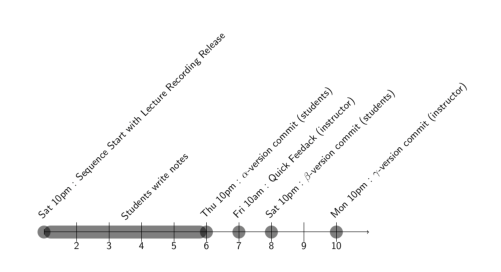
\includegraphics[scale=1.5]{scribe-timeline.pdf}
\end{center}

Even after these edits, it is possible that there are still errors in the draft, which may not get noticed. If you find errors still, please report to the instructor.


\newpage
\listofscribe
\newpage
\tableofcontents
\newpage
\listoftodos
\pagenumbering{arabic}
\setcounter{page}{1}
%\setstretch{1.1}

\Lecture{Jayalal Sarma}{Sep 9, 2020}{01}{Pigeon Hole Principle and Basic Applications}{Jayalal Sarma}{$\gamma$}{JS}

We start course with the simplest but surprising powerful tool in combinatorial arugments which is the pigeon hole principle. Through this principle as an example, we will also quick review the methods of proof. 

\section{Quick Recap on Proof Techniques} 

A formal mathematical proof system in our context has axioms about various mathematical objects that we are using, like numbers, graphs which describes them through their properties. Then, there are rules of inferences such as modus ponens, modus tollens, resolution, syllogisms etc which helps us derive new statements from these axioms. 

The peculiarity of these rules of inferences are that they "conduct truth"  and forms building blocks for huge "truth conducting" structures called mathematical proofs. That is, if for any object\footnote{a little more formally, the assignment in the propositional logic, and model in general first oder logic}, the premises of the rules of inference are true, then the conclusion is also true for them.   Hence, suppose we derive a statement $\phi$ starting with the axioms, applying the rules of inferences in various combinations. Since the individual rules of inferences "conduct truth", the resulting structure also conducts truth and is called the mathematical proof of the statement $\phi$ from the axioms. Note that the truth of the statement $\phi$ for the object under consideration can be stated on relative to the truth of the axioms that we used. However, this is not a concern, since we are intending to use the mathematical proof systems to derive statements about objects which we know would satisfy the axioms (in fact, we wrote down axioms as properties of those objects.
\begin{curiosity}
It is an amusing question to ask, whether there are other objects, which we did not intend to, which also satisfies the axioms that we wrote, by accident. Say for example, we wrote the axioms for graphs, but "strings" also satisfies them. If so, the theorems that we prove for graphs using only those axioms will also be true for strings, automatically !!. Quite interestingly this is true for natural numbers. The mathematical theory of natural numbers is axiomatized by what are called the Peano's axioms. There are numbers that one can define which are different from natural numbers for which any theorem that we prove for natural numbers also are true (because they satisfy the Peano's axioms). Then one might ask, are we not trying to represent exactly natural numbers? So should we not augment Peano's axioms with more properties of natural numbers such that we remove such {\em unwanted} parallel models from satisfying the axioms we write. Even more interestingly, one can argue that this is not even possible. No matter, what extra formula we write the existence of such "parallel models" us inevitable. In fact, not just one "parallel model", there will be infintiely many of them. You should read about {\em L\"owenheim–Skolem theorem}.
\end{curiosity}

Writing down mathematical proofs explicitly by using rules of inference may seem to be a mechanical way of proving statements. While it avoids any chance of mistakes because of the mathematical precision and rigor it affects quick readability and communication of ideas. Hence, one would like to have more "human readable" ways of representing these proofs by writing some of the steps in English, while ensuring that we do not lose the mathematical rigor. This brings in some subjectivity about how "formal" a proof is - that is, how close is it to the formal mathematical framework of rules of inferences in terms of notations, presentation etc.  Sometimes, very rigorous proofs tend to hide the intuitive idea behind the proof which one tends to (and sometimes need to) describe separately for easy communication. The more formal your proof is, the less chances of you making a logical error in the proof. It is a good idea to start writing proofs with the mindset of "rigor extremist" and once you are comfortable and see through the mathematically rigorous steps of a statement, you can rely more in English sentences. This course particularly would do it in the latter way, but ensuring that mathematical rigor is kept in tact. The beauty of the combinatorial proofs lies in the elegance and the combinatorial insight and intuition. Balancing the intuition with rigor in presentations and descriptions lies in the art of presentations.

Suppose that we have to prove a statement $\gamma$ of the form $p \rightarrow q$.  We quickly recall the different ways of proof in the above described form. 

\begin{description}
\item{\bf Direct Proof:} Assume $p$ and then derive $q$ using the assumption and the axioms by applying the rules of inferences. The is considered as a proof of the statement $p \implies q$ since it can be associated with a valid argument form by itself.
\item{\bf Indirect Proof:} Assume $\lnot q$ and then derive $\lnot p$. Again, this is also considered as a proof of the statement $p \implies q$ since it can be associated with a valid argument form by itself. This is also called proof by {\em contrapositive}.
\item{\bf Proof by Contradiction:}
A proof by contradiction, assumes the negation of the statement to be proven (that is, $\lnot \gamma$) and then defined a statement $r$ (this forms a part of creativitiy of the proof), and then derives $r \land (\lnot r)$ from the assumption and axioms using the rules of inferences. By an associated valid argument form, this shows that $\gamma$ must be true, again, by associating the definition of a valid argument form.
\end{description}
In addition, while proving quantified statements, there are a few additional ideas that are used which we quickly review below:
\begin{description}
\item{\bf Proof by Exhaustive Cases:} Suppose we want to derive a statement $\Gamma$ of the form $\forall \alpha P(\alpha)$ where $\alpha$ comes from domain of discourse $\cal{D}$ (say, for example, $\alpha$ is a natural number, that is, $\cal{D} = \N)$.  We can partition $\calD = \calD _1 \cup \calD_2 \ldots \cup \calD_k$ into several subdomains and prove the statement $\forall \alpha \in \calD_i,~P(\alpha)$ separately. Each part of the proof  $\forall \alpha \in \calD_i P(\alpha)$ is said to be a "case" of the proof. The fact that, $\calD = \calD_1 \cup \calD_1 \ldots \cup \calD_k$  is what is meant by the statement that the case analysis is {\em exhaustive}.
\item{\bf Proof by "Counter Example":} Suppose we want to disprove statements of the form $\forall \alpha P(\alpha)$. That is, we want to derive $\lnot\left(\forall \alpha P(\alpha)\right)$ which is logically equivalent to $\exists \alpha \lnot P(\alpha)$. Hence it suffices to demonstrate an $\alpha$ in the domain for which we can show $P(\alpha)$ is false.
\item{\bf Proof by Mathematical Induction:} This is a technique to prove statements of the form $\forall \alpha P(\alpha)$ where the domain $\calD$ is countably infinite. That is, the domain $\calD$ can be put in bijection with the set of natural numbers. The technique forms part of the Peano's axioms that define the natural numbers and hence is a valid proof technique. If $\phi : \N \to \calD$ is a bijection, in order to prove $\forall \alpha P(\alpha)$, we can equivalently prove $\forall n \in \N, P(\phi(n))$. In particular, it takes the following form:
\textit{If we can prove $P(\phi(0))$ and the implication $\left[ \forall  n \in \mathbb{N}, P(\phi(n)) \implies P(\phi(n+1) \right]$  then we can conclude  $\forall n~ P(\phi(n)) $}.
There are versions of this proof techniques such as strong induction, structural induction, spiral induction, double induction etc which are adaptations of the above basic idea.
\end{description}

Most of the proofs that we do in the courses will follow one of the above frameworks. We will not do examples of these techniques since that is already covered in the basic discrete mathematics course. 

\section{The Pigeon Hole Principle (PHP)}

With the quick recap done in the previous part, we now plunge into the actual business in this lecture. We first prove the following basic version of the Pigeon hole principle.
\begin{theorem}
Let $n,k \in \N$, such that $n > k$. Suppose we place $n$ identical balls in $k$ identical bins, then there is a bin that has  at least  two balls in it.
\end{theorem}
\begin{proof}
Let $n, k \in \N$ and $n > k$. Assume for the sake of contradiction that when we placed the balls into the bins as indicated in the theorem, there was no bin with at least two balls in it. 

As such the bins are identical, but number them from $1$ to $k$ now. Using this notation, let us define $b_i$ to be the number of balls that went into the bin number $i$. Clearly $\forall i, b_i \ge 0$. Since we did distribute all the balls into the bins, we have :
$$\calR : \sum_{i=1}^k b_i = n $$
Using the assumption, we have that: $\forall i, 0 \le b_i \le 1$. Summing up for $i$:
$\sum_{i=1}^k b_i \le \sum_{i=1}^k 1 = k < n$. Hence we have derived the statement :
$$\lnot \calR : \sum_{i=1}^k b_i \ne n$$
Hence we have derived $\calR \land \lnot \calR$. This is a contradiction and hence the original assumption that we started out with must be false and hence there has to exist a bin which has two balls in it.
\end{proof}

\begin{curiosity}
The formal proof of PHP as simple as it sounds is still a subject of substantial research in an area called \textit{proof complexity}. To demonstrate this, let us write the principle itself in more rigorous notations. Let $n > k$, and $\{ x_{ij} \mid  i \in [n], j \in [k] \}$ be propositional variables (which can be called, say {\em pigeon hole variables}). Following our original notation, where there are $n$ pigeons and $k$ holes, the basic Pigeon Hole Principle is the following Disjunctive normal form formula : 
$$\textrm{\sc PHP}_k^n \defn \left( \bigvee_{i \in [n]} \bigwedge_{j \in [k]} \bar{x_{ij}} \right) \lor \left( \bigvee_{j \in [k]} \bigvee_{r \ne s \in [n]} (x_{rj} \land x_{sj}) \right) $$
To prove this, one possibility is to derive the contradiction from the negation of 
$\textrm{\sc PHP}_k^n$. This is an expression in conjunctive normal form, with clauses:
$$ \textrm{For $i \in [n]$ the clauses : } Q_i \defn \bigvee_{j=1}^k x_{ij} $$
$$\textrm{ and for $s \ne t \in [n], j \in [k]$ the clauses } Q_{s,t,j} \defn \bar{x_{sj}} \lor \bar{x_{tj}}$$
Intuitively,  these say that there is a function from $[n] \to [k]$ (which is represented by $x_{ij}=1$ to mean that the function takes $i$ to $j$) which is well defined (for every $i$, there exists a $j$ such that $x_{ij} = 1$) and also injective (for two different $s$ and $t$, it is not the case that $x_{si}$ is $1$ and $x_{tj}$).
Since $n > k$, there cannot be an injection, and hence the negation of the conjunction of these clauses $\textrm{\sc PHP}_k^n$ must be true.

Suppose we ask, starting from these clauses as axioms, and applying rules of inferences (say the resolution principle) alone, how many steps of proof does one need to do to derive the contradiction ($r \land \lnot r$ for some $r$). \footnote{Notice that this sounds exactly like computation, how many steps of computation is required in order to certain tasks in terms of input parameters}. We measure this in terms of $n$ and $k$ which determines the number of variables in the system. The area which studies the complexity of proofs in the above is called {\em proof complexity theory}. It turns out the the basic PHP itself is one of the tautologies for which one requires exponentially long proofs if we are restricting ourselves to resolution? What if we relax this? The area has several interesting open questions related to this and they have close connections to computational complexity theory too.
\end{curiosity}

\subsection{A Quick Example: }

We will now demonstrate the application of the principle itself by a quick example. This is meant to be a revision of the topic from the previous courses and hence it is very much possible that you have seen the application earlier.

\begin{theorem}
If you consider any five points placed inside the unit square then there must necessarily exist two points are at most $0.75$ unit away from each other.
\end{theorem}
\begin{proof}
Firstly, to make it sound less magical, let us comment that  theorem is actually true for $0.75$ units replaced by $0.707$ units which is actually $\frac{1}{\sqrt{2}}$. The application of PHP goes as follows. Consider four small squares which are obtained by the midpoint of the square as one of the corners. These small squares form the bins and the five points that we place forms the balls. By applying PHP, we conclude that there must be two points which falls into the same small square. Now the argument can be completed by the fact that the maximum distance between any two points which are in the same small square is at most $\frac{1}{\sqrt{2}}$ since the sides of the square are $\frac{1}{2}$ each.
\end{proof}
\begin{remark}[{\bf Tightness}]
Is the above theorem tight? Can it be improved? Improvement can be in terms of two parameters. Firstly, can we make the same claim for 4 points? Secondly, even for 5 points, can we make an improved claim about the minimum distance being, say 0.7 units? The answer to both these questions are no. For the first, we can demonstrate  4 points in which every pair is at least one distance away - the four corners themselves will serve as a counter example. For the second question, we can demonstrate 5 points which are actually only pairwise at least $\frac{1}{\sqrt{2}}$ distance away. 
\end{remark}

\begin{remark}[{\bf Glimpse of Extremals in Combinatorics}]
The above example theorem, while is a classical application of Pigeon Hole Principle, it also demonstrates a curious phenomenon. In spirit it says that \textit{if there are large number of objects in a collection, then there must be some structure}. Question is how large? And what is structure? The answers to these vary and forms the foundations of this area. We will see more of this when we see Ramsey Theory.
\end{remark}

\section{Numbers and Remainders}

It is customary to do an example of PHP from numbers and division under remainders. We will do a slightly unusual example. 

\begin{theorem}
Consider the infinite sequence $7, 77, 777, \ldots ,7777777, \ldots $ - there must necessarily exist a number in this sequence that is divisible by 2003.
\end{theorem}
\begin{proof}
As weird as it sounds, one might wonder how does PHP play a role. There does not seem to be any place to apply PHP directly in the statement of the problem. Indeed, infinitude seems to indicate that we are allowed to take large numbers in the sequence. A usual trick is the division, and then consider the remainders.

As a start, consider  first 2003 numbers in the sequence. Denote them by $n_1, n_2, \ldots n_{2003}$. Divide them by 2003 and collect the remainders that we see. Denote them by $a_1, a_2, \ldots, a_{2003}$. If any of the $a_i$s are 0, then we are done since that  Indeed, we have that $1 \le a_i \le 2002$. Clearly, now the pigeons and holes are visible now. The numbers $n_i$s are the pigeons and the reminders are the holes. There are only 2002 holes but there are 2003 pigeons and hence by PHP, there must exists $1 \le i < j \le 2003$ such that $a_i = a_j$. This gives:
\begin{eqnarray}
n_i  \mod 2003 = n_j \mod 2003 \\
(n_i - n_j) \mod 2003 =  0\\
2003 \textrm{ divides } (n_i - n_j) \\
\end{eqnarray}

That is good progress. We managed to show 2003 divides $(n_i - n_j)$. However, $n_i - n_j$ unfortunately, will not be in the sequence at all. How will this number look like? By the structure of the numbers, subtracted, this difference will be a number of $7$s and then several zeros. More precisely computing these number, we have that:
$$(n_i - n_j) = n_{j-i} 10^{j-i}$$
So we have that $2003$ divides the product of $n_{j-1}$ and $10^{j-i}$. However, 2003 being an odd number which is not a multiple of $5$ will not have a common factor with any power of 10. Hence 2003 must necessarily divide $n_{j-i}$ which should be there in the sequence. This completes the proof.
\end{proof}

\section{Graphs}

Our third application is related to problems that can be modelled as graphs.

\begin{theorem}
In any chess tournament, where there are $n$ participants, at any point of time there must be two participants who finished the same number of games in the tournament.
\end{theorem}
It is natural to model this situation as a graph with $n$ vertices where each vertex represents a participant and we put an edge between two vertices if player $i$  and player $j$ have played a game with each other. The number of games played by a player is exactly the degree of the vertex in this graph. Rewriting the above theorem in the new language now:
\begin{theorem}
In any undirected graph $G$, there must be two vertices which are having the same degree.
\end{theorem}
\begin{proof}
The proof is by an exhaustive case analysis. We need to argue the above for all graphs. We divide this domain into two based on whether there is an isolated vertex or not.
\begin{description}
\item{\bf Case 1 : $G$ has an isolated vertex} - In this case, there is a vertex of degree $0$, and hence there cannot be a vertex of degree $n-1$. Thus we have $n$ vertices, and only $n-1$ possible degree values $\{10,,2,\ldots n-2\}$. By the PHP, we must see two vertices which has the same degree.
\item{\bf Case 2: $G$ does not have an isolated vertex} - In this case, there is no vertex of degree $0$, and hence the degree values of vertices can only be in the set $\{1, 2, \ldots n-1\}$. Again we have $n$ vertices whose degrees take only $n-1$ possible values. Again, by PHP, we must see two vertices having the same degree.
\end{description}
\end{proof}

\begin{exercise-prob}[See Problem Set 1~(Problem \ref{mutual-friends})]
\begin{show-ps1}{mutual-friends}
A social network is said to be symmetric if the relation between users that is maintained as a part of the network, is symmetric. Consider a symmetric social network  and let the symmetric relation maintained be that of ``user $A$ and $B$ are {\em friends}" (like in the case of facebook). A user $C$ is said to be a \textit{mutual friend} of users $A$ and $B$ if, $C$ is a friend of both $A$ and $B$. Prove that - for any user $A$ of the network who has at least two friends, there must exist two friends of $A$ who has the same number of mutual friends with $A$. 

Comment on whether symmetry is critical for your argument. Take the example of {\em instagram} where the symmetric relation of {\em friends} is replaced by {\em followers}. Generalize the definition of mutual friends to {\em mutual followers}. Comment on whether a similar statement for followers can be established in this case.
\end{show-ps1}
\end{exercise-prob}

\section{Discussion Session}

Just to get started, we considered the following question - \textit{how many people do we need to choose so that we can be assured that two among the set of people we have chosen will have their birthday on the same day?} The answer to this question is given by Pigeon Hole Principle immediately by considering the people to be pigeons and the day of the year on which their birthday falls to be the pigeonhole. Hence to be guaranteed that out of the 366 holes, at least one contains two pigeons (people), and hence having the same birthday, we need to choose 367 people. Just to test our understanding, we asked "is the theorem tight?" in terms of number of people. It is indeed is, since there is a set of 366 people whom you can choose all of whom have different birthdays. That is, 367, is the smallest number for which the above statement can be proposed. Hence the theorem is tight.

The first discussion point that was raised was a comparison with Birthday paradox. If we do not choose 367 people we are not given the guarantee that there are two people in the set with same birthday. What if we don't want this guarantee with certainty - but instead, we will need to get a probabilistic guarantee. To formalize this one has to imagine an experiment where the people are chosen uniformly at random. More rigorously, the property of the distribution is that for every date of the year, the probability that the chosen person has a birthday on that day is $\frac{1}{365}$. Let us say, we are talking about a non-leap-year. The questions is then of the form {\em what is the minimum number of people we need to choose, as per the above experiment, such that we are guaranteed at least 99.999\% chance of getting two people with the same birthday in the set?}. A natural number to choose is 364 which is slightly less than 365. But what is the minimum? The answer beats our usual intuition and is surprisingly low - we need to choose only 70 people to achieve this !!. The surprise goes even further if we ask for 50\% success, then the number is just 23 !! - and hence this is called \textit{the birthday paradox}.

\subsection{Impossibility of Perfect Lossless Compression}

PHP has a variety of applications. A first application outside discrete math course, that we usually encounter is in the automata theory where we use it to prove the pumping lemma. In fact, this one principle is pivotal in showing that there {\em cannot be} finite automaton accepting certain languages.

We then turned into a practically related application of PHP, in the context of file compression. We all have used file compression programs - say like zip or tar. They compress our files into smaller sizes and they usually provide compression ratio too. Here is a question out of curiosity. Can we give compression algorithm that is guaranteed provide compression for all the files? This is a natural requirement. Interestingly, the actual situation is worse, any compression algorithm, not only cannot reduce the size of all files, but also has to increase the size of some file. The argument uses PHP. 

Compression algorithms are nothing but programs which translates files (which are interpreted as strings) to strings. That is, they are functions of the form $C : \Sigma^* \to \Sigma^*$. A compression algorithm is said to {\em lossless} if this function is injective. That is, given a compressed strings (element in the RHS) we have a unique file that we can decompress it to. Indeed, compression algorithms that are not lossless are practically useless since there cannot exist decompression algorithms which can recover the compressed file.

\begin{theorem}
For any lossless data compression algorithm that makes at least one file smaller, there will be at least one file that it makes larger.
\end{theorem}
\begin{proof}
Let $C$ be the compression function from $\Sigma^* \to \Sigma^*$. Let us fix $\Sigma = \{0,1\}$ without loss of generality.
Suppose it makes at least one file smaller than its size as a result of the compression. In addition, for the sake of contradiction, suppose that the algorithm does not make any file larger than their respective sizes.  Let $w \in \Sigma^*$ be the shortest string (say, $|w| = \ell$) which the algorithm makes smaller. That is, by the assumption, for $w' \in \Sigma^*$ such that $|w'| < |w|$, $|C(w')| = |w'|$. Thus, consider the following set :
$$ \Gamma = \left\{ w \in \Sigma^* \mid | C(w) |  < \ell \right\} $$
From the above assumptions, we have that $|\Gamma| \ge 2^\ell+1$, but then by definition $\Gamma \subseteq \{0,1\}^{\ell-1}$. Hence by Pigeon Hole Principle, $\exists w,w' \in Gamma$ with $w \ne w'$, such that $C(w) = C(w')$. This contradicts the lossless property.
\end{proof}
%
%\subsection*{Computation of $M$ - from discussion on Sep 28th}
%
%\paragraph{Harmonic Number Bound:}
%
%\begin{eqnarray*}
%H_n & = & 1+\frac{1}{2}+\frac{1}{3}+\frac{1}{4} \ldots +\frac{1}{n} \\
%& = & \bigsum_{k=0}^{\lfloor \log n \rfloor} \sum_{j=0}^{2^k -1} \left( \frac{1}{2^k+j} \right) \\
%& \le & \bigsum_{k=0}^{\lfloor \log n \rfloor} \sum_{j=0}^{2^k -1} \left( \frac{1}{2^k} \right) \textrm{ since the denominator decreased} \\
%& = &  \sum_{k=0}^{\lfloor \log n \rfloor} (1) \le \log n 
%\end{eqnarray*}
%We wanted to compute :
%
%\[ M = \sum_{d=1}^\infty \frac{\mu(d)}{d^2} \]
%
%By using prime decomposition theorem, if $p_1,p_2, \ldots $ are list of primes:
%
%\[ M = \left( 1- \frac{1}{p_1^2} \right) \left( 1- \frac{1}{p_2^2} \right)  \left( 1- \frac{1}{p_3^2} \right)  \ldots \]
%
%The next idea is to compute $\frac{1}{M}$ as follows: since we have written above as the product -
%
%\begin{eqnarray*}
%\frac{1}{M} & = & \frac{1}{\left( 1- \frac{1}{p_1^2} \right) }  \frac{1}{\left( 1- \frac{1}{p_2^2} \right) }  \frac{1}{\left( 1- \frac{1}{p_3^2} \right) } \ldots \\
%\end{eqnarray*}
%Using the infinite series expansion ... $\left(1-\frac{1}{x^2}\right() = 1+x^2+x^4+\ldots$
%\begin{eqnarray*}
%\frac{1}{M} & = & \left( 1+\frac{1}{p_1^2} + \frac{1}{p_1^4} \ldots \right)
%\left( 1+\frac{1}{p_2^2} + \frac{1}{p_2^4} \ldots \right)
%\left( 1+\frac{1}{p_3^2} + \frac{1}{p_3^4} \ldots \right) \\
%& = & 1+\frac{1}{2^2}+\frac{1}{3^2}+ \ldots \\
%& = & \frac{\pi^2}{6} \textrm{   {\tt By Euler sum that Gautam mentioned in the session}}
%\end{eqnarray*}


\Lecture{Jayalal Sarma}{Sep 9, 2020}{02}{More on PHP}{Jayalal Sarma}{$\gamma$}{JS}

\section{Warm up and  Generlizations of PHP}

We start with a usual application of PHP to numbers to warm up in the lecture.
\begin{theorem}
In any set of $n+1$ positive integers each at most $2n$, there must exist at least one number which divides the other. 
\end{theorem}
\begin{proof}
Let $S = \{a_1, a_2, \ldots , a_{n+1}\}$ be the set of $n+1$ positive integers such that $a_i \le 2n$. Each number can be written in the form $a_i = 2^{k_i}q_i$ where $k_i$ is the maximum power of $2$ that divides $a_i$ and $q_i$ hence is an odd number.

Now consider the numbers $q_1, q_2, \ldots q_{n+1}$. Can they be distinct? Since they all are in the range $1 \le q_i \le 2n$, where there are only $n$ odd numbers - By an application of PHP, we have that there must exist $i, j$ such that $1 \le i \ne j \le n+1$ with $q_i = q_j$.  Hence, we have that $k_i \ne k_j$. This gives the two exhaustive cases:

\begin{description}
\item{{\bf Case 1:} $k_i > k_j$:} Since $2^{k_j}$ divides $2^{k_i}$ and this gives $q_j2^{k_j}$ divides $q_i2^{k_i}$. Hence $a_j$ divides $a_i$.
\item{{\bf Case 2:} $k_j > k_i$:} Same as previous case, just swapping the role of $i$ and $j$.
\end{description}
In either case, we have that there exists two numbers in the set where one divides the other. This concludes the proof.
\end{proof}

We now state a usual generalization of PHP as a recap.

\begin{theorem}[{\bf Generalized of PHP}]
Let $n,m ,r$ be positive integers and let $n > mr$. If we distribute $n$ balls into $m$ bins, then there must be a bin which has at least $r+1$ balls.
\end{theorem}

Indeed, the generalization comes handy when the combinatorial statement that we want to explore is not about a "conflict" but about multiple elements getting to same bag. A simple recap example to demonstrate this is the following question - {\em how many students do we need to be in the course, such at the end of the semester, no matter how the performance of the students is, that at least five students get the same letter grade (out of the five grades $S,A,B,C,D,E$)?} This is also an extremal question. Applying generalized PHP, with $r+1 = 5$ and $m=6$, it is sufficient to have 25 students in the class.  And with 24 we cannot guarantee this since there is way to distributed 4 students each to each grade so that there are not 5 students having each grade.

\section{Example 2 : Erd\"os-Szekeres Theorem}

This is about a pattern that appears in sequence of distinct numbers first proved by Erd\"os and Szekeres in 1939. The theorem its has a geometric interpretation too. The theorem itself is a creative use of Pigeon Hole Principle and is a case of extremal combinatorics.

\begin{theorem}
In any Sequence of $n^2+1$ distinct real numbers there must necessarily exist either a strictly increasing subsequence  of $n+1$ numbers  or a strict decreasing subsequence of $n+1$ numbers.
\end{theorem}
Before we begin to prove this, let us play around with an example.
$8, 11, 9, 1, 4, 6, 12, 10, 5, 7$. Here $n=3$ and there are 10 numbers in the sequence. There must be at least one strictly increasing subsequence of length 4. Indeed, there is - the subsequence $1,4,6,12$. In fact, there are more, $1,4,6,10$ etc. But anyways there is at least one. In fact, in this case, it so happens that there is a strictly decreasing sequence also of length $4$. This is the subsequence, $11, 9, 6, 5$. There are more subsequences.

\begin{proof}
The proof is an elegant and intuitive one. A perfect example of how such proofs are discovered. Suppose $a_1, a_2, \ldots a_{n^2+1}$ forms the given sequence of numbers.

Suppose we checked for the increasing subsequence of numbers of length $n+1$ and for decreasing subsequence of length $n+1$ but did not find it in the above sequence. How do we formally represent this data? Here is an idea, for each index $k$, let us associate a pair of numbers $(i_k,d_k)$, which are defined as : the length of longest increasing (for $i_k$ and respectively decreasing for $d_k$) subsequence of numbers starting from the number $a_k$ in the given sequence. The reason we failed to find the subsequence indicates that these pairs must satisfy, for every $k$, $1 \le i_k \le n$ and $1 \le d_k \le n$.

Thus we have $n^2+1$ tuples in hand where value for each component can be only between $1$ and $n$. Hence there are only $n^2$ different distinct such pairs possible. But now we have a scenario for PHP, which gives that there must exist $s,t \in [n^2+1]$ such that $s \ne t$ (say without loss of generality that $s > t$) such that the tuples for both these indices are the same. That is $i_s = i_t = i$ (say) and $d_s = d_t = d$ (say).

We know that the numbers are distinct in the sequence. Hence $a_s \ne a_t$. Thus we have the following two exhaustive cases:

\begin{description}
\item{{\sf Case 1:} $a_s > a_t$ :} Let $(t_1, t_2, \ldots t_d)$ be the decreasing sequence of length $i$ that starts from $a_t$ with $t_1 = a_t$. But then $(a_s, t_1, t_2, \ldots t_d)$ is also decreasing and it starts with $a_s$ and is of length $i+1$. This contradicts the fact that $d_s = d$.
\item{{\sf Case 2:} $a_s < a_t$ :} Same as the above case, where we replace decreasing with increasing and the final contradiction is for the fact that $i_s=i$, because we can demonstrate a length $i+1$ increasing subsequence of length $i+1$ in the given sequence.
\end{description}
Hence the proof.
\end{proof}

\begin{remark}
The above theorem can also be generalized, and in fact is the original form of the Erd\"os-Szekeres theorem. For given natural numbers $r$, $s$ they showed that any sequence of distinct real numbers with length at least $(r-1)(s-1)+1$ contains a monotonically increasing subsequence of length $r$ or a monotonically decreasing subsequence of length $s$. 
\end{remark}

\section{Example 3: People at Party}

If $6$ people are invited to a party, something interesting happens. Let us say some pairs of them are friends and some pairs of them are strangers with each other. There will always be some set of three people who are pairwise strangers with each other or there will be a set of three people who are pairwise friends with each other. This phenomenon can be easily mistaken to be a sociological or behavioural psychological fact that humans seem to be behave this way. However, it turns out that it can be seen as a simple result of combinatorics and is a nice applciation of PHP in disguise. We demonstrate this now.

\begin{theorem}
If $6$ people are invited to a party, then there must exist three of them who are pairwise strangers each other, and there must be three of them who are pairwise  friends with each other. 
\end{theorem}
There are many equivalent ways of formulating this. One can talk about graphs to model the facts stated above. We defer these to a later point when we get to Ramsey numbers. We now get to the proof of the above in the same language as we discussed above.
\begin{proof}
Let $P$ be the set of people who joined the party. Let $\alpha \in P$ be one of the attendees. We do the following case analysis based on how many people does $\alpha$ are friends with in the party. We want to demonstrate a set $\Gamma \subseteq P$ such that $|\Gamma| = 3$ and the members of $\Gamma$ are either pairwise friends or pairwise strangers.
\begin{description}
\item{{\bf Case 1:} $\alpha$ has atleast three friends in $P$:} Let $\beta, \gamma, \delta$ be the three friends. We ask the question, are $\beta, \gamma, \delta$ friends amongst themselves? The answer to this will give the following exhaustive subcases.
\begin{description}
\item{{\bf Case 1a:} $\beta, \gamma, \delta$ are pairwise strangers among each other:} In this case  we can simply set $\Gamma = \{ \beta, \gamma, \delta \}$ which has the required property for $\Gamma$ as desired.
\item{{\bf Case 1b:} there is a pair among $\beta, \gamma,$ and $\delta$ who are friends :} Without loss of generality let us say $\beta$ and $\gamma$ are friends (the other cases are similar). In this case, define $\Gamma = \{\alpha, \beta,\gamma\}$ and it has the desired properties.
\end{description}
\item{{\bf Case 2:} $\alpha$ has at most two friends in $P$}. In this case, there are three strangers for $\alpha$ in $P$, and let us name them $\beta, \gamma, and \delta$. We ask the question, are $\beta, \gamma, \delta$ friends amongst themselves? The answer to this will give the following exhaustive subcases.
\begin{description}
\item{{\bf Case 2a:} $\beta, \gamma, \delta$ are pairwise friends among each other:} In this case  we can simply set $\Gamma = \{ \beta, \gamma, \delta \}$ which has the required property for $\Gamma$ as desired.
\item{{\bf Case 2b:} there is a pair among $\beta, \gamma,$ and $\delta$ who are strangers :} Without loss of generality let us say $\beta$ and $\gamma$ are the strangers (the other cases are similar). In this case, define $\Gamma = \{\alpha, \beta,\gamma\}$ and it has the desired properties.
\end{description}
\end{description}
Since we argued in both the cases, this completes the proof of the theorem.
\end{proof}
\begin{remark}
A more elegant way to handle case 2 is to reduce it to case 1 itself. Consider the complement of the friends/stranger relation. Note that the result required for the theorem does not change since we just need $\Gamma$ to be either pairwise strangers or pairwise friends and they just get complemented. Now, if $\alpha$ has at most two friends in $P$, it has at least three friends in $P$ in the complementary relation and hence we can reuse Case 1 in this case.
\end{remark}

\begin{exercise}
Is the above theorem tight? Indeed, one can construct 5 people going to a party and associate a friends/stranger relation among them such that there does not exist three people who are friends with each other and  there does not exist three people who are strangers with each other. The exercise is to explicitly write down this counter example relation.
\end{exercise}

\begin{exercise-prob}[See Problem Set 1~(Problem \ref{php-square})]
\begin{show-ps1}{php-square}
The set $M$ consists of nine positive integers, none of which has a
prime divisor larger than six. Prove that $M$ has two elements whose
product is the square of an integer. Is the bound $9$ in the above statement tight?
\end{show-ps1}
\end{exercise-prob}

\Lecture{Jayalal Sarma}{Sep 10, 2020}{03}{PHP for Dirichlet's Approximation Principle}{Jayalal Sarma}{$\gamma$}{JS}

We now discuss a very old and different application of PHP which predates the name PHP itself. This is to show the approximation principle of irrational numbers. This application got this principle the name as {\em Dirichlet Box Principle}.

\section{Approximation of irrationals by rationals}
The task we have at hand is about approximating irrational numbers using rationals to a given accuracy. As a concrete example, suppose we want to approximate $\sqrt{2}$ by $\frac{p}{q}$ up to a given accuracy $\epsilon$ such that
$$ \left| \sqrt{2} - \frac{p}{q} \right| \le \epsilon $$
the driving question for us, is how large should $p$ and $q$ be? In fact they are related and hence, we need to ask how large the denominator $q$ should be? The larger the $q$ is, the more the granularity of the representation is, and the larger the storage cost is for the number to be represented. Hence, for a fixed irrational number and a given $\epsilon$ we want the value of $q$ to be as small as possible.

Indeed, if we want to do this for an arbitrary irrational number, here is a simple idea: let $q \in \N$ (which we will choose later). Divide the number line into intervals of length $\frac{1}{q}$ each. Consider the number $\alpha$ and see which interval it belongs to. Choose the nearest multiple of $q$ to be the $\frac{p}{q}$ to be the approximation of $\alpha$. A quick thought will convince you that the error introduced by this method is at most half of the interval size which is $\frac{1}{2q}$. That is, for any $q$ that we choose, if we choose $p$ also accordingly as above,
$$ \left| \alpha - \frac{p}{q} \right| \le \frac{1}{2q} $$
Thus, for a given $\epsilon$, we should choose $\frac{1}{2q} < \epsilon$ to get the required accuracy. In other words, $q$ linearly changes with $\frac{1}{\epsilon}$. Just to get a sense of this growth, if $\epsilon$ is given to be $0.0001$, then we should choose $q$ to be roughly 5000. 

\section{Dirichlet's Approximation Principle}

Indeed, we would have probably preferred a smaller $q$, due to the above mentioned representation cost. Dirichlet approximation principle, exactly improves the above and is a nice application of the pigeon hole principle.

\begin{theorem}[{\bf Dirichlet's Approximation Principle}]
For every irrational number $\alpha$, there is a $p, q \in \Z$ such that:
$$\left| \alpha - \frac{p}{q} \right| < \frac{1}{q^2}$$
\end{theorem}

A few remarks about the improvement  is due. Indeed, now $q$ changes quadratically with $\epsilon$. To check the numbers, suppose $\epsilon$ is given to e $0.0001$, then we can afford to choose $q$ to be just 100, as opposed to 5000.  We will now prove the above theorem:

\begin{proof}
Let $\alpha$ be the irrational number that we are interested in approximating.
First observation is that it is sufficient to prove that $\exists p,q \in \Z$,
$$\left| q\alpha - p \right| < \frac{1}{q}$$
In other words, we need to understand the nearest integer to the quantity $q\alpha$. Intuitively, the fractional part of $q \alpha$ plays a roles in this and which we will study now.

Fix a positive integer $N$ (we will choose this later) and consider the numbers $0, \alpha, 2\alpha, \ldots N\alpha$. Ideally we will choose $q$ to be less than $N$, hence one of these numbers is $q \alpha$. However, since we are interested in the fractional parts, let us distribute them into intervals as we did in the naive case.

Consider the interval from $[0,1)$ divided into subintervals of the form:
$$ \left[\left.0,\frac{1}{N}\right.\right),\left[\left.\frac{1}{N},\frac{2}{N}\right.\right) \ldots ,\left[\left.\frac{N-1}{N},1\right.\right) $$

There are $N$ intervals in this list. If we distribute the fractional part of $N+1$ numbers $0, \alpha, 2\alpha, \ldots N\alpha$ to this list, by PHP, we have that there must be two of the multiples of $\alpha$ which falls within the same interval. In other words, there exists $a,b \in \{0,1, \ldots N\}$ such that:
$$ \{a\alpha\} - \{b \alpha\} < \frac{1}{N}$$
Just to fast forward, the idea is to demonstrate that the choice of $q = a-b$ actually works for our purpose. To do this, we will show that the nearest integer to $a \alpha  - b \alpha$ is at most $\frac{1}{a-b}$ away from it and that integer will be our $p$. Since $a-b$ is at most $N$, it is sufficient to show that there is an integer close to $a \alpha  - b \alpha$ is at most $\{a \alpha \} - \{b \alpha\}$ away. By the above, we have that this is at most $\frac{1}{N}$ which in turn is at most $\frac{1}{a-b}$. This is in fact a general statement which we can prove as follows:

\begin{lemma}
\label{lem:a-b}
Let $A$ and $B$ be two real numbers, there is  an integer $p$ close to $|A-B|$ such that:
$$d(p,|A-B|) \le \{A\} - \{B\} $$
where $d(s,t)$ denotes $|s-t|$.
\end{lemma}
\begin{proof}
The idea is very simple, let us write:
$A = A_1+A_2 \textrm{  and } B = B_1+B_2$
where $A_1$ and $A_2$ are integral and fractional part respectively. If $A_2 > B_2$, then the distance to the integer $|A_1 -B_1|$ is at most $A_2-B_2$. The other case works in a similar way.
\end{proof}

Applying Lemma~\ref{lem:a-b} to the case when $A = a\alpha$ and $B = b \alpha$, gives us that there is an integer $p$ such that 
$$d(p,|a\alpha - b\alpha|) \le |\{a\alpha\} - \{b\alpha\}| < \frac{1}{N} \le \frac{1}{a-b} = \frac{1}{q}$$
Thus, there is $p$ (as claimed by Lemma~\ref{lem:a-b}) and $q$ (which is equal to $a-b$ which exists as per PHP application), such that:
$$|q\alpha - p| \le \frac{1}{q}$$
This completes the proof of the theorem.
\end{proof}


\begin{exercise-prob}[See Problem Set 1~(Problem \ref{simultaneous-approx})]
\begin{show-ps1}{simultaneous-approx}
Let $\alpha_1, \alpha_2, \ldots \alpha_k$ be $k$ rational numbers. Generalizing the Dirichlet's approximation principle argument that we did in class, using PHP again, prove that there must exist integers $p_1, p_2, \ldots p_k$ and $q$ such that:
$$\forall i,~\left| \alpha_i - \frac{p_i}{q} \right| < \frac{1}{q^{1+\frac{1}{k}}}$$
\end{show-ps1}
\end{exercise-prob}

\begin{remark}
The proof of the theorem proves something stronger. That is, it actually can give a way to get many $q$'s which acheive the error bound. Notice that the choice of $N$ was free in the proof and $q$ that we end up choosing is $a-b$ which is at most $N$. Hence suppose that we already have a $p$ and $q$ in hand, if we run the proof by choosing $N$ to be large enough such that:
$$\frac{1}{N} < |q\alpha - p|$$
then necessrily the new $p$ and $q$ that the proof gives will have to be different (and $q$ needs to be larger). By repeating this, we can produce a new $p$ and $q$ and so on and so forth. This gives us a way to produce infinitely many $p$ and $q$ such that:
$$\left| \alpha - \frac{p}{q} \right| < \frac{1}{q^2} $$
\end{remark}

We were clearly motivated to improve the denominator of $2q$ in the naive attempt to $q^2$ in the denominator in the rational approximation principle. Can this be improved further? The following curiosity remark says otherwise.

\begin{curiosity}[{\bf Tightness of Dirichlet's Approximation Principle - Roth's Theorem}]
Let $\alpha$ be any algebraic number (which can be expressed as the root of a polynomial with coefficients from $\mathbb{Q}$. For every $\epsilon$ the inequality,
$$\left| \alpha - \frac{p}{q} \right| < \frac{1}{q^{2+\epsilon}}$$
can hold true only for finitely many co-prime pairs $(p,q)$. This says that the Dirichlet's approximation principle cannot be improved (for infinitely many $p$ and $q$) with a larger order denominator.
\end{curiosity}

The above remark says that we cannot improve in the exponent for Dirichlet's approximation principle. Can we improve by having a large multiplier for the $q^2$ in the denominator? Even this has a limit, and leads to classifying irrational numbers using what is called the \textit{Lagrange measure} of the number.

\begin{curiosity}[{\bf Hurwitz Theorem and Irrationality Measures}]
This is an improvement of the above principle. For every irrational number $\alpha$, there are infinitely many relatively prime integers $p$ and $q$ such that:
$$\left| \alpha - \frac{p}{q} \right| \le \frac{1}{\sqrt{5}q^2}$$
The $\sqrt{5}$ in the denominator is the best possible. If we let it greater than $\sqrt{5}$, then there is a counter example - consider the irrational number $\frac{1+\sqrt{5}}{2}$ (the golden ratio). It can be shown that this can have only finitely many relatively prime integers $p$ and $q$ with the above formula holding (this is done through arguments about continued fraction representations). For example, if we avoid \textit{golden ratio} and some similar irrational numbers, then we can improve the denominator to $\sqrt{8}$. If we avoid \textit{silver ratio} ($1+\sqrt{2}$) and associated irrational numbers, then we can improve this to $\frac{\sqrt{221}}{5}$. In general, the bound is of the form:
$$\left| \alpha - \frac{p}{q} \right| \le \frac{1}{L_nq^2}$$
where $L_n$ (called the \textit{Lagrange numbers}) steadily increases if some bad irrational numbers are included. These also are viewed as measures of "how much irrational the number is". 
\end{curiosity}

\Lecture{Jayalal Sarma}{Sept 14, 2020}{04}{Counting by Bijections and Double Counting Principle}{Jayalal Sarma}{$\gamma$}{JS}

We now quickly review the basic tools from counting. Permutations and combinations forms the basics from discrete mathematics that we rely upon. We will stress on the aspects that are critical for the rest of the course. The first tool that we will demonstrate in detail is the power of counting by using bijections.

\section{Basic Examples of Counting by Bijections}

The cardinality of two sets is said to be the same if there is a bijection between the two. Indeed, for finite sets the notion of cardinality matches with that of size while it can be deceiving for infinite sets\footnote{For infinte sets, there are notions of countability and uncountability of sets which we will not discuss here.}. We will concentrate on finite sets for this part and use bijections to establish combinatorial counting.

We start with something that we are all familiar with, in order to bring out the nuances involved with proof by bijections. Notice that we know how to count this object even otherwise, by other means, but this is just as a starting example.

\begin{proposition}
The number of subsets of a set is of $n$ elements is exactly $2^n$.
\end{proposition}
\begin{proof}
Let $S$ be the given set of $n$ elements. Without loss of generality let us assume that $S = \{1,2,\ldots, n\}$. The bijection is nothing but the well-known idea of characteristic vector of a set,

We establish a bijection between the following two sets.
$$ \phi : \left\{ A : \begin{array}{c} A \textrm{ is a subset of } \\ \textrm{ the set $S$ } \end{array} : \right\} \to \left\{ x : \begin{array}{c} x \textrm{ is a string of length $n$} \\ \textrm{ over alphabet $\{0,1\}$ } \end{array} : \right\}$$
We first define the function as follows. Let $A$ be any subset of $S$, define the string $w = \phi(x)$ as the $n$-bit string where for every $1 \le i \le n$:
\[
w_i = 
\begin{cases}
0 & \textrm{ if $i \notin A$ }\\
1 & \textrm{ if $i \in A$ }
\end{cases}
\]

Notice that the function $\phi$ is well-defined (this may have to be checked explicitly in certain bijections when we define) since we are defining the bit $w_i$ for every $i \in [n]$. 

We now argue that it is an injection. Suppose that two sets $A, B \subseteq S$, but $A \ne B$. That is there is an $i \in S$ for which $i \in A$, but $i \notin B$. By the above definition, the $i$-th but of $\phi(A)$ will be $1$ while the $i$-th bit of $\phi(B)$ will be $0$. This implies $\phi(A) \ne \phi(B)$.

We also show that $\phi$ is a surjection. Given any $w \in \{0,1\}^n$, we can define a pre-image $A \subseteq S$ as $A = \{ i \mid w_i = 1 \}$. By definition, $\phi(A) = w$ and hence $w$ has a pre-image. This shows $\phi$ is a surjection.

\end{proof}

Let us argue a slight variant of the above example now. While there are other ways to establish this, we insist on using the method of counting by bijections.

\begin{proposition}
The number of even sized subsets of $[n]$ is equal to the number of odd sized subsets, and both are equal to $2^{n-1}$.
\end{proposition}
\begin{proof}
by observing that the bijection that we defined in the previous proof has the additional feature that the number of $1$s in $\phi(A)$ is exactly the cardinality of $A$, we can conclude that it is sufficient to establish a bijection between the following two sets:
$$ \psi : \left\{ x : \begin{array}{c} x \in \{0,1\}^n \textrm{ having } \\ \textrm{even no. of 1s in it}  \end{array} \right\} \to \left\{ w : \begin{array}{c}  \textrm{ $w \in \{0,1\}^n$ having} \\ \textrm{odd no. of 1s in it}  \end{array} \right\}$$
Fix any $i \in [n]$, we define a bijection with respect $i$ (this says there are actually $n$ bijections between the two sets above, not just one !). Technically, we should be writing $\psi_i$ but we drop the subscript since it is not critical for the representation. 
\begin{description}
\item{\bf Definition:} We define the bijection as follows : let $e_i$ denote the string which has $1$ in the $i$-th position and $0$ elsewhere.
$$\psi(x) = x \oplus e_i $$
where $\oplus$ denotes bitwise xor to produce an $n$ bit string.
\item{\bf well-defined:} We explicitly check whether the function is well-defined. Indeed, consider any $x \in \{0,1\}^n$ which has even number of $1$s in it. By the operation $x \oplus e_i$ produces a string in $w \in \{0,1\}^n$. Since the $i$-th bit is flipped, $w$ must necessarily have odd number of 1s in it.
\item{\bf injection:} 
We show that $\psi$ is an injection. Consider $x, x' \in \{0,1\}^n$ such that $x \ne x'$.  There must exist an index $j$ in which they differ. We have two cases:
\begin{description}
\item{{\bf Case 1:} $j = i$ :} Indeed, since the $i$-th bit is flipped by the mapping, the images $w = \phi(x)$ and $w' = \phi(x')$ must also have their $j$-th bit to  be different. Hence $\phi(x) \ne \phi(x')$.
\item{{\bf Case 2:} $j \ne i$ :} Since the operation does not change any other bit. The images $w = \phi(x)$ and $w' = \phi(x')$ must also have their $j$-th bit to  be different. Hence $\phi(x) \ne \phi(x')$.
\end{description}
Hence, we conclude that $\phi$ is injective.
\item{\bf surjection:} Given any $w \in \{0,1\}^n$ which has odd weight, we show $x \in \{0,1\}^n$ such that $\phi(x) = w$. Indeed, defining $x = w \oplus e_i$ will meet the requirement. Hence $\phi$ is surjective.
\end{description}
Hence we conclude that $\phi$ is a bijection and that the two sets must be of same cardinality. Since the two sets are disjoint and their union is of size $2^n$, it must be that both of them are of size $2^{n-1}$. This concludes the proof.
\end{proof}

Note that in the above proof, we wrote down the steps in proving the bijection explicitly. It is somewhat standard to skip over the one which are obvious from the definitions, but it is a good practice to write these down in a formal proof so that the argument is not prone to errors.

\subsection{Discussion Session - Counting Cyclic Triplets}

We considered the following counting question in the discussion session to demonstrate that simple bijection and the idea of associating combinatorial objects is a very powerful combinatorial technique.

\begin{problem}
Imagine there are $2n+1$ players in a round-robin tournament. That is, each player plays against every other player. Assume that there are no ties in any match. We say that players $\{a,b,c\}$ forms a cyclic triplet if $a$ beats $b$, $b$ beats $c$, and $c$ beats $a$ (note that the order does not matter). We want to count the maximum number of cyclic triplets that is possible in the tournament.
\end{problem}
\begin{proof}
It is natural to model the above using graphs where each vertex is a player and two vertices $(i,j)$ is a directed edge if the player $i$ beats player $j$. This gives a directed graph with $2n+1$ vertices whose underlying undirected graph is a complete graph on $2n+1$ vertices. It is also called a tournament. Cyclic triplets can naturally be associated with triangles in these directed graphs. So the statement we are address is also equivalently stated as {\em in any tournament on $2n+1$ vertices, what is the number of triangles?}.

The idea is to look at associated objects called "corners" of the triangles. There are ${2n+1 \choose 3}$ triangles, and hence there are $3 {2n+1 \choose 3}$ many corners. The corners can be classified into three types.
\begin{description}
\item{\bf Type 1:} A corner where both edges are incoming edges.
\item{\bf Type 2:} A corner where both edges are outgoing edges.
\item{\bf Type 3:} A corner where one edge is incoming and the other is outgoing.
\end{description}

What happens in a cyclic triplet? It forms a triangle, hence the three corners has to be of Type 3. A non-cyclic triplet will have one corner of each Type. This also establishes a bijection between the Type 1 and Type 2 corners as follows.

$$ \psi : \left\{ \begin{array}{c} \textrm{Type 1} \\ \textrm{Corners}  \end{array} \right\} \to \left\{ \begin{array}{c} \textrm{Type 2} \\ \textrm{Corners}  \end{array} \right\} $$

defined as follows: given any corner $c$ of type 1, define $\psi(c)$ as the type 2 corner that appears in the (undirected) triangle that this corner appears in. This is well defined because (1) $c$ cannot appear in a triangle corresponding to the cyclic triplet (2) exactly only type $2$ triplet can appear in a triangle corresponding to non-cyclic triplet. This uniquely assigns a type 2 corner with $c$ and makes the function, well-defined, injective and surjective (since the process can be reversed too). In fact, the same bijection also proves that the number of non-cyclic triplets is exactly the number of Type 1 corners and also exactly equalt to the number of Type 2 corners. Hence it sufficient to count the number of Type 1 corners. 

So now the strategy is clearer. To obtain an upper bound on the number of cyclic triplets, we express it ${2n+1 \choose 3}$ minus the number of non-cyclic triplets. The it suffices to obtain a lower bound for the number of non-cyclic triplets. Hence it suffices to obtain a lower bound on the number of type 1 corners (or equivalently the number of type 2) corners.

One natural attempt is to aim to count type 1 corners alone. If $d_i$ is the in-degree of the $i$-th vertex, then the number of type 1 corners can be estimated as :

$$t_1 = \bigsum_{i=1}^{2n+1} {d_i \choose 3}$$

However, it is unclear how to get a reasonably tight lower bound for this quantity. 
Instead, the trick is to count the type 1 and type 2 simultaneously as :
$$t = t_1 + t_2 = \bigsum_{i=1}^{2n+1} \left[ {d_i \choose 2}+ {2n-d_i \choose 2} \right] $$
Since we know that $t_1 = t_2 = t$, we have the number of non-cyclic triplets is:

$$\frac{1}{2}\bigsum_{i=1}^{2n+1} \left[ {d_i \choose 2}+{2n-d_i \choose 2} \right] $$
Since we need a lower bound for this, we can use the fact that the summation is minimised when $d_i$ is equal in both the terms in the multiplication. Hence number of non-cyclic triplets is at least:
\begin{eqnarray*}
\frac{1}{2}\bigsum_{i=1}^{2n+1} \left[ {n \choose 2}+{n \choose 2} \right] & \ge & \frac{n(n-1)(2n+1)}{2} \\
\textrm{\# of Cyclic Triplets} & \le & {2n+1 \choose 3}  - \frac{n(n-1)(2n+1)}{2} \\
& \le & \frac{n(n+1)(2n+1)}{6}
\end{eqnarray*}

A natural question is whether this is tight? Or did we have any slackness in the counting? The count will be tight if the $d_i = n$ can be achieved for all vertices. This can be done by the following explicit graph for which the number of cyclic triplets will be hence exactly equal to $\frac{n(n+1)(2n+1)}{6}$ and shows that the above bound is tight.

The construction is as follows. Consider the sequence $1, 2, \ldots ,2n+1$. Define $(i,j) \in E$ if $i-j \mod 2n+1$ is in $[n]$. This ensures that the in-degree and the out-degree of all the vertices is exactly $n$ and hence the graph will achieve the above bound.
\end{proof}

\section{From Bijections to Double Counting}

We will now introduce a new technique called {\em double counting} which has the method of bijections as its backbone. 

\paragraph{Double Counting Method:} The method can be presented as follows. There is one combinatorial (mostly counting) question that we will design which we will answer in two distinct (but provably correct) ways. Since the two answers are for the same counting problem, it is logical to equate them and such an equality gives relations that are otherwise no apparent. 

The whole idea can be viewed as a method of bijection itself. In many situations, the double counting may also reveal an implicit bijection between the two different ways of answering the question. While this is not necessary for the double counting method, it is revealing to think about the underlying bijection.

This is a very elegant and powerful tool. The creativity in the proof is in designing the right question. Indeed, \textit{asking the right question is mostly more than half way thorugh into constructing mathematical proofs} !!.
We demonstrate this by a simple example first.

\begin{proposition}
For any $k \le n$,
$${n \choose k} = {n \choose n-k}$$
\end{proposition}
\begin{proof}
The combinatorial counting question in this case can be the following:
\begin{description}
\item{\bf Q:} In how many ways can we form a committee of size $k$ from a set of $n$ people.
\item{\bf A1:} Directly choose the $k$ committee members from $n$ people. By definition, there are ${n \choose k}$ ways of doing this.
\item{\bf  A2:} Directly choose the $n-k$ non-members of the committee from $n$ people and declare the remaining to be the committee members. There are ${n \choose n-k}$ ways of doing this too.
\end{description}
This completes the argument. Although not required for the proof, for the curious mind, the underlying bijection revealed is the complementation of the set.
\end{proof}

Note that there is an easy algebraic way of arguing the above identity. But as the expressions get more complicated, this proof technique is more revealing and elegant.

\begin{proposition}
For any $n$ and $k$,
$${n \choose k} = {n-1 \choose k} + {n-1 \choose k-1}$$
\end{proposition}
\begin{proof}
We can reuse the question itself from the proof of the earlier proposition.
\begin{description}
\item{\bf Q:} In how many ways can we form a committee of size $k$ from a set of $n$ people.
\item{\bf A1:} Directly choose the $k$ committee members from $n$ people. By definition, there are ${n \choose k}$ ways of doing this.
\item{\bf  A2:} Let the potential members be $\{1,2, \ldots n\}$. Classify the ways of choose $k$ committee members into two. Ones that includes $n$ and the ones that does not include $n$. Since these two kinds of committees are never the same, we can count both types and add them. More formally, this is expressed as, \textit{condition on the fact whether $n$ is in the committee or not}. If $n$ is in the committee, then there are only $k-1$ remaining members of the committee needs to be chosen from the remaining $n-1$ members available to choose from - which gives ${n-1 \choose k-1}$ ways of doing it. On the other hand, if $n$ is not in the committee, then there are still $k$ members to be chosen from $n-1$ potential members to choose from - this gives ${n-1 \choose k}$ as the number of possible ways. Adding these two, gives the RHS as the second answer to the counting question.
\end{description}
This completes the argument.
\end{proof}

\begin{proposition}
For $k \le n$,
$$ k{n \choose k} = n {n-1 \choose k-1}$$
\end{proposition}
\begin{proof}
We can almost reuse the question itself from the proof of the earlier proposition.
\begin{description}
\item{\bf Q:} In how many ways can we form a committee of size $k$ from a set of $n$ people, and then choose a chair of the committee (who is also  a part of the committee).
\item{\bf A1:} Directly choose the $k$ committee members from $n$ people. By definition, there are ${n \choose k}$ ways of doing this. And then among the members chosen, choose a chair for the committee which can be done in $k$ different ways. This gives $k {n \choose k}$ ways of completing the task which is equal to the LHS.
\item{\bf  A2:} First choose the chair from the potential members of the committee. This can be done in $n$ ways. And then choose the remaining $k-1$ members of the committee from the remaining potential members of the committee. This can eb done in ${n-1 \choose k-1}$ ways.
\end{description}
This completes the argument.
\end{proof}

\begin{exercise}
Prove the following identities using double counting method:
$$\sum_{k=0}^n k {n \choose k} = n 2^{n-1} \textrm{\hspace{15mm}} {m+n \choose k} = \sum_{i=0}^k {m \choose i}{n \choose k-i} \textrm{\hspace{15mm}} {n \choose k}{k \choose m} = {n \choose m}{n-m \choose k-m}$$
\end{exercise}

\begin{proposition}
$$\sum_{m=k}^n {m \choose k} = {n+1 \choose k+1}$$
\end{proposition}
\begin{proof}
We need to modify the question slightly here.
\begin{description}
\item{\bf Q:} In how many ways can we choose $k+1$ numbers from the set $\{1, 2, \ldots, n+1\}$?
\item{\bf A2:} The RHS is immediate by definition.
\item{\bf  A1:} Count conditioning on the largest element to be chosen in the set. Note that a subset cannot be counted against two largest elements since largest element of a given set is uniquely defined. Now, for a fixed largest element $m+1$, the numeber of ways of choosing remaining elements is given by the number of ways of choosing $k$ elements from the set $\{1, 2, \ldots m\}$ since $m+1$ is the largest. This gives ${m \choose k}$ ways of completing the task when the largest element is $m+1$. Since $m$ has to be atleast $k$ and can be at most $n$, this gives the number of ways of choosing a set of $k+1$ numbers from the set to be :
$$\sum_{m=k}^n {m \choose k}$$
which matches with the LHS.
\end{description}
This completes the argument.
\end{proof}
Use a similar argument to do the following:


\begin{exercise-prob}[See Problem Set 1~(Problem \ref{double-counting})]
\begin{show-ps1}{double-counting}
Use a double counting argument to establish the following identity : \\
$$ \sum_{m=k}^{n-k} {m \choose k} {n-m \choose k} = {n+1 \choose 2k+1} \textrm{ ~~~where~~ $0 \le k \le \frac{n}{2}$}
$$
Generalize the idea to prove :
$$ \sum_{j=r}^{n+r-k} {j-1 \choose r-1} {n-j \choose k-r} = {n \choose k} \textrm{ ~~~where~~ $1 \le r \le k$}
$$
\end{show-ps1}
\end{exercise-prob}
\Lecture{Jayalal Sarma}{Sept 19, 2020}{05}{Multichoosing}{Narasimha Sai Vempati}{$\alpha$}{JS}

\section{Introduction}
Consider the definition of \emph{set}. We know that it's a well defined collection of \emph{distinct} objects. From a collection of $n$ distinct symbols, the number of ways to form a \emph{set} of length $k$ is given by $\binom{n}{k}$. Now let's consider the definition of \emph{multi-set}. It's similar to that of a \emph{set}, except that it allows repetition of objects. Now it's natural ask the following question: From a collection of $n$ distinct symbols, what is the number of ways to form a \emph{multi-set} of length $k$. Multichoosing exactly answers this questions. In this lecture, we explore multichoosing in detail. We discuss several equivalent bijections to this problem and come-up with an algebraic expression for \mulnom{n}{k} (spelled out as $n$ \emph{multi-choose} $k$).

\section{Equivalent bijections} \label{sec:equi-bij}
\subsection{Non-negative solutions}\label{non-neq-sol-prob}
Formally, \mulnom{n}{k} is the number of ways of choosing $k$ objects from a set of $n$ objects where the order is not important but repetitions are allowed. For all $i=1,2,\cdots,n$, if we denote by $x_i$ the number of copies of $i^{th}$ object we choose, then we have the equation \begin{equation}\label{eqn1}
    x_1+x_2+\cdots+x_n=k
\end{equation} where each $x_i \geq 0$. Therefore, number of \emph{non-negative} integral solutions to this equation gives us the required number of ways of choosing $k$ objects from $n$ objects with given conditions. Let's look at an equivalent problem and establish a bijection between these two.

\subsection{Voting problem}\label{voting-prob} If $n$ candidates are contesting in an election and there are $k$ voters, how many ways can votes of those $k$ voters be distributed among $n$ candidates? 

If we denote by $x_i$, the number of votes received by $i^{th}$ candidate and there are $k$ voters, we have $x_1+x_2+\cdots+x_n=k$ and thus, the number of ways of dividing votes among candidates is the number of non-negative solutions to the equation \ref{eqn1}. Formally, we can define a bijection $f$ from set of solutions to the equation \ref{eqn1} to set of ways of dividing the votes among $n$ candidates. 
\begin{description}
\item\underline{Definition:}  $f$ takes the tuple $\vecx=(x_1,x_2,\cdots,x_n)$ and assign $x_i$ number of votes to $i^{th}$ candidate where $i=1,2,\cdots,n$.
\item\underline{Well defined:} $f$ is well defined because for every valid tuple $\vecx=(x_1,x_2,\cdots,x_n)$, we have $x_1+\cdots+x_n=k$ and thus summing over votes received by $i^{th}$ where $i=1,2,\cdots,n$ will be $k$ votes in total. 
%there is a unique way of dividing the votes among candidates. In other words, for any two distinct way of dividing $k$ votes among $n$ candidates, there must exists an $i$ such that number of votes received $i^{th}$ candidate is different and thus $x_{1_i} \neq x_{2_i}$. Therefore $\vecx_1\neq\vecx_2$. 
\item\underline{Injective:} $f$ is an injection because for every valid way of dividing the votes among candidates, there's a unique solution tuple in which $x_i = $ number of votes received by $i^{th}$ candidate. In other words, for any two $\vecx_1\neq\vecx_2$, there exists an $i\in[n]$ such that $x_{1_i}\neq x_{2_i}$ and $i^{th}$ candidate gets different votes. Thus $f(\vecx_1)\neq f(\vecx_2)$.
\item\underline{Surjective:} $f$ is surjective because for every way of dividing $k$ votes among $n$ candidates, there is a pre-image $\vecx=(x_1,\cdots,x_n)$ which is a valid solution to the equation \ref{eqn1} (as there are a total of $k$ voters, sum of number of votes received by each voter must sum up to $k$). 
\end{description}
Thus $f$ is a bijection from the set of non-negative solutions to $x_1+\cdots+x_n=k$ to the set of ways of dividing $k$ votes among $n$ candidates.
\subsection{Non-decreasing subsequences}\label{non-dec-subseq-prob} Number of non-decreasing sequences of integers between $1$ and $n$ of length $k$. A non-decreasing sequence is of the form $\{a_1,a_2,\cdots,a_k\}$ where $1\leq a_1\leq a_2\cdots\leq a_k\leq n$. Lets define a bijection $f$ from set of non-negative integral solutions to Eqn. \ref{eqn1} to set of non-decreasing sequences between $1$ and $n$ of length $k$. 
\begin{description}
\item\underline{Definition:} $f$ takes $\vecx=(x_1,\cdots,x_n)$ as input and writes the number $i$ $x_i$ times for all $i=1,2,\cdots,n$ to obtain a sequence of length $k$.
\item\underline{Well defined:} As $f$ constructs the sequence in increasing order from $1$ to $n$ by writing $i$ $x_i$ times, the resulting sequence will be non-decreasing. Therefore, $f$ is well defined.
\item\underline{Injective:} For every $\vecx_1\neq\vecx_2$, there exists an $i$ such that $x_{1_i} \neq x_{2_i}$ and thus in the resulting sequences, number $i$ is written different number of times. Therefore, $f$ is injective.
\item\underline{Surjective:} Every non-decreasing sequence of integers between $1$ and $n$ of length $k$ has a pre-image $\vecx=(x_1,\cdots,x_n)$  which is a valid solution to equation \ref{eqn1} (where $x_i$ is the number of times the number $i$ is present in the sequence and as length of sequence is $k$, all $x_i$'s where $i=1,2,\cdots,n$ sum up to $k$).
\end{description}
Thus $f$ is a bijection.
\subsection{Stars and bars problem}\label{star-bar-prob} There are $k$ stars placed horizontally. Find the number of ways to place $n-1$ bars in between those $k$ stars. Lets define a bijection $f$ from set of non-negative integral solutions to Eqn. \ref{eqn1} to set of ways of placing $n-1$ bars among $k$ stars.
\begin{description}
\item\underline{Definition:} $f$ takes $\vecx=(x_1,\cdots,x_n)$ as input and place $x_i$ number of stars between $(i-1)^{th}$ bar and $i^{th}$ bar. We leave it as an exercise to prove that $f$ is well-defined, injective and surjective.
\end{description}
\jsay{Prove that $f$ is a bijection}

\section{Algebraic expression}\label{alg-expr}
So far in Sec. \ref{sec:equi-bij}, we have established bijections between \emph{non-negatives integral} solutions of Eq. \ref{eqn1} and various other problems and argued that number of ways of solving any particular problem is equal to the number of non-negative integral solutions to Eq. \ref{eqn1}. In this section, we are interested in coming up with a concrete expression for \mulnom{n}{k} by solving it's equivalent bijection.

\paragraph{Method 1} Let's solve the \emph{stars and bars} problem defined in Sec. \ref{star-bar-prob}. Let's use the fact that any placement of $n-1$ bars among $k$ stars can be equivalently thought of as a string of length $n+k-1$ over the alphabet $\{\star,|\}$ with $k$ $\star$'s. Therefore, \begin{align*}
    \textrm{number of ways of placing } n-1 \textrm{ bars among } k \textrm{ stars } &= \textrm{number of such strings}\\
    &= \binom{n+k-1}{k}
\end{align*}

\paragraph{Method 2} Let's solve the \emph{Non-decreasing subsequences} problem defined in Sec. \ref{non-neq-sol-prob}. Let's establish a bijection $f$ from set $\beta$ of non-decreasing subsequences of integers between $1$ and $n$ of length $k$ to a set $\Gamma$ of strictly increasing subsequences of integers between $1$ and $n+k-1$ of length $k$. A strictly increasing subsequence is of the form $1\leq b_1<b_2<\cdots<b_k\leq n+k-1$
\begin{description}
\item{\underline{Definition:}} $f$ takes as input a non-decreasing subsequence $(a_1,a_2,\cdots,a_k)$ between $1$ and $n$ and for all $i=1,2,\cdots,k$ set $b_i = a_i+i-1$ and output the sequence $(b_1,b_2,\cdots,b_k)$
\item{\underline{Well defined:}} For any $(a_1,a_2,\cdots,a_k)\in\beta$, we have for all $i=1,2,\cdots,k-1$, \begin{align*}
    a_i &\leq a_{i+1}\\
    a_i+i &\leq a_{i+1}+i\\
    a_i+i-1 &< a_{i+1}+i\\
    b_i &< b_{i+1}
\end{align*}  Therefore, the subsequence $(b_1,\cdots,b_k)$ is strictly increasing subsequence and thus $f$ is well defined.
\item{\underline{Injective:}} For every non-decreasing subsequence $(a_1,\cdots,a_k)$, there's a unique strictly increasing subsequence $(b_1,\cdots,b_k)$ where for all $i=1,\cdots,k$, $b_i = a_i+i-1$. Therefore $f$ is injective.
\item{\underline{Surjective:}} For every strictly increasing subsequence $(b_1,\cdots,b_k)$, there's a pre-image $(a_1,\cdots,a_k)$ which is non-decreasing where for all $i=1,\cdots,k$, $a_i=b_i-i+1$
\end{description}


Therefore, $f$ is a bijection. The number of ways of choosing a strictly increasing subsequence $(b_1,\cdots,b_k)$ between integers $1$ and $n+k-1$ is just choosing $k$ integers from first $n+k-1$ integers and arrange them in one way(increasing order). Therefore number of ways = $\binom{n+k-1}{k}$. As $f$ is a bijection, therefore, the number of non-decreasing subsequences between $1$ and $n$ of length $k$ are $\binom{n+k-1}{k}$

\paragraph{Method 3} Let's solve the \emph{Voting} problem defined in Sec. \ref{voting-prob}. Let's ask a slightly modified question. 
\begin{description}
\item \underline{Question:} How many ways to distribute $m$ votes among $n$ candidates such that each candidate gets at least one vote.
\item \underline{Answer 1:} As every candidate gets at least one vote, let's first distribute one vote each to each of the $n$ candidate and the distribute the remaining $m-n$ votes among $n$ candidates. By the bijection defined in Sec. \ref{voting-prob}, the number of ways of distributing $m-n$ votes among $n$ candidates is \mulnom{n}{m-n}  
\item \underline{Answer 2:} Let's interpret votes as $\star$ s. Then the question essentially reduces to placing $n-1$ bars (since there are $n$ candidates, we divide by placing $n-1$ bars) among $m$ stars (since there are $m$ voters). $i^{th}$ candidate gets votes equal to number of stars between $(i-1)^{th}~|$ and $i^{th}~|$. However, there are two additional constraints \begin{enumerate}
    \item\label{cond1} A bar cannot be placed in the beginning or in the end (if not then either the first candidate or the last candidate gets $0$ votes)
    \item\label{cond2} We cannot place two $|$ s between same two $\star$ s (if we place $(i-1)^{th}~|$ and $i^{th}~|$ between same two $\star$ s, the $i^{th}$ candidate gets $0$ votes)
\end{enumerate}
Hence, we have to choose $n-1$ gaps among the $m-1$ gaps (because we have $m+1$ gaps and by cond. \ref{cond1} we remove two) to place $n-1~|$ s without repetitions (because repeating violates cond. \ref{cond2}). Therefore, there are $\binom{m-1}{n-1}$ ways of doing it. Thus \mulnom{n}{m-n}=$\binom{m-1}{n-1}$ and by substituting $m=n+k$, we have $$\textrm{\mulnom{n}{k}}=\binom{n+k-1}{n-1}=\binom{n+k-1}{k}$$
\end{description}
\section{Identities}
In this section, we discuss some identities on \mulnom{n}{k} and argue their proofs using the idea of either double counting or bijections.
\paragraph{Identity 1} $$\textrm{\mulnom{n}{k}}=\textrm{\mulnom{k+1}{n-1}}$$
\begin{proof}
Let's use the bijection method to prove this. Formally, lets define sets $S_1$ and $S_2$ and count their cardinalities independently and then establish a bijection from $S_1$ to $S_2$ proving that $|S_1|=|S_2|$.
\begin{description}
\item \underline{$S_1$:} Configuration of $k~\star$ s and $n-1~|$ s as described in Sec. \ref{star-bar-prob}. By the bijection defined in it, $|S_1|=$ \mulnom{n}{k}
\item \underline{$S_2$:} Configuration of $n-1~\star$ s and $k~|$ s as described in Sec. \ref{star-bar-prob}. Again, by the bijection defined in it, $|S_2|=$\mulnom{k+1}{n-1}
\item \underline{Bijection:} Let's define a bijection $f$ from $S_1$ to $S_2$. $f$ takes a configuration from $S_1$ as input and interpret $\star$ s as $|$ s and $|$ s as $\star$ s. Therefore it ends up with a configuration with $n-1~\star$ s and $k~|$ s which is a configuration is $S_2$. It's easy to observe that $f$ is a bijection.
\end{description}
As $f$ is a bijection from $S_1$ to $S_2$, we have $|S_1|=|S_2|$. This completes the proof 
\end{proof}

\paragraph{Identity 2}
$$k~\textrm{\mulnom{n}{k}}=n~\textrm{\mulnom{n+1}{k-1}}$$
\begin{proof}
Let's use the method of double counting to prove this.
\begin{description}
\item \underline{Question:} In how many ways can we construct a non-decreasing sequence $1\leq a_1\leq a_2\cdots\leq a_k\leq n$ and mark one element?
\item \underline{Asnwer 1:} By the bijection established in Sec. \ref{non-dec-subseq-prob} we have \mulnom{n}{k} number of non-decreasing subsequences and for every such subsequence, we can mark any one of the $k$ elements choose. Thus the answer is $k$ \mulnom{n}{k} 
\item \underline{Answer 2:} Firstly, determine the value in $[n]$ which is to be marked. Let $r$ be this value. Now, consider a non-decreasing subsequence between $1$ and $n+1$ with $k-1$ elements. Using $r$ and the non-decreasing sequence chosen, we construct a unique non-decreasing sequence between $1$ and $n$ of length $k$ with $r$ as marked in the following way:

Let $(b_1,b_2,\cdots,b_{k-1})$ with $1\leq b_1\leq b_2\leq\cdots\leq b_{k-1}\leq n+1$ be the chosen sequence, 
\begin{itemize}
    \item Insert marked-$r$ in the right most position so that the resulting sequence is still sorted.
    \item As long as there's an $n+1$ in the sequence, remove it and add it as $r$ to the right of marked-$r$ in the sequence
\end{itemize}
Therefore, number of required sequences 
\begin{align*}
    &= \textrm{ number of ways to choose }r \times \substack{\textrm{ number of non-decreasing sequences of length }\\ k-1 \textrm{ between } 1 \textrm{ and } n+1}\\
    &= n\times \textrm{\mulnom{n+1}{k-1}}
\end{align*}
\end{description}
This completes the proof
\end{proof}

\begin{ex}
    \item Prove the following by combinatorial arguments $$\textrm{\mulnom{n}{k}}=\sum\limits_{m=1}^{n}\textrm{\mulnom{m}{k-1}}$$ \emph{Hint: Look for bijection to number of non-decreasing subsequences}
    \item Prove the following by combinatorial arguments $$\sum\limits_{k=0}^{m}\textrm{\mulnom{n}{k}}=\textrm{\mulnom{n+1}{m}}$$ \emph{Hint: Look for bijection to Voting problem}
    \item Prove the following by combinatorial arguments $$\textrm{\mulnom{n}{k}}=\sum\limits_{m=0}^{n}\binom{n}{m}\textrm{\mulnom{m}{k-m}}$$
\end{ex}

\Lecture{Jayalal Sarma}{Sept 19, 2020}{06}{Catlan Bijections}{Anshu and Narasimha Sai}{$\alpha$}{JS}

\section{Introduction}
One of the classic examples to demonstrate the power of bijections is \emph{Catlan numbers}. The Catlan numbers form a sequence of natural numbers that occur in various counting problems and occurs in several seemingly different contexts. Historically, \emph{Euler} is the first person to study them. He was interested in counting the number of ways of dividing a polygon into triangles by drawing non-overlapping diagonals. Catlan numbers got their name from \emph{Eugene Catlan} when he used them to answer the \emph{Parenthesisation problem} which is the following: Consider a sequence $(a_1,a_2,\cdots,a_{n+1})$ of $n+1$ numbers, If we have to perform a binary operations $\odot$ $n$ times among them, how many number of ways are there to parenthesise (or bracket) them using $n$ parenthesis of single type (say $'()'$). In this lecture, we will see a few equivalent problems to this and then arrive at an explicit expression of Catlan numbers.
\section{Equivalent Bijections}
In this section, we see a few equivalent problems of the \emph{parenthesisation} problem and argue that answer to each of them is also the \emph{catlan number}
\paragraph{Full binary trees} If we observe the Parenthesisation problem carefully, we notice that every valid parentesisation of those $n+1$ numbers form a \emph{full binary tree} (a binary tree in which every node have either two children or no children) of $n+1$ leaves and $n$ internal nodes where leaves represents the numbers $a_1,\cdots,a_{n+1}$ and each internal node corresponds to one operation. Therefore, there's an implicit bijection between the set of valid parenthesisations and full binary trees with $n$ internal nodes. Therefore, 
\begin{equation}
    \substack{\textrm{number of valid parenthesisations of }\\ n+1 \textrm{ elements }}  = \substack{\textrm{number of full binary trees with }\\ n \textrm{ internal nodes}}
\end{equation}  

\paragraph{Balanced parenthesised strings} A balanced parenthesised string of length $2n$ is a string consists of $n$ left brackets $'('$ and $n$ right brackets $')'$ in which every prefix of the string has number of left brackets $'('$ $\geq$ number of right brackets $')'$. One can easily observe the bijection from set of balanced paranthesised string to valid parenthesisations of $n+1$ numbers

\paragraph{Euler's problem} Find the number of ways of triangulating a polygon with $n+2$ edges

\paragraph{Handshaking problem} Consider a scenario where $2n$ people are sitting around a table. How many ways they can shake hands with each other without crossing hands. We leave it as an exercise to establish bijections from \emph{Euler's} problem to \emph{Full binary tree} problem and \emph{handshaking} problem to \emph{balanced parenthesised strings} problem.
\jsay{Establish bijections from \emph{Euler's} problem to \emph{Full binary tree} problem and \emph{handshaking} problem to \emph{balanced parenthesised strings} problem}

\section{Algebraic Expression}
In this section, we are interested in arriving at a concrete expression of the $n^{th}$ \emph{catlan number} (denoted by $c_n$). Let's solve another problem and then, by establishing a bijection to one of the above problems, we can arrive at an expression for $c_n$.

\subsection{Monotone walk on $n\times n$ grid} Suppose we have a grid of size $n\times n$. How many ways are there to go from $(0,0)$ to $(n,n)$ by using only downward edges or right edges. A sample path is represented in Fig. \ref{fig:sample-path}. We observe that each step can increment the value of exactly one of the co-ordinates by $1$. Since we have to move from $(0,0)$ to $(n,n)$, we have to increase the value of both the co-ordinates by $n$ and $n$ and thus irrespective of the path you take, the length of a path from $(0,0)$ to $(n,n)$ must be of length $n+n=2n$.

\begin{figure}[h!]
    \centering
    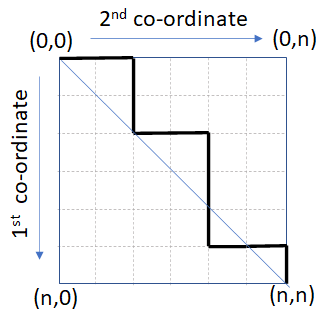
\includegraphics[width=0.4\linewidth]{images/sample-path.png}
    \caption{A path from $(0,0)$ to $(n,n)$ using downward and right edges}
    \label{fig:sample-path}
\end{figure}

If we represent each right move as $R$ and each downward move as $D$, one can observe that there's a bijection $f$ from the set of paths to set of strings of length $2n$ over the alphabet $\{D,R\}$ with number of $D$'s = number of $R$'s = $n$. Formally, if $(u_0,v_0), (u_1,v_1),\cdots,(u_{2n},v_{2n})$ represents the path where $(u_0,v_0)=(0,0)$ and $(u_{2n},v_{2n})=(n,n)$, and $b=b_1b_2\cdots b_{2n}$ represents the string where each $b_i$ is either $D$ or $R$, our bijection $f$ takes a path as input and sets $b_i$ as
$$b_i=\begin{cases}
D &\mbox{if } u_i = u_{i-1}+1\\
R &\mbox{if } v_i = v_{i-1}+1
\end{cases}$$
\begin{description}
\item \underline{Well defined:} As we have exactly $n$ $x$ co-ordinate increments and $n$ $y$ co-ordinate increments, we will have exactly $n$ $D$'s and $n$ $R$'s in our string and thus $f$ is well defined.
\item \underline{Injective:} Two different paths from $(0,0)$ to $(n,n)$ will different in at least one $(u_{i-1},v_{i-1})$ to $(u_i,v_i)$ transition where $i=1,2,\cdots,2n$, their corresponding strings under $f$ will differ in at least $i^{th}$ position and thus $f$ is injective.
\item \underline{Surjective:} Every string over $\{D,R\}$ of length $2n$ with equal number of $D$'s and $R$'s has a pre-image under $f$ which is defined by $(u_0,v_0)=(0,0)$ and $(u_i,v_i)$ is $(u_{i-1}+1,v_{i-1})$ if $b_i=R$ and $(u_{i-1},v_{i-1}+1)$ if $b_i=D$. As there will be $n$ $D$'s and $n$ $R$'s, $(u_{2n},v_{2n})=(n,n)$ and thus $f$ is surjective .
\end{description} 
Thus $f$ is bijection. As we have number of string over $\{D,R\}$ of length $2n$ with equal number of $D$'s and $R$'s equal to $\binom{2n}{n}$ (select $n$ positions out of $2n$ available and fill them with $D$'s and the rest with $R$'s). Thus the number of paths from $(0,0)$ to $(n,n)$ with only downward and rightward movements is $\binom{2n}{n}$.

Lets ask a slightly question. How many ways are there to go from $(0,0)$ to $(n+1,n-1)$ using only downward or right edges.Using a similar arguments as above, we can come up with a bijection to set of string over $\{D,R\}$ of length $2n$ with $n+1$ $D$'s and $n-1$ $R$'s. Therefore number of required paths are $\binom{2n}{n+1}=\binom{2n}{n-1}$

%\Lecture{Jayalal Sharma}{Sept 19, 2020}{07}{Catalan Bijections}{Anshu Yadav}{$\alpha$}{JS}

\subsection{Diagonal avoiding paths and Catlan numbers}
%Path coordinate Notation: 
In this section we explore the connection  between the above paths that we discussed and the Catalan number. 
Let us ask this question:
How many paths are there in the grid from $(0,0)$ to $(n,n)$ that avoids crossing the diagonal? 

We first define what \textit{crossing the diagonal} means. The diagonal consists of the points of the form $(i,i)$, $i\in\{0,\ldots, n\}$. A path $((u_0,v_0), \ldots, (u_{2n},v_{2n}))$ is said to be crossing the diagonal if it \textit{intersects} through the diagonal and goes to some point below the diagonal. Mathematically, a path is a diagonal crossing path if $\exists~i$ such that $u_i>v_i$. In particular, $\exists i: u_i = v_i+1$ (refer fig. \ref{fig:diagonal-crossing-path} for example. Any diagonal crossing path must necessarily pass through one of the red dots). Equivalently, in a diagonal avoiding path $\forall i\in\{0,\ldots, 2n\}, v_i\ge u_i$. A sample \emph{diagonal-avoiding path} is shown in the fig. \ref{fig:diagonal-avoiding-path} %\anote{explain $u_i = v_i+1$}
\begin{figure}[h!]
    \centering
    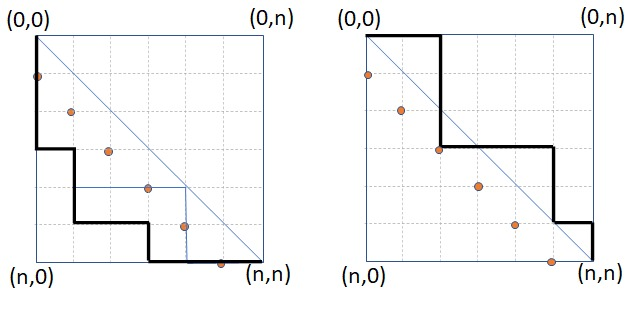
\includegraphics[width=0.7\linewidth]{images/diagonal-crossing.jpeg}
    \caption{Diagonal crossing paths. Note that path in (a) is crossing the diagonal at $(0,0)$}
    \label{fig:diagonal-crossing-path}
\end{figure}

\begin{figure}[h!]
    \centering
    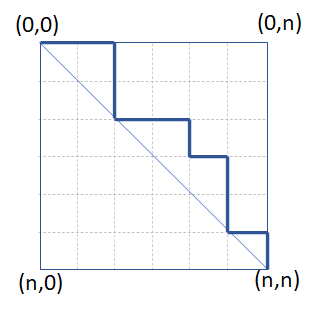
\includegraphics[width=0.4\linewidth]{images/diagonal-avoiding-path.png}
    \caption{A diagonal avoiding path. Observe that it can still touch the diagonal}
    \label{fig:diagonal-avoiding-path}
\end{figure}

Before computing this number, an obvious question is what is the connection between such restricted paths and Catalan number. It turns out that the set of diagonal avoiding paths from $(0,0)$ to $(n,n)$ is in bijection with the set of balanced paranthesized strings of length $2n$. Hence, to count the number of balanced paranthesized strings of length $2n$, which is also the Catalan number, we only need to count the diagonal avoiding paths from $(0,0)$ to $(n,n)$. Let us first establish the bijection between the two.

\subsection{Bijection from Diagonal avoiding paths to Balanced parenthesisation problem}
Intuitively, the bijection can be defined as follows: for any given balanced parenthesized string $w = w_1w_2\ldots w_{2n}$, the corresponding path from $(0,0)$ to $(n,n)$ is obtained by starting from position $(0,0)$, and scanning the string from left to right. Take  right move whenever $`('$ is encountered and a down move for $`)'$. Formally we define the bijection as follows:
\medskip{}

\noindent\underline{Defining the bijection:} Let $P$ be the set of diagonal avoiding paths from $(0,0)$ to $(n,n)$  and $B$ be the set of balanced paranthesized  strings of length $2n$ over the alphabets $\{(,)\}$. Define the bijection $\phi:B\rightarrow P$ as follows:\\
For $w=w_1 w_2 \ldots w_{2n}\in B$, $\phi(w) = (u_0,v_0), (u_1,v_1), \ldots, (u_i, v_i), \ldots, (u_{2n}, v_{2n})$, where 
\begin{enumerate}
    \item $(u_0,v_0)=(0,0)$ 
    \item $\forall i\in\{1,2,\ldots, 2n\}$\\
    \[
    (u_i, v_i) = 
    \begin{cases}  
    (u_{i-1}+1, v_{i-1})& ~~~~\text{if }w_i=)\\
    (u_{i-1}, v_{i-1}+1)&~~~~\text{if }w_i=(
    \end{cases}
    \]
    % $(u_i, v_i) = (u_{i-1}+1, v_{i-1})~~~~\text{if }w_i='('$\\
    % $(u_i, v_i) = (u_{i-1}, v_{i-1}+1)~~~~\text{if }w_i=')'$
\end{enumerate}
\underline{Proof of bijection}
\begin{description}
\item \textit{Well-defined:} From the above description, given any string $w$, $\phi(w)$ is uniquely defined. Further, for any string $w\in B$, since the number of $'('$ is same as  the number of $')' = n$, the corresponding path has $n$ right and $n$ down moves and hence it ends at $(n,n)$. Also, since the number of left brackets is greater than or equal to the number of right brackets in any prefix of $w$, for all $i\in[2n]$, $v_i\ge u_i$. This shows that $\forall w\in B, \phi(w)\in P$. Hence,  $\phi$ is well-defined.
\item \textit{Injective:} Let $w, w'$ be two different strings in set $B$. Then $\exists~$ an index $i\in[2n]$ where $w_i\ne w'_i$. Hence $\phi(w)$ and $\phi(w')$ also differ at the $i$th step, where one of the paths takes one step right while the other takes one step down. 
\item \textit{Surjective:} 
Given any path $((0,0), (u_1, v_1), \ldots, (u_{2n}, v_{2n}))$ the corresponding string $w\in B$ is defined as follows:\\
$\forall i\in[2n]$
\[
w_i = 
\begin{cases}
`(`& ~~~~~\text{if } (u_i, v_i) = (u_{i-1}, v_{i-1}+1)\\
`)`& ~~~~~\text{if } (u_i,v_i) = (u_{i-1}+1, v_{i-1})
\end{cases}
\]
We can verify that the string $w$ indeed is in set $B$, because firstly, for any path in $P$, $\forall i, v_i\ge u_i$ and hence by definition, number of left brackets $`(`$ in $w$ is greater than or equal to number of right brackets, $`(`$ in any prefix of $w$. Secondly, for any path to reach from $(0,0)$ to $(n,n)$ it must have $n$ right moves (increase in 2nd coordinate) and $n$ down moves (increase in 1st coordinate) and hence $w$ must have $n$ left brackets and $n$ right brackets.
\end{description}


% Properties:
% %$\phi(w_1)=u_1$ and $\phi(w_2)=u_2$ will be same till $(i-1)$th step, i.e. $(u_{1,(i-1)}, v_{1,(i-1)}=(u_{2,(i-1)}, v_{2,(i-1)}$ for $j=0$ to $i-1$.

\subsection{Counting the number of diagonal avoiding paths} 
Having established the bijection between Catalan number and diagonal avoiding paths, we get  
\begin{equation}
\label{eq:catalan-expr-1}
    C_n = \# \text{ of diagonal avoiding paths from } (0,0) to (n,n) 
\end{equation}
So, our next task is to count the number of diagonal avoiding paths from $(0,0)$ to $(n,n)$. 
To count this, we take following approach. Let us call the diagonal avoiding paths as \textit{good} paths and diagonal crossing paths as \textit{bad} paths. Then,
\begin{equation}
\label{eq:no-of-good-paths}
\Large
    \substack{\text{\# of diagonal avoiding paths }\\ \text{from } (0,0) \text{ to } (n,n)}  = \substack{\text{\# of paths }\\ \text{from } (0,0) \text{ to } (n,n)} - \substack{\text{\# of diagonal crossing paths }\\ \text{from } (0,0) \text{ to } (n,n)}
\end{equation}  

So, now our revised goal is to count the number of diagonal crossing paths from $(0,0)$ to $(n,n)$. How do we do that? Here again bijection plays an important role. The idea is to translate diagonal crossing paths into  different kind of paths which are easy to count. 

Let us define the following path translation:  Let $\pi=(0,0), (u_1,v_1), \ldots, (u_{2n}, v_{2n})$ be  a diagonal crossing path. Then there must exist $i$ such that $u_i = v_i+1$. There can be many such indices as the path can cross the diagonal multiple times. Choose $i$ to be the least such index. Let $u_i = \ell$, then the first co-ordinate after crossing the diagonal is $(\ell, \ell-1)$. Let us call this point $P$ (refer fig. \ref{fig:reflecting-path}(a)). Then to find the translated path we reflect the part of the path $\pi$ after point $P$ w.r.t. the main diagonal. 

\begin{figure}[h!]
    \centering
    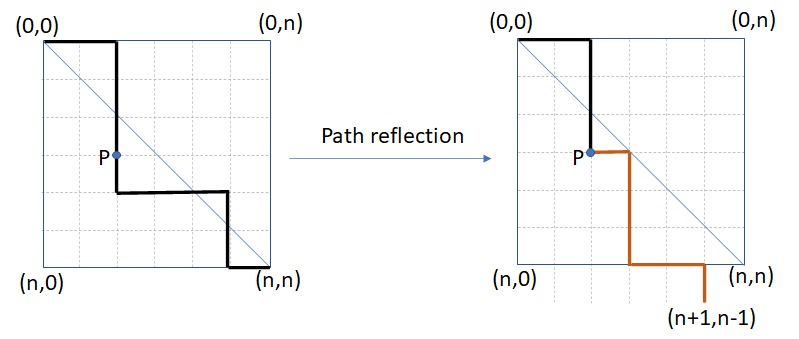
\includegraphics[width=0.7\linewidth]{images/reflecting-path.jpeg}
    \caption{Point P in a diagonal crossing path and the reflected path after P}
    \label{fig:reflecting-path}
\end{figure}

More precisely, we can divide the diagonal crossing path into two stretch $S_1, S_2$, where $S_1$ is the part of the path between $(0,0)$ to $P$ and $S_2$ is the part of the path between $P$  to $(n,n)$. 
Then to translate $\pi$ into a new path, replace $S_2$ with $S_2'$  to get a new path $\pi' = S_1S_2'$. The replacement $S_2'$ is defined as follows:
\begin{itemize}
    \item[-] replace downward edges with right edges and 
    \item[-] replace right edges with downward edges.
\end{itemize} Refer fig. \ref{fig:reflecting-path}(b)
We can observe that the new path $\pi'$ described in this way is always between $(0,0)$ to $(n+1, n-1)$. The argument for this goes as follows:

Originally (in $S_2$), $(\ell, \ell-1)$ goes to $(n,n)$ which means it takes $(n-\ell)$ downward moves and $(n-\ell+1)$ right moves. Since, we are swapping the right and downward moves to get $S_2'$ from $S_2$, there are $(n-\ell+1)$ downward moves and $(n-\ell)$ right moves from point $P=(\ell, \ell-1)$ in $S_2'$. Thus, $S_2'$ goes from $(\ell, \ell-1)$ to $(\ell+n-\ell+1, \ell-1+n-\ell) = (n+1, n-1)$ and hence, $\pi' = S_1S_2'$ is a path from $(0,0)$ to $(n+1, n-1)$. 

Thus we have established that any diagonal crossing path from $(0,0)$ to $(n,n)$ maps to a path from $(0,0)$ to $(n+1,n-1)$ after applying the transformation described above. The converse is also true, i.e., given any path from $(0,0)$ to $(n+1, n-1)$, we can translate it back to a diagonal crossing path from $(0,0)$ to $(n,n)$ by using the same reflection technique.  Thus, we get a bijection between the set of diagonal crossing paths from $(0,0)$ to $(n,n)$ to the set of paths from $(0,0)$ to $(n+1,n-1)$. We formally define the translation and prove that it is indeed a bijection.
\begin{description}
\item \underline{Bijection:}
Let $A$ be the set of diagonal crossing paths from $(0,0)$ to $(n,n)$ and $B$ be the set of paths from $(0,0)$ to $(n+1,n-1)$. Then the mapping $\phi:A\rightarrow B$ is formally defined as follows: 
\\
Let $\pi=(0,0), (u_1,v_1), \ldots, (u_{2n}, v_{2n})$ and $(u_i, v_i)$ be the first point when $\pi$ crosses the diagonal. Then $\phi(\pi) = \pi'=(0,0), (u'_1,v'_1), \ldots, (u'_{2n}, v'_{2n})$ is given by:
\begin{enumerate}
    \item $\forall 1\le j\le i, (u'_j, v'_j) = (u_j, v_j)$
    \item $\forall i+1\le j\le 2n$, 
    \[
    (u'_j, v'_j) = 
    \begin{cases}
    (u'_{j-1}+1, v'_{j-1})& ~~~~~\text{if } (u_j, v_j) = (u_{j-1}, v'_{j-1}+1)\\
    (u'_{j-1}, v'_{j-1}+1)& ~~~~~\text{if } (u_j, v_j) = (u_{j-1}+1, v'_{j-1})
    \end{cases}
    \]
\end{enumerate}
% We can verify that $\phi:A\rightarrow B$ satisfies all the properties of a bijection as follows:
\item \textit{Well-defined:} We already observed that any path $\pi\in A$ from $(0,0)$ to $(n,n)$ maps to a path $(0,0)$ to $(n+1,n-1)$. Hence $\phi$ is well defined.
\item \textit{Injection:} Consider two different diagonal crossing paths $\pi_1$ and $\pi_2$. Let $\pi_1 = S_{1,1}S_{1,2}$ and $\pi_2 = S_{2,1}S_{2,2}$, where the two components $S_{i,1}$ and $S_{i,2}$ for $i\in\{1,2\}$ are as defined before. Then following two cases are possible:
\begin{itemize}
    \item Case1: $S_{11}\ne S_{21}$. Then $\pi_1'\ne \pi_2'$, because the first component is copied as it is in the translation, i.e. $\pi_1' = S_{1,1}S_{1,2}'$ and $\pi_2' = S_{2,1}S_{2,2}'$.
    \item Case2: $S_{11}= S_{21}$, but $S_{12}\ne S_{22}$. In this case $S_{12}'\ne S_{22}'$ because of the way it is defined, i.e. for every right move there is a downwards move and vice-versa. Hence, $\pi_i'\ne \pi_2'$.
\end{itemize}
\item \textit{Surjective:} Given any path $\pi'$ from  $(0,0)$ to $(n+1,n-1)$, we can construct the corresponding path $\pi$ from $(0,0)$ to $(n,n)$, such that $\phi(\pi) = \pi'$, as follows.\\
Let $\pi'=(0,0), (u'_1,v'_1), \ldots, (u'_{2n}, v'_{2n})$. Since $\pi'$ goes to $(n+1, n-1)$ which is below the diagonal there must exist $i$ such that $(u'_i,v'_i)$ is below the diagonal. Again, there can be many such indices. Take $i$ to be the first such index. Same as before, let $\pi' = S_1'S_2'$, where $S_1'$ is the path from $(0,0)$ to $(u_i', v_i')$ and  $S_1'$ is the path from $(u_i',v_i')$ to $(u_{2n}', v_{2n}')$. Then $\pi = S_1'S_2$ where $S_2$ is obtained from $S_2'$ by swapping the right and downwards moves. Mathematically, let $\pi=(0,0), (u_1,v_1), \ldots, (u_{2n}, v_{2n})$. Then
\begin{enumerate}
    \item $\forall j\le i$, $(u_j, v_j) = (u_j', v_j')$
    \item $\forall~i+1\le j\le 2n$
    \[
    (u_j, v_j) =
    \begin{cases}
    (u_{j-1}+1, v_{j-1}) & ~~~~~\text{if } (u_j', v_j') = (u_{j-1}', v_{j-1}'+1)\\
    (u_{j-1}, v_{j-1}+1) & ~~~~~\text{if } (u_j', v_j') = (u_{j-1}'+1, v_{j-1}')
    \end{cases}
    \]
\end{enumerate}
Again by the same argument as before it can be verified that $\pi$ is a diagonal crossing path from $(0,0)$ to $(n,n)$. We write it here for completeness. Let $(\ell, \ell-1)$ be the first point when $\pi'$ crosses the diagonal. Then since the path from $(0,0)$ to $(\ell, \ell-1)$ remains as it is in $\pi$, it is a diagonal crossing path. Further since $\pi'$ is path from $(0,0)$ to $(n+1, n-1)$, it takes $n+1-\ell$ downward steps and $n-\ell$ right steps from $(\ell, \ell-1)$. Hence, $\pi$ takes $n+1-\ell$ right and $n-\ell$ downward steps from $(\ell, \ell-1)$. Thus, $\pi$ ends at $(\ell+n-\ell, \ell-1+n+1-\ell) = (n,n)$. 
\end{description}

Thus, we have established a bijection between the set of diagonal crossing paths from $(0,0)$ to $(n,n)$ and the set of  paths from $(0,0)$ to $(n+1,n-1)$. Hence, 
\begin{eqnarray*}
    \# \text{of diagonal crossing paths from } (0,0) \text{ to } (n,n) &=& \# \text{of paths from } (0,0) \text{ to } (n+1,n-1)\\
    &= &{2n\choose n+1}
\end{eqnarray*}
Hence, from~\eqref{eq:catalan-expr-1},\eqref{eq:no-of-good-paths},
\begin{align*} %\label{eq:no-of-good-paths-2}
C_n &= \# \text{of diagonal avoiding paths from} (0,0) \text{ to } (n,n)\\
%\Large
 %   \substack{\text{\# of diagonal avoiding paths }\\ \text{from } (0,0) \text{ to } (n,n)} 
     &= \Large \substack{\text{\# of paths }\\ \text{from } (0,0) \text{ to } (n,n)} - \Large\substack{\text{\# of diagonal crossing paths }\\ \text{from } (0,0) \text{ to } (n,n)}\\
    &= {2n\choose n} - {2n\choose n+1}\\
    & = {2n\choose n} - \frac{n}{n+1}{2n\choose n}\\
    &=\frac{1}{n+1}{2n\choose n}
\end{align*}  

Here, in the second last line, we have used the identity: $${2n\choose n+1} = \frac{n}{n+1}{2n\choose n}.$$









% Let us define the following path translation: Let $p=(0,0), (u_1,v_1), \ldots, (u_{2n}, v_{2n})$ be  a diagonal crossing path which goes below the diagonal at point $(u_i, v_i)$ for for the first time. Then, translate the path $p$ to a new path $p' = (u'_0, v'_0), (u'_1,v'_1), \ldots, (u'_{2n}, v'_{2n})$ by \textit{reflexing} $p$ between  $(u_i, v_i)$ and $(u_{2n}, v_{2n})$ in the sense that whenever $p$ goes right, $p'$ goes down, and whenever $p$ goes down, $p'$ moves right. Mathematically,
% \begin{enumerate}
%     \item $\forall 1\le j\le i, (u'_j, v'_j) = (u_j, v_j)$
%     \item $\forall i+1\le j\le 2n$, 
%     \[
%     (u'_j, v'_j) = 
%     \begin{cases}
%     (u'_{j-1}+1, v'_{j-1})& ~~~~~\text{if } (u_j, v_j) = (u_{j-1}, v'_{j-1}+1)\\
%     (u'_{j-1}, v'_{j-1}+1)& ~~~~~\text{if } (u_j, v_j) = (u_{j-1}+1, v'_{j-1})
%     \end{cases}
%     \]
% \end{enumerate}
% In the example, we can see that the translated path ends up at $(n+1, n-1)$. In general, we can prove the following: The above defined translation of any diagonal crossing path $p$ from $(0,0)$ to $(n,n)$ always ends at $(n+1, n-1)$.
% \begin{proof}
% Let $p$ croses the diagonal for the first time at $(u_i, v_i)$. Then 
% $$u_i = v_i+1.$$ 
% From $(u_i, v_i)$, $p$ moves $(n-u_i)$ steps down and $(n-v_i)$ steps in the right to reach $(n,n)$. Hence, the translated path $p'$ takes $(n-u_i)$ steps right and $(n-v_i)$ steps down from $(u_i, v_i)$ and ends at $$ (u_i+n-v_i, v_i+n-u_i) = (n+(u_i-v_i), n+(v_i-u_i)) = (n+1, n-1)$$. 
% \end{proof}

% Conversely, any path $p'$ from $(0,0)$ to $(n+1, n-1)$ can be mapped to a diagonal crossing path from $(0,0)$ to $(n,n)$. Intuitively, this can be done by again reflecting it  from the point $(u_i, v_i)$, where it crosses the diagonal for the first time. Note that such a point always exist because to reach the point $(n+1, n-1)$ $p'$ must cross the diagonal because $(n+1, n-1)$ is below the diagonal. Using the same argument as above, it can be shown that this translates $p'$ into a diagonal crossing path from $(0,0)$ to $(n,n)$.

% Thus, we get a bijection between the set of diagonal crossing paths from $(0,0)$ to $(n,n)$ and the set of paths from $(0,0)$ to $(n+1,n-1)$ defined formally as follows:\\

% Definition: Let $A$ be the set of diagonal crossing paths from $(0,0)$ to $(n,n)$ and $B$ be the set of paths from $(0,0)$ to $(n+1,n-1)$. Then a bijection $\phi:A\rightarrow B$ is defined as follows:

% For any path $p = (u_0, v_0), (u_1, v_1), \ldots, (u_{2n}, v_{2n})\in A$, let $(u_i, v_i)$ be the point where the path crosses the diagonal for the first time. That is, 
% \begin{enumerate}
%     \item $\forall j<i, v_j\ge u_j$, and
%     \item $u_i=v_i+1$
% \end{enumerate}
% Then $\phi(p)=p' = (u'_0, v'_0), (u'_1, v'_1), \ldots, (u'_{2n}, v'_{2n})$, where
% \begin{enumerate}
%     \item 
% \end{enumerate}
\begin{ex}
\item Try to establish a bijection between the set of different possible polygon triangulation in a polygon of $n+2$ nodes and the set of binary trees with $n$ internal nodes.

\textit{Hint: associate each internal node with a triangle in a triangulation. Then, each internal node will have degree three, which is the case for full binary tree, except for the leaves. Leaves will correspond to those triangles whose one of the edge is the boundary of the polygon.}
\end{ex}

 

\Lecture{Jayalal Sarma}{Sept 19, 2020}{07}{From Bijections to PIE}{Anshu Yadav}{$\alpha$}{JS}

\section{Introduction}
In this lecture, we will continue with the use of bijections and use it in formally proving the two identities that we discussed in class and then see their relationship to the Principal of Inclusion and Exclusion. 

\section{The Identities}
Recall that we proved following two identities in one of the discussion sessions
\begin{align}
     \sum_{k=0}^n (-1)^k{n\choose k} &= 0 \label{REV1}\\ 
     \sum_{k=0}^m (-1)^k{n\choose k} &= (-1)^m{n-1\choose m} \label{REV2}
\end{align}
In this section, we will see the proofs for the above equations is detail
\subsection{Proof for Eqn. \eqref{REV1}} \label{subsec:identity-even-odd-1}
$$\sum_{k=0}^n (-1)^k{n\choose k} = 0$$
\begin{proof}
    The LHS counts the number of even sized subsets of $[n]$ with positive sign and odd size subsets with negative sign. Then we proved the result using bijection between even sized and odd sized subsets of $[n]$. Hence, we get 0 on RHS. Let us formally define the bijection here.
    
    Let $E$ be the set of all even sized subsets of $[n]$ and $O$ be the set of all odd sized subsets of $[n]$. Then the bijection  $\phi_i:E\rightarrow O$ is defined with respect to an element $i\in[n]$ as follows.
    
    Let $X\subseteq [n]$, such that $|X|$ is even. Then 
    \[
        \phi_i(X) = 
        \begin{cases}
            X\setminus \{i\} & ~~~~~\text{ if } i\in X\\
            X\cup\{i\} & ~~~~~\text{ if } i\not\in X
        \end{cases}
    \]
    \underline{Proof of bijection:}
    \begin{description}
        \item \textit{Well-defined:} Given any even sized subset $X$, there are two possibilities: (i) $i\in X$, (ii) $i\not\in X$. In first case, $i$ is removed from $X$, hence its size reduces by one and becomes odd. In the second case, $i$ is added, hence the size of the subset increases by one and becomes odd. Hence, $\phi$ is well defined.
        \item \textit{Injective:} Let $X$ and $X'$ be two distinct subsets of $[n]$. Then $\exists j\in[n]$ such that $j$ is present in exactly one of the two subsets. Wlog, let $j\in X$ and $j\not\in X'$. Now, if $j\neq i$, then $j\in \phi(X)$ and $j\not\in \phi(X')$ and hence $\phi(X)\neq \phi(X')$. On the other hand, if $j=i$, then $j\not\in \phi(X)$ and $j\in \phi(X')$. Hence, $\phi(X)\neq \phi(X')$.  
        \item \textit{Surjective:} Let $Y\in O$ be an odd sized subset of $[n]$. From $Y$, we can recover $X$ such that $\phi(X) = Y$ by the same operation as in $\phi$. That is, 
        \[
        X= \begin{cases}
            Y\setminus \{i\} & ~~~~~\text{ if } i\in Y\\
            Y\cup\{i\} & ~~~~~\text{ if } i\not\in Y
        \end{cases}
        \]
        It can easily be verified that in both the cases, $X$ is an even sized subset of $[n]$.
    \end{description}
    This completes the proof.
\end{proof}
%
%
\subsection{Proof for Eqn. \eqref{REV2}} \label{subsec:identity-even-odd-2}
$$\sum_{k=0}^m (-1)^k{n\choose k} = {n-1\choose m}$$
\begin{proof}
Now we look at the second identity which is even more interesting. To prove this identity we use \emph{almost bijection} where the bijection is between a set and subset of another set.

In words, the identity to prove, can be described as
$$\Large\substack{\# \textrm{ of even sized subsets of  $[n]$}\\  \textrm{of size atmost $m$}} - \substack{\# \textrm{ of odd sized subsets of $[n]$} \\ \textrm{of size atmost $m$}} = (-1)^m{n-1\choose m}.$$ Clearly, there cannot be a bijection between the two sets (even sized subsets and odd sized subsets) in this case, since their difference is non-zero. This is where we use almost bijection.

We use following case analysis. 
\begin{description}
\item \underline{\textbf{Case1:} $m$ is even:} Then the identity to prove is:
\begin{equation} \label{eq:even-odd}
    \sum_{k=0}^m (-1)^k{n\choose k} = {n-1\choose m}
\end{equation}
This can be interpreted as 
\begin{equation} \label{eq:even-odd-1}
    \sum_{\substack{k=0,\\k\text{ is even}}}^m {n\choose k} -  \sum_{\substack{k=1,\\k\text{ is odd}}}^{m-1} {n\choose k} = {n-1\choose m}
\end{equation}
Let $E$ be the set of all the even sized subsets of $[n]$ of size at most $m$ and $O$ be the set of odd sized subsets of $[n]$ having size at most $m-1$. Then, Eqn.~\eqref{eq:even-odd-1} can intuitively interpreted as follows: there is a subset $E'\subseteq E$, such that $E'$ is in bijection with $O$ and $|E\setminus E'| = {n-1\choose m}$. Thus, we have three tasks at hand
\begin{itemize}
    \item identify the set $E'$, and
    \item define and prove the bijection between $E'$ and $O$.
    \item prove that $|E\setminus E'| = {n-1\choose m}$
\end{itemize}
\underline{Defining the set $E'$:} Set $E'$ is the union of two sets: 
$$E' = \{X\subseteq [n]: |X| \textrm{ is even and } |X|\le m-2\}\cup\{X\subseteq [n]: i\in X \textrm{ and } |X| = m\}$$
\underline{Defining the bijection:} The bijection $\phi:E'\rightarrow B$ is defined in the same way as we defined it for first identity. That is, for $X\in E'$,
\[
\phi(X) = 
\begin{cases}
X\setminus \{i\} & ~~~~~\text{ if } i\in X\\
X\cup\{i\} & ~~~~~\text{ if } i\not\in X
\end{cases}
\]
\underline{Proof of bijection}
\begin{description}
\item \textit{Well-defined:} Let $X\in E'$, then (i) if $|X|\le m-2$, then $|\phi(X)|$ is odd and $|\phi(X)|\le m-1$, (ii) if $|X| = m$, then $i\in X$, hence $\phi(X) = X\setminus \{i\}$. This implies $|\phi(X)| = m-1$. Thus, in both the cases $\phi(X)\in O$.
\item \textit{Injective:} Since, the function is same as in the previous case, the same argument for injectivity works.
\item \textit{Surjective:} Let $Y\in O$ be an odd sized subset of $[n]$. From $Y$, we can recover $X\in E'$ such that $\phi(X) = Y$ by the same operation as in $\phi$. That is, 
 \[
 X= 
 \begin{cases}
Y\setminus \{i\} & ~~~~~\text{ if } i\in Y\\
Y\cup\{i\} & ~~~~~\text{ if } i\not\in Y
 \end{cases}
 \]
 It can easily be verified that in both the cases, $|X|$ is even. 
 In first case, since $|Y|\le m-1, |X|\le m-2$, hence $X\in E'$. In second case, since $i\not\in Y$ and $|Y|\le m-1$, $|X|\le m$ and $i\in X$. Hence $X\in E'$, by definition.
\end{description}
This proves the bijection between $E'$ and $O$. 

\underline{Proof for: $|E\setminus E'| = {n-1\choose m}$}

From the above definitions, $E\setminus E' = \{X\subseteq [n]: |X| = m, i\not\in X\}$. This can be interpreted as $E\setminus E' = \{X\subseteq [n]\setminus \{i\}: |X| = m\}$. Hence, $|E\setminus E'| = {n-1\choose m}$.

\item \underline{\textbf{Case2:} $m$ is odd:} In this case the identity to prove is:
\begin{equation}
\label{eq:even-odd-3}
    \sum_{k=0}^m (-1)^k{n\choose k} = - {n-1\choose m}
\end{equation}
This can be interpreted as 
\begin{equation}
\label{eq:even-odd-2}
    \sum_{\substack{k=0,\\k\text{ is even}}}^{m-1} {n\choose k} -  \sum_{\substack{k=1,\\k\text{ is odd}}}^{m} {n\choose k} = -{n-1\choose m}
\end{equation}
Equivalently,
\begin{equation}
\label{eq:odd-even-1}
    \sum_{\substack{k=1,\\k\text{ is odd}}}^{m} {n\choose k} - \sum_{\substack{k=0,\\k\text{ is even}}}^{m-1} {n\choose k}  = {n-1\choose m}
\end{equation}
This time the set of odd sized subsets of $[n]$ of size at most $m$ is bigger than the even sized subsets of $[n]$ of size at most $m$.
The proof is same as that for the case of even $m$. 
Let $E$ be the set of all the even sized subsets of $[n]$ of size at most $m-1$ (since $m$ is odd) and $O$ be the set of odd sized subsets of $[n]$ having size at most $m$. Then~\eqref{eq:odd-even-1} can be interpreted as follows: there is a subset $O'\subseteq O$, such that $E$ is in bijection with $O'$ and $|O\setminus O'| = {n-1\choose m}$.
  
Thus, we have two task at hand
\begin{itemize}
    \item identify the set $O'$, and
    \item define and prove the bijection between $E$ and $O'$.
    \item prove that $|O\setminus O'| = {n-1\choose m}$
\end{itemize}
\underline{Defining the set $O'$:} Set $O'$ to be the union of two sets: 
$$O' = \{Y\subseteq [n]: |Y| \text{ is odd and } |Y|\le m-2\}\cup\{Y\subseteq [n]: i\in Y \text{ and } |Y| = m\}$$
\underline{Defining the bijection:} The bijection $\phi:E\rightarrow O'$ is defined in the same way as we defined it for first identity. That is, for $X\in E$,
\[
\phi(X) = 
\begin{cases}
X\setminus \{i\} & ~~~~~\text{ if } i\in X\\
X\cup\{i\} & ~~~~~\text{ if } i\not\in X
\end{cases}
\]
\underline{Proof of bijection}
\begin{description}
\item \textit{Well-defined:} Let $X\in E$, then $\phi(X)$ is of odd size because either an element is added or removed from $X$, which is of even size. Now, (i) if $i\in X$, then $\phi(X) = X\setminus\{i\}$. Hence, $|\phi(X)|\le m-2$ (because $|X|\le m-1$) which implies $\phi(X)\in O'$ (ii) if $i\not\in X$, then, $\phi(X) = X\cup \{i\}$. This implies $|\phi(X)| \le m$. But since, $i\in \phi(X)$, $\phi(X)\in O'$. This proves that $\phi$ is well- defined.
\item \textit{Injective:} Since, the function is same as in sub section~\ref{subsec:identity-even-odd-1}, the same argument for injectivity works.
\item \textit{Surjective:} Let $Y\in O'$ be an odd sized subset of $[n]$. From $Y$, we can recover $X\in E$ such that $\phi(X) = Y$ by the same operation as in $\phi$. That is, 
 \[
 X= 
 \begin{cases}
Y\setminus \{i\} & ~~~~~\text{ if } i\in Y\\
Y\cup\{i\} & ~~~~~\text{ if } i\not\in Y
 \end{cases}
 \]
 It can easily be verified that in both the cases, $|X|$ is even. 
 In first case, $|Y|\le m$ and hence $|X|\le m-1$. So, $X\in E$. In second case, since $i\not\in Y$, $|Y|\le m-2$ (by definition) and hence $|X|\le m-1$. Hence $X\in E$.
\end{description}
This proves the bijection between $E$ and $O'$. 

\underline{Proof for: $|O\setminus O'| = {n-1\choose m}$}\\
From the above definitions, $O\setminus O' = \{Y\subseteq [n]: |Y| = m, i\not\in Y\}$. This can be interpreted as $O\setminus O' = \{Y\subseteq [n]\setminus \{i\}: |Y| = m\}$. Hence, $|O\setminus O'| = {n-1\choose m}$.
\end{description}
This completes the proof
\end{proof}
This proves both the identities.
%%%%%%%%%%%%%%%%%%%%%%%%%%%%%%%%%%%%%%%%%%%%%%%%%%%%%%%%%%%%%%%%%%%%%%%%%%%%%
\section{Principle of Inclusion and Exclusion}
Suppose we are given $n$ sets $A_1, A_2, \ldots, A_n\subseteq G$, where $G$ is some ground set. We are interested in finding the size of $A= A_1\cup A_2\cup\ldots\cup A_n$. This is very abstract scenario and we will see specific examples later, but here we are going to see classic use of the above identities in deriving this number.

So, we are interested in finding $|A| = |A_1\cup A_2\cup\ldots\cup A_n|$. 

So, here is a thought process - 
Clearly, we can add the size of individual sets as 
$|A| = |A_1|+|A_2|+\ldots +|A_n|$, but this will over-count if there are some elements present in more than one sets. So, for that we need to subtract the double counting. For e.g. if $x\in A_1$ and $x\in A_2$, then it gets counted twice and to compensate for that we need to subtract $|A|=|A_1\cap A_2|$ and we might attempt $|A| = |A_1|+|A_2|+\ldots +|A_n| - \sum_{1\le i < j\le n}|A_i\cap A_j|$. But then, if $x$ is present in $A_1, A_2$ and $A_3$, the it is under-counted (added thrice and subtracted thrice). So, again we need to compensate for that by adding $\sum_{1\le i \le j\le k\le n}|A_i\cap A_j\cap A_k|$ in the above expression and this sequence goes on for any element being present in $k\le n$ sets and finally we get the expression for $|A|$  as follows
\begin{equation} \label{eq:pie-1}
    |A| = |A_1|+\cdots+|A_n|-\sum_{1\le i< j\le n}|A_i\cap A_j| +\sum_{1\le i<j<k}|A_i\cap A_j\cap A_k| -\cdots + (-1)^{n+1}|A_1\cap A_2\cap\cdots\cap A_n|
\end{equation}
For $n=2$, the above expression gives
$$|A| = |A_1|+|A_2|-|A_1\cap A_2|$$
which we all must have seen before and can easily prove using Venn diagram. 

In this section, we will formally prove the above expression for general $n$ using the two identities we proved in previous section.
\begin{proof}
Consider any $x\in A_1\cup A_2\cup\cdots\cup A_n$. Let $x$ appears in $k$ of the $A_i$'s. Then let us see how $x$ gets counted
\begin{itemize}
    \item[-] $|A_1|+|A_2|+\cdots +|A_n|$: counts $x$ $k$ times (added)
    \item[-] $\sum_{1\le i<j\le n}|A_i\cap A_j|$: counts $x$ ${k\choose 2}$ times (subtracted)
    \item[-] $\sum_{1\le i<j<k\le n}|A_i\cap A_j\cap A_k|$: counts $x$ ${k\choose 3}$ times (added) 
    \item[-] and so on $\ldots$
\end{itemize}
Notice that in terms involving intersection of more than $k$ sets, $x$ never appears.

Thus, 
\begin{eqnarray*} 
{\Large\substack{\# \text{of times $x$}\\ \text{gets counted}}} &=& k+{k\choose 2}-{k\choose 3}+\cdots +(-1)^{k+1}{k\choose k}\\
&=&-{k\choose 0}+{k\choose 1}+{k\choose 2}-{k\choose 3}+\cdots +(-1)^{k+1}{k\choose k}+{k\choose 0}\\
&=&-\sum_{i=0}^k(-1)^{i}{k\choose i}+{k\choose 0}\\
%&&\text{from~\eqref{eq:identity-1}, $\sum_{i=0}^k(-1)^k{k\choose i} = 0$}\\
&=&{k\choose 0} ~~~~~~~~~~~~~~~~~~~~~~~\text{from ~\eqref{REV1}}\\
&=& 1
\end{eqnarray*}
Thus, irrespective of the value of $k$, any element $x\in A_1\cup A_2\cup\cdots\cup A_n$ is counted exactly once. Hence, every $x\in A_1\cup A_2\cup\cdots\cup A_n$ is counted exactly once in RHS in~\eqref{eq:pie-1}.

This proves the PIE
\end{proof}
Now let us look at the application of second identity that we derived. This identity is used in deriving a version of PIE which appears very naturally in several context. Let us look at one such example.

PIE says that if we want to derive $|A_1\cup\A_2\cup\cdots\cup A_n|$, then the following expression does not give the correct count.
$$|A_1\cup\A_2\cup\cdots\cup A_n| = |A_1|+|\A_2|+\cdots+|A_n|$$ 
But we can ask, does this expression gives a lower or an upper bound? As we saw, this does over-counting, hence we can write
$$|A_1\cup\A_2\cup\cdots\cup A_n| \le |A_1|+|\A_2|+\cdots+|A_n|$$
Now, suppose we include the next component, i.e. $$|A_1|+|\A_2|+\cdots+|A_n|-\sum_{1\le i<j\le n}|A_i\cap A_j|$$
Again from PIE we know that this also does not give the correct count. But we ask the same question again - does it give any lower or upper bound. And as we saw that this term can do some over-subtraction and hence we can say that this expression gives the lower bound. That is, 
$$|A_1\cup\A_2\cup\cdots\cup A_n| \ge |A_1|+|\A_2|+\cdots+|A_n|-\sum_{1\le i<j\le n}|A_i\cap A_j|$$
Similarly, 
$$|A_1\cup\A_2\cup\cdots\cup A_n| \le |A_1|+|\A_2|+\cdots+|A_n|-\sum_{1\le i<j\le n}|A_i\cap A_j|+\sum_{1\le i<j<k\le n}|A_i\cap A_j\cap A_k|$$
and we continue like this. 

Let us now formally establish this observation. We use the same technique that we used in the proof of PIE. 

Let $x$ appears in $k$ of the sets in $A_1, A_2, \ldots, A_n$. Suppose we cut off the PIE after $m\le n$ sized intersections. Then 
\begin{eqnarray*} 
{\Large\substack{\# \text{of times $x$}\\ \text{gets counted}}} &=& {k\choose 1}-{k\choose 2}+\cdots+(-1)^{m+1}{k\choose m}\\
%&=&-{k\choose 0}+{k\choose 1}+{k\choose 2}-{k\choose 3}+\cdots +(-1)^{k+1}{k\choose k}+{k\choose 0}\\
&=&-\sum_{i=0}^m(-1)^{i}{k\choose i}+{k\choose 0}\\
%&&\text{from~\eqref{eq:identity-1}, $\sum_{i=0}^k(-1)^k{k\choose i} = 0$}\\
&=& 1+(-1)^{m+1}{k-1\choose m} ~~~~~~~~~~~~~~~~~~~~~~~\text{from ~\eqref{REV2}}
\end{eqnarray*}
Thus, $x$ is over counted or under counted depending on whether the second term on RHS is positive or negative. Let us analyze this for two cases.
\begin{description}
\item Case1: $k\le m$

Since, $x$ appears in only $k\le m$ sets and we are cutting down only after $m$, then this means that all possible intersections of this particular $x$ are added and subtracted and $x$ can not appear in any of the intersections of more than $k$ sets. Hence, $x$ is neither under counted nor over counted. In the expression, ${k-1\choose m} = 0$ Hence,
$$\# \text{of times $x$ is counted } = 1$$
\item Case2: $k>m$

In this case, $x$ can be under counted or over counted depending upon whether $m$ is even or odd.
If $m$ is odd then $x$ is over counted.

If $m$ is even then $x$ is under counted.
\end{description}
Notice that either all $x\in A_1\cup\A_2\cup\cdots\cup A_n$ are correctly counted or under counted or all $x$ are correctly counted or over counted based on the parity of $m$. Thus, whether a PIE cut down after $m$ intersections gives lower bound or upper bound depends only on the parity of $m$. This principle is also called the \emph{Bon Ferroni's inequality}. 
\begin{remark} 
    We used the equality in~\eqref{eq:even-odd} to prove PIE. We can actually do the other way round as well, i.e. we can use PIE to prove this equality too.
\end{remark}
This completes this lecture. In the next lecture we will look at some applications of PIE.

%\Lecture{Jayalal Sharma}{Sept 19, 2020}{08}{Live lecture discussion}{Anshu and Narasimha Sai }{$\alpha$}{JS}

\section{Discussions}

\paragraph{Bijection from Euler's problem to Binary Trees} As we have already established a bijection from set of balanced parenthesisations to set of full binary trees and established that number of full binary trees with $n$ internal nodes is the catlan number $C_n$, in this section, let's establish a bijection from the \emph{Euler's Problem} to set of full binary trees to establish that the solution to \emph{Euler's problem} is also catlan number $C_n$.

Lets recall \emph{Euler's problem} first. Consider a convex polygon with $n+2$ edges. Euler's problem is the number of ways of triangulating it (partition the polygon into triangles) by drawing non-crossing diagonals. (Refer fig. \ref{fig:Euler's-polygon}). We know that number of non-crossing diagonals in a polygon of $n+2$ edges is $n-1$ (proof follows from a simple induction) and from those $n-1$ non-crossing diagonals, we have our polygon partitioned into $n$ triangles. Let's associate each of the triangles with a vertex (green dots in the fig. \ref{fig:Euler's-polygon}). Observe that if two triangles share an edge, it must be one of the diagonals (no two triangles can share an edge because of non-crossing diagonals). Now, let's connect the vertices whose corresponding triangles share an edge. Any edge connecting two of these vertices crosses a diagonal. 
\begin{figure}[h!]
    \centering
    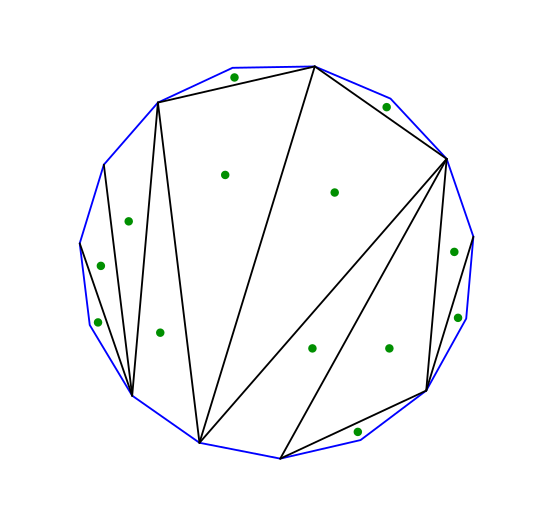
\includegraphics[width=0.4\linewidth]{images/polygon.png}
    \caption{Partitioning a polygon into triangles by non-crossing diagonals. Observe that green dots in each triangle associates the triangle with a vertex}
    \label{fig:Euler's-polygon}
\end{figure}
Now, consider a polygon edge $e$. For every polygon edge surrounding a vertex (other than $e$), add an open-edge originating from that vertex (see fig. \ref{fig:tree-in-polygon}). We arrive at the following claim.  
\begin{claim}
	If we remove the underlying triangles (which are formed with polygon edges and diagonals), from fig. \ref{fig:tree-in-polygon}, the 		resulting graph obtained (see fig. \ref{fig:tree}) is a full binary tree with the vertices as internal nodes.
\end{claim}
\begin{figure}[h!]
    \centering
    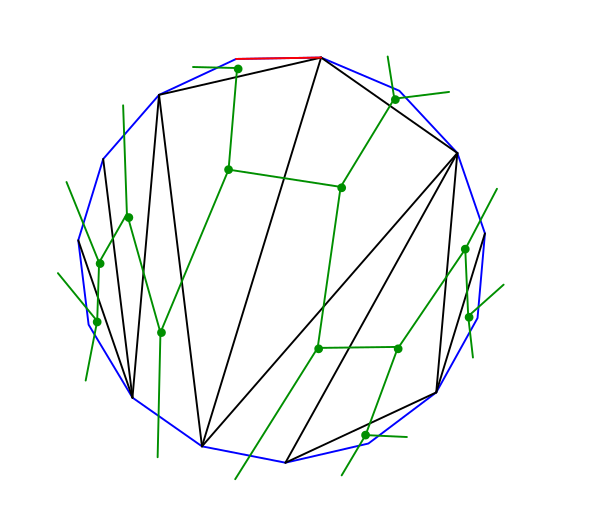
\includegraphics[width=0.4\linewidth]{images/polygon-tree.png}
    \caption{Polygon with vertices connected to form a tree}
    \label{fig:tree-in-polygon}
\end{figure}
\begin{figure}[h!]
    \centering
    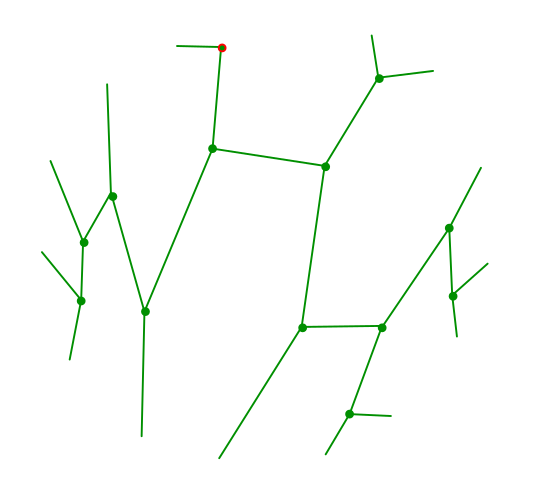
\includegraphics[width=0.4\linewidth]{images/tree.png}
    \caption{Tree formed by connecting vertices}
    \label{fig:tree}
\end{figure}
\begin{proof}
	We observe that degree of every vertex other than the vertex surrounded by edge $e$ is 2. This vertex will act as root to our full binary tree. All other vertices have degree 3 because each vertex is surrounded by a triangle and if a side is a diagonal, it will be connected to vertex which is surrounded by triangle that shares the diagonal and if the side is a polygon edge, then there will be an open edge corresponding to it originating from the vertex. Therefore the resulting graph formed is a full binary tree with our vertices as $n$ internal nodes and vertices corresponding to open edges are $n+1$ leaves (because there are $n+2$ edges and one edge is under consideration). This completes the description of bijection.
\end{proof}

We leave it as an exercise to the reader to prove that the mapping defined above is indeed a bijection.

\paragraph{Bijection from binary trees to full binary trees}
In this section we are interested in connection between binary and full binary trees. Recall that a full binary tree is one in which each node has either 0 or two children. On the other hand, when we say binary tree then it only means that each node can have at most two children. We want to find a bijection between set of binary trees with $n$ internal nodes and set of full binary trees with certain number of internal nodes. 

First of all lets try to see how to convert a given binary tree into a full binary tree so that we can reverse the process, i.e. recover the original (binary) tree back from the full binary tree without ambiguity. 

Here is the first attempt:

\noindent \underline{Attempt 1:} First natural approach can be to add a leaf node to all non-full (internal nodes having only one child) nodes, as shown in figure~\ref{fig:bt-fbt-attempt1}
\begin{figure}[h!]
    \centering
    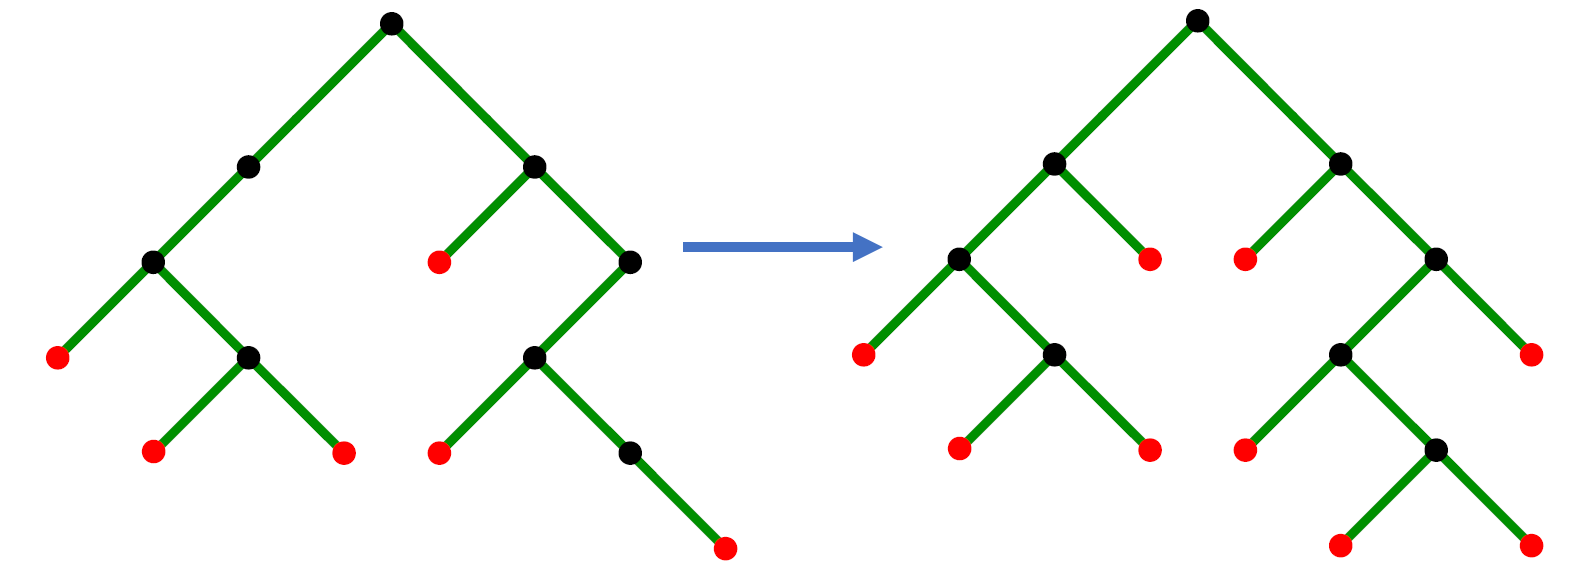
\includegraphics[width=0.7\linewidth]{images/binary-to-full-binary-1.png}
    \caption{Binary to full binary tree attempt1: adding a child node to each non full node}
    \label{fig:bt-fbt-attempt1}
\end{figure}

But notice that this transformation is not injective. For example, it can be observed that  both the trees in figure~\ref{fig:bt-fbt-attempt1-issue} map to same full binary tree.
\begin{figure}[h!]
    \centering
    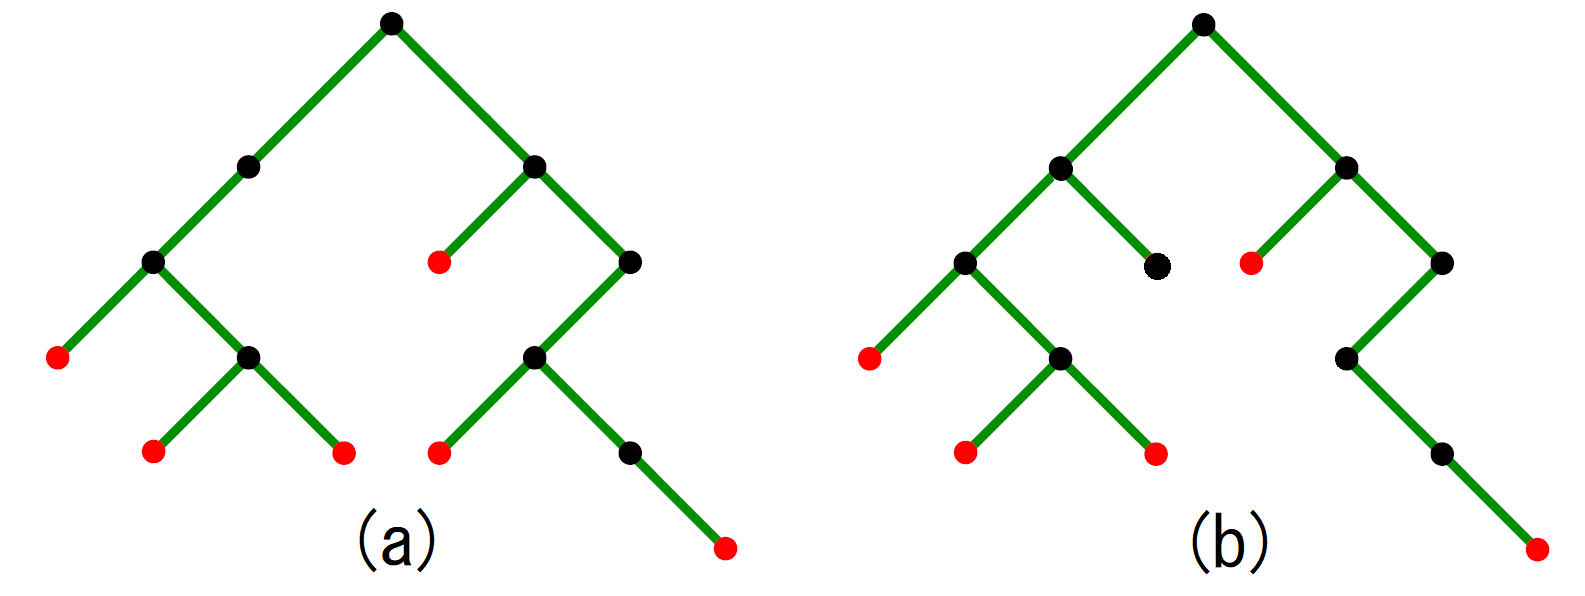
\includegraphics[width=0.7\linewidth]{images/binary-to-full-binary-2.png}
    \caption{Two different binary trees that map to same full binary tree}
    \label{fig:bt-fbt-attempt1-issue}
\end{figure}

\noindent\underline{Attempt 2(correct)}
Lets try a slightly different approach. Given a binary tree, do the following:
\begin{itemize}
    \item to each leaf node, add two children
    \item to each internal node having only one child, add another child
\end{itemize}
Figure~\ref{fig:binary-to-full-solution} shows the full binary tree constructed in this way for the same binary tree as in Figure~\ref{fig:bt-fbt-attempt1}.
\begin{figure}[h!]
    \centering
    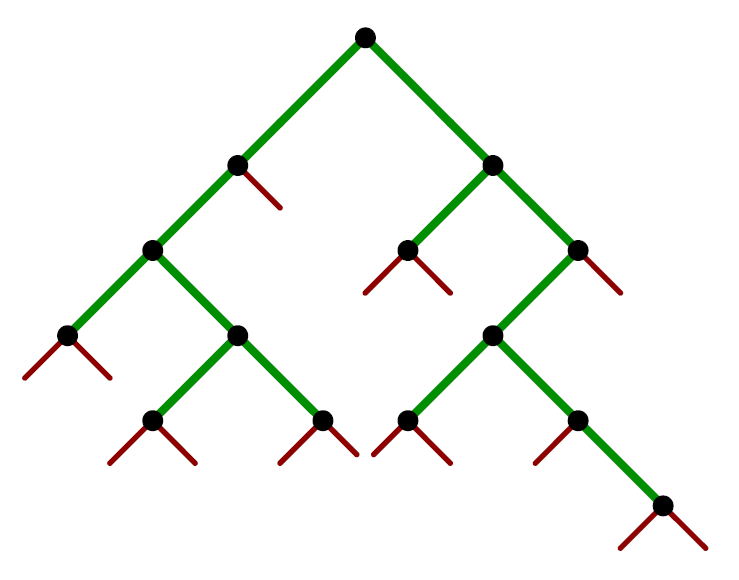
\includegraphics[width=0.5\linewidth]{images/full-binary-3.png}
    \caption{Full binary tree for the (non-full) binary tree given in fig~\ref{fig:bt-fbt-attempt1}. Notice that all the leaf nodes are added during transformation}
    \label{fig:binary-to-full-solution}
\end{figure}
We can see that this solution addresses the issue in the first attempt. Intuitively because of following argument: in the previous attempt the problem was that given a full binary tree, it was hard to decide if a leaf node was originally present in the binary tree or added during transformation. Now, in the current solution, this issue does not arise, because for any leaf node originally present in the binary tree, we add two new leaves as its children. Thus, it can be observed that all the leaf nodes (and only these nodes) are added during transformation.

To see that this translation is well-defined, we can see that the transformed tree is full binary tree by construction itself. Surjectivity is also easy to prove. To recover a binary tree from any given full binary tree, simply remove all the leaf nodes. We discussed injection informally. To give a formal argument, we first need to identify how to characterize two different binary trees? One of the hint as given during the discussion is to assign address to the nodes in the form of binary string, where 0-1 represents left or right child. 

Here we argued the bijection only intuitively and there are many things to be worked out formally. For example, proof for injection is not formally argued. Also, to argue surjection, we need to fix the number of nodes in full binary tree. Once we figure out this number, the argument for transformation being  well-defined also need to take that into account.

Writing a complete formal proof of bijection is left as homework exercise.

\paragraph{Bijection between plane trees and full binary trees}
A plane tree is a rooted tree with an ordering among the children. A plane tree can have more than two children. Figure~\ref{fig:plane-tree-1} shows a plane tree. 

\begin{figure}[h!]
    \centering
    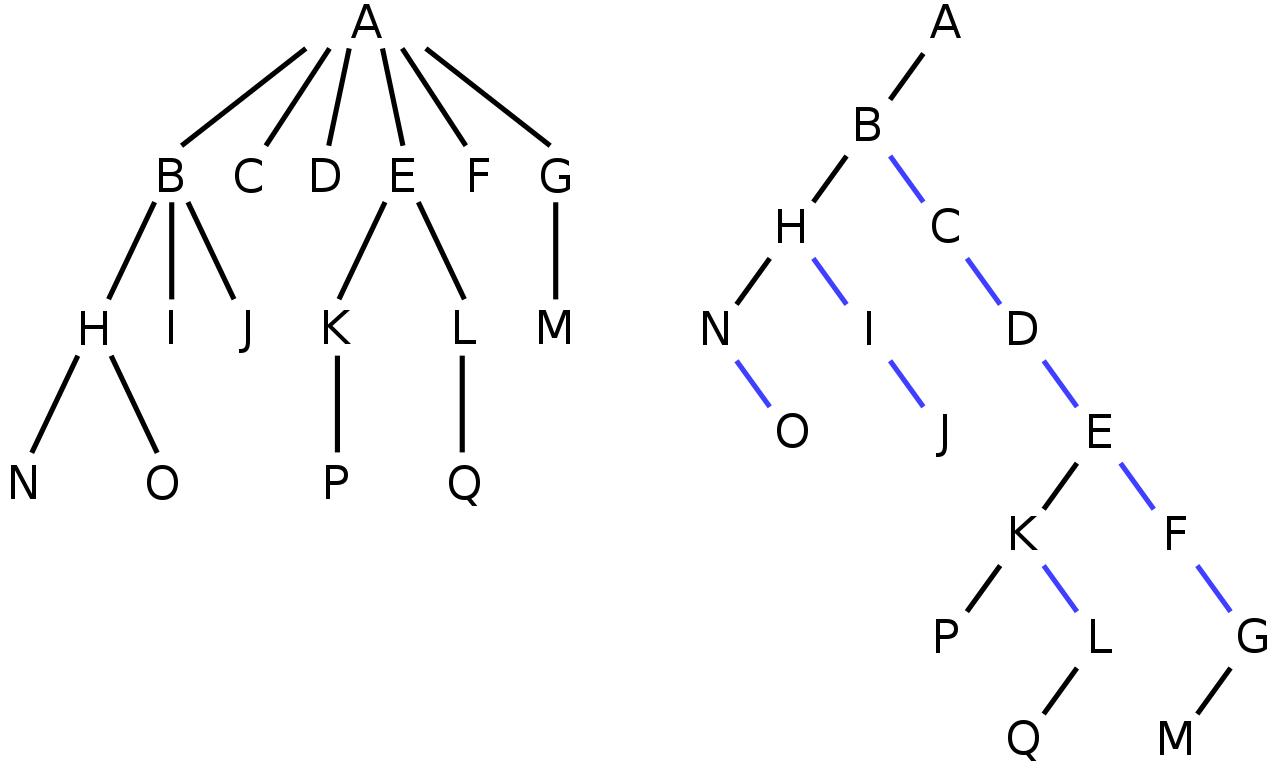
\includegraphics[width=0.8\linewidth]{images/plane-tree.png}
    \caption{An example of plane trees and its transformation to a binary tree}
    \label{fig:plane-tree-1}
\end{figure}

We are interested in studying the connection between plane trees and binary trees. The number of plane trees with $n$ nodes is equal to the number of binary trees with $n$ nodes. Thus, there is bijection between set of plane trees with $n$ nodes and the set of  binary trees with $n$ nodes. 

Here we define the bijection function. 

\noindent\underline{The Bijection:} Given any plane tree, do the following
\begin{itemize}
    \item For each node in the tree, 
    \begin{itemize}
        \item add its first child in plane tree as its left child in binary tree
        \item add its immediate sibling on right as its right child in binary tree.
    \end{itemize} child in the binary tree.
\end{itemize}
By following the above rule, we get a binary tree from given plane tree.

Observe that in the binary tree thus obtained, root node has only one child, while in general, in a binary tree the root can have both its children. Hence, we won't include the root as part of the binary tree.

Writing formal argument for all the properties is left as homework excercise.

\Lecture{Jayalal Sarma}{Sept 29, 2020}{08}{PIE and three applications}{Sumanth Naik}{$\alpha$}{JS}

%\section{Introduction}
The journey so far has been that we have been doing counting by bijections and established certain ideas regarding double counting and the bijections behind the scenes. Then we came to Principle of Inclusion-Exclusion(PIE) as a consequence of a bijection argument. In this lecture, we will look at another proof (an algebraic proof) for PIE and then 3 interesting applications of PIE.

\section{Principle of Inclusion Exclusion (PIE) - An Algebraic Proof} \label{sec:Principle of Inclusion - Exclusion(PIE)}
If there are $n$ subsets of a ground set $X$; $A_1$, $A_2$, $A_3, \ldots A_n$ $\subseteq$ $X$, then PIE helps us to estimate the size of the set of union of all $n$ subsets of the ground set. Mathematically, PIE states that,
\begin{align*}
\left|\bigcup_{i=1}^{n} A_i\right| &= \sum_{1 \le i \le n} | A_i|
\hspace{0.1cm}- \sum_{1 \le i < j \le n} \left| A_i \cap A_j \right| \\
&\hspace{0.5cm}+ \sum_{1 \le i < j < k \le n} | A_i \cap A_j \cap A_k| \hspace{0.2cm}.\hspace{0.1cm}.\hspace{0.1cm}.\hspace{0.1cm}.\hspace{0.1cm}.\\
\left|\bigcup_{i=1}^{n} A_i\right| &= \sum_{\emptyset \neq I \subseteq [n]} (-1)^{|I| +1} \left|\bigcap_{i \in I} A_i \right|\\
&=\sum_{\emptyset \neq I \subseteq [n]} (-1)^{|I| +1} \left|A_I\right|
\end{align*}
where $[n] = \{1,2,3, \ldots, n\} $ (short-hand notation for $1$ to $n$ elements) and $A_I = \bigcap_{i \in I} A_i$.\\
\\
Note that the intuition behind understanding the formula in the second step from first is that, $ \emptyset \neq I \subseteq [n]$ captures all the combinations of $1,2,3, \ldots ,n$ sized sets from $n$ sized set of numbers, i.e., $1 \le i \le n$ (set of combinations of 1 sized set from n sized set), $1 \le i < j \le n$ (set of combinations of 2 sized set from n sized set) and so on up to set of combinations of $n$ sized set from n sized set. The alternating sign in first equation's term is captured by $(-1)^{|I| +1}$ in second equation. And finally, the intersection part of all the terms in first equation, i.e., $|A_i|, |A_i \cap A_j|,  |A_i \cap A_j \cap A_j| \ldots$ is captured in $ \bigcap_{i \in I} A_i$ of the second equation.
\begin{proof}
Define the characterestic function of the set $A_i$ as $f_i$ described as : $f_i:X\longrightarrow\{0,1\}$, where the images are defined as $$\forall x \in X,\hspace{0.3cm} f_i(x) = 
  \begin{cases}
    1&\mbox{if } x \in A_i \\
    0& \textrm{otherwise }
  \end{cases}
$$

By definition, $(1-f_i(x))$ is the characteristic function for the compliment of $A_i$ (i.e. $X\setminus A_i$ or $\overline A_i$). In other words, when you subtract the characteristic function of a set from $1$, the difference is the characteristic function of the compliment of the same set. It is also to be noted that $f_i(x)f_j(x)$ is the characteristic function of $A_i\cap A_j$. In other words; when you multiply the characteristic functions of two sets with each other, the product is the characteristic function of the intersection of the two sets. 
\begin{align}
\intertext{Consider a function defined as,} F(x) &= \prod_{i=1}^{n}(1-f_i(x))\nonumber \\
&= (1-f_1(x))(1-f_2(x)) \ldots (1-f_n(x))\nonumber  \\
&= \sum_{I\subseteq[n]}(-1)^{|I|}\left(\prod_{i \in I} f_i(x)\right) \label{eq:F_def_in_PIE}
\end{align}
Note that the $F(x)$ represents the characteristic function of intersection of compliments (compliment of each $f_i$), hence by De-Morgan's Law, its mathematical equivalent is,
\[
\overline{\left(\bigcup_{i=1}^{n} A_i\right)} = X \setminus \bigcup	_{i=1}^{n}A_i
\]
To get the size of the set in the $RHS$ of previous equation (it has all the elements which are not present in any of the $n$ subsets of $X$), we just need to count the number of $x$'s in $X$ for which $F(x)$ is 1 (as $F(x)$ will be 1 for any $x$ only if every $f_i(x)$ is 0, i.e., $\forall i,x \notin A_i$). Hence:
\begin{equation}
\label{eq:sigma_F_1}
|X \setminus \bigcup_{i=1}^{n}A_i| = \sum_{x \in X} F(x) 
\end{equation}

Also from (\ref{eq:F_def_in_PIE}),
\begin{align}
\sum_{x \in X} F(x)&= \sum_{x} \sum_{I \subseteq [n]} (-1)^{|I|} \left(\prod_{i \in I} f_i(x)\right)\nonumber \\
&= \sum_{I \subseteq [n]} (-1)^{|I|} \left(\sum_{x} \left(\prod_{i \in I} f_i(x)\right)\right)\nonumber \\
&=\sum_{I \subseteq [n]} (-1)^{|I|} \left|\bigcap_{i \in I}A_i\right|\label{eq:sigma_F_2}
\end{align}
The last step is because $(\prod_{i \in I} f_i(x))$ is the characteristic function of intersection of $n$ subsets, i.e., $\bigcap_{i \in I}A_i$. And its summation over $x$, $(\sum_{x} (\prod_{i \in I} f_i(x)))$ will give us the size of the intersection, $\left|\bigcap_{i \in I}A_i\right|$. Also, note that the convention when $I=\emptyset$ is,
%\begin{equation}
$\left|\bigcap_{i \in I}A_i\right| = |X|$.
which can be reasoned as when $I$ is empty, $\left(\prod_{i \in I} f_i(x)\right)$ is $1$ for any $x$. And its summation over $x$, $\sum_{x} \left(\prod_{i \in I} f_i(x)\right)$ gives $|X|$.
\begin{align*}
\intertext{By (\ref{eq:sigma_F_1}) and (\ref{eq:sigma_F_2}),}
\left|X \setminus \bigcup_{i=1}^{n}A_i\right| &= \sum_{I \subseteq [n]} (-1)^{|I|} \left|\bigcap_{i \in I}A_i\right|\\
|X | - \left| \bigcup_{i=1}^{n}A_i\right| &= \sum_{I \subseteq [n]} (-1)^{|I|} \left|\bigcap_{i \in I}A_i \right|\\
\left| \bigcup_{i=1}^{n}A_i \right| &= |X| - \sum_{I \subseteq [n]} (-1)^{|I|} \left|\bigcap_{i \in I}A_i\right|\\ 
&=\sum_{\emptyset \neq I \subseteq [n]} (-1)^{|I|+1} \left|\bigcap_{i \in I}A_i \right| \\
\end{align*}
This completes the algebraic proof for PIE.
\end{proof}


\section{Applications of PIE} \label{sec:Applications of PIE - lec1}

We now see three different applications of PIE which exposes some interesting features of the tool.

\subsection{Counting the number of derangements on $n$ elements.} \label{subsec:derangements application}
Consider a scenario where, $n$ people go to a theatre to watch a movie, they keep their hats outside with the gatekeeper. On return, in a rush, the gatekeeper panicked and gave back the hats randomly.\\
\textbf{Question:} What is the chance that nobody got their own hat for a very large $n$?\\
\textbf{Answer (surprisingly high)}: roughly 36\% ! (more precisely, the probability is $1/e = 0.3678$).

Formally, if we view the rearrangement as a permutation on $n$ elements, the property that we are looking for can be expressed mathematically as follows : A permutation $\sigma \in S_n$ is said to be a derangement if $\forall i \in [n], \sigma(i) \ne i$.
Now we prove the following theorem.

\begin{theorem}
Number of derangements on $n$ elements is $$\left(\sum_{k=0}^{n} \frac{(-1)^k}{k!}\right)n!$$
\end{theorem}

Before we proceed, let us demonstrate why this implies our surprising answer. We know that the total number of ways for the $n$ people to pick $n$ hats is $n!$ (factorial of $n$) and hence the chance of derangement is $\left(\sum_{k=0}^{n} \frac{(-1)^k}{k!}\right)$. As $n\rightarrow\infty$, $\left(\sum_{k=0}^{n} \frac{(-1)^k}{k!}\right) \rightarrow 1/e \thicksim 0.3678$.). We now proceed with the proof of the above theorem, which is a nice application of PIE.

\begin{proof}
Let $S_n$ be the set of permutations on $n$ elements. $\sigma \in S_n$ is a permutation function on $n$  elements ($\sigma : [n] \rightarrow [n]$). $\forall_{i=1}^{n},~ \sigma(i)$ is defined as the person to whom $i^{\text{th}}$ person's hat was given. If $\sigma(i) = i$, then it means that the $i^{\text{th}}$ person got the correct hat - in terms of formal language of permutations, this is called a \textit{fix-point} of the permutation. What we are looking for is to count the number of fix-point-free permutations in $S_n$. 


The strategy is to count the number of non-derangements and subtract from $n!$.
Mathematically, non-derangement is captured as $\exists i,\hspace{0.2cm} \sigma(i) = i$. Now we set up the application of PIE in this context, by defining the $A_i$s first. Define $A_i$ as, 
$$\forall i \in \{1,2,...n\},\hspace{0.2cm} A_i = \{\sigma \in S_n\hspace{0.1cm} |\hspace{0.1cm} \sigma(i) = i\}$$ 
So, $A_i$ represents the set of $n$ elements whose $i^{\text{th}}$ element is fixed to $i$, other elements can be any non repeating value of $1$ to $n$ (except $i$ as it is taken).

The set that we want to estimate the size of - the set of non-derangement can be represented as $\bigcup_{i=1}^{n} A_i$.
Hence, we are interested in finding the number of non-derangements $|\bigcup_{i=1}^{n} A_i|$.

We want to apply PIE - which is about intersection of these $A_i$. Can $A_i$ and $A_j$ really intersect? Indeed, they can, and we can even estimate the size of the intersection: indeed, for a permutation to be in the intersection it has to be fixing the element $i$ and $j$ and it has the freedom to choose any permutation for the remaining values. Hence,
$$|A_i \cap A_j| = (n-2)!$$

Now we generalize this estimate to arbitrary size intersections since they appear in the RHS of PIE. For a shorthand notation, define, $A_I = \bigcap_{i \in I} A_i$. Now, from the statement of $PIE$, we need to estimate sizes of $\left| A_I \right|$ for different $I \subseteq [n]$. Observe that,
\begin{align}
|A_I| &= (n-|I|)! \label{eq:size_of_A_I_derangement_problem}
\end{align}
Indeed, in $A_I$, $\forall i \in I$, $\sigma(i)$ is fixed to $i$ by definition. For the remaining $n-|I|$ values, $\sigma$ can take any arbitrary permutation of the same $n-|I|$ values, hence $(n-|I|)!$ gives the number of possibilities.\\

Using PIE and using the idea of fixing size of $I$ and sum over each size in next step,
\begin{align}
|\bigcup_{i=1}^{n} A_i| &= \sum_{\emptyset \neq I \subseteq [n]} (-1)^{|I|+1} |A_I|\nonumber \\
&= \sum_{k=1}^{n} (-1)^{k+1} \left(\sum_{I\subseteq [n],|I|=k} |A_I|\right)\nonumber \\
&= \sum_{k=1}^{n} (-1)^{k+1} \left(\sum_{I\subseteq [n],|I|=k} (n-k)!\right)\nonumber \tag{By (\ref{eq:size_of_A_I_derangement_problem})}\\
&= \sum_{k=1}^{n} (-1)^{k+1} (n-k)! {n \choose k}\nonumber \\
&= \sum_{k=1}^{n} (-1)^{k+1} \frac{n!} {k!}\nonumber \\
&=  \left(\sum_{k=1}^{n}  \frac{(-1)^{k+1}} {k!}\right)n! \label{eq:non_derangements}
\end{align}
Now, to get number of derangements, subtract (\ref{eq:non_derangements}) from $n!$, which is 
\begin{align*}
n! - \left(\sum_{k=1}^{n}  \frac{(-1)^{k+1}} {k!}\right)n! &= \left(\sum_{k=0}^{n} \frac{(-1)^k}{k!}\right)n!
\end{align*}
\end{proof}

\subsection{Euler's $\Phi$ function.} \label{subsec:euler's function application}
\begin{theorem}
Let $n \in N$, $\Phi (n)$ = number of numbers $\leq n$, which are relatively prime to $n$. If $$n=\prod_{i=1}^{k}p_i^{\alpha_i}$$ where $p_i$ are distinct primes and $\forall i,~ \alpha_i \geq 1$, then $$\Phi(n) = n \left(\prod_{i=1}^{k}\left(1-\frac{1}{p_i}\right) \right)$$
\end{theorem}
\begin{proof}
Let $X=\{1,2,3,...,n\}$. Then,
\[
\forall 1 \leq i \leq k, A_i = \{m\in X ~|~p_i \textrm{ divides } m\}
\]
Thus, $A_i$ represents the set of multiples of $p_i$ less than $n$.
Number of numbers which are not relatively prime to $n$ is given by (as every number in any of $A_i$ will have $p_i$ as common factor) - is given by exactly the set : $\bigcup_{i=1}^{k} A_i$.  Thus we have the ground set for application for PIE. We need to be able to estimate the sizes of the intersections. More precisely:
\begin{align}
\Phi (n) &= n - |\bigcup_{i=1}^{k}A_i| \tag{apply PIE}
\nonumber \\
&=n- \sum_{I \subseteq [k], I \neq \emptyset} (-1)^{|I|+1}|A_I| \label{eq:mobius_with_PIE}
\end{align}
where
%\begin{align}
To esteimate $|A_I|$. We claim that $|A_I| = |\bigcap_{i \in I}A_i| = \frac{n}{\prod_{i \in I}p_i}$. This can be reasoned as follows : in $\bigcap_{i \in I}A_i$, there will be those numbers which are multiples of all the $p_i$'s. The same set can be obtained by including the product of every $p_i$, i.e., $\prod_{i \in I}p_i$, and all the numbers less than $n$ which are multiples of that product. The number of such numbers can be captured by $\frac{n}{\prod_{i \in I}p_i}$.\\
By Equation~\ref{eq:mobius_with_PIE} and using the convention of $\prod_{i \in I}p_i$ is 1 when $I=\emptyset$, 
\begin{align*}
\Phi (n) &= n - \sum_{I \subseteq [k], I \neq \emptyset} (-1)^{|I|+1}\frac{n}{\left(\prod_{i \in I}p_i\right)}\\
&= \sum_{I \subseteq [k]} (-1)^{|I|}\frac{n}{(\prod_{i \in I}p_i)}\\
&= n\sum_{I \subseteq [k]} (-1)^{|I|}\frac{1}{\left(\prod_{i \in I}p_i\right()}\\
&=n\left(\prod_{i=1}^{k}\left(1-\frac{1}{p_i}\right)\right)
\end{align*}
Note that the last step is done similar to  (\ref{eq:F_def_in_PIE}) in PIE (section \ref{sec:Principle of Inclusion - Exclusion(PIE)}) derivation : $f_i$ there is equivalent to $\frac{1}{p_i}$ here. This completes the proof for the theorem.
\end{proof}
\vspace{.5cm}
\noindent
\begin{corollary}$\Phi$ is multiplicative when numbers are co-primes. i.e., if $n_1, n_2$ are co-primes, then $\Phi(n_1 n_2) = \Phi(n_1) \Phi(n_2)$.
\end{corollary}
\begin{proof}
Let $A$ be the set of prime factors of $n_1n_2$. Since $n_1n_2$ is the product of two numbers $n_1$ and $n_2$, any prime $p \in A$ should divide at least one of $n_1$ and $n_2$. If $n_1$ and $n_2$ are co-primes, then the do not have any common prime factor. Therefore, any prime $p \in A$ should divide exactly one of $n_1$ and $n_2$. So, we can partition the set $A$ into two sets $X$ and $Y$ where $X$ is the set of prime factors of $n_1$ and $Y$ is that of $n_2$.
\begin{align*}
    \Phi(n_1n_2) &= n_1 n_2  (\prod_{p \in A}(1-\frac{1}{p}))\\
    &= n_1 (\prod_{p\in X}(1-\frac{1}{p})). n_2 (\prod_{p\in Y}(1-\frac{1}{p}))\\
    &= \Phi(n_1) \Phi(n_2)
\end{align*}
Thus, if $n_1$, $n_2$ are co-primes, then $\Phi(n_1 n_2) = \Phi(n_1) \Phi(n_2)$. \end{proof}


\subsection{Probability that two natural numbers are co-primes} \label{subsec:co-primes application}
For two randomly chosen natural numbers, what is the probability that they do not have a common factor (other than 1)?\\
Answer: $\sim60\% $
\begin{proof}
Fix $n$; $S = \{(a,b) | a,b \in [n]\}$.\\
Consider two definitions, the good set $G$ (represents set of pairs whose elements have $gcd = 1$) and the bad set $B$ (represents set of pairs whose elements have $gcd > 1$),
\[
G = \{(a,b)| \text{ no } d > 1 \text{ exist such that }d  \hspace{0.1cm}divides \hspace{0.1cm} a \text{ and } d  \hspace{0.1cm}divides \hspace{0.1cm} b\}
\]
\[
B = \{(a,b)| \exists d > 1 \text{ such that }d \hspace{0.1cm}divides \hspace{0.1cm} a \text{ and } d \hspace{0.1cm}divides \hspace{0.1cm} b\}
\]
We want the upper bound of $|B|$ in terms of $n^2$.\\
Define $X$ which has all the permutations of pairs possible as, $$X = \{(a,b)|a,b \in [n]\}$$
And for prime $p \le n$, define $A_p$ as a set which contains pairs whose elements both have $p$ as a prime factor and the pair belongs to $X$. $$A_p = \{(a,b)|p \hspace{0.1cm}divides \hspace{0.1cm}a,p \hspace{0.1cm}divides \hspace{0.1cm}b, p \hspace{0.1cm}is\hspace{0.1cm}prime ,(a,b)\in X\}$$
Clearly, $$B = \bigcup_{p \le n} A_p$$
By PIE, 
\begin{align}
|B| = \sum_{I \subseteq Q, I \neq \emptyset} (-1)^{|I|+1} |A_I| ~~\text{where,} ~~Q = \{p|p \le n, prime\}\label{eq:PIE_usage_application_3}
\end{align}
Now, the aim is to estimate $|A_I|$ (as stated in PIE), we can write,
\begin{align}
|A_I| =|\bigcap_{p_i \in I} A_{p_i}|\label{eq:size_of_A_I_mobius}
\end{align}
Here, $\bigcap_{p_i \in I} A_{p_i}$ denotes the set of pairs whose elements are both divisible by product of numbers (which are primes) in $I$. Note that the product need not be a prime. We can not write the resulting set ($\bigcap_{p_i \in I} A_{p_i}$) in terms of $A_p$ as $p$ is prime in the definition. So, lets create a new definition.\\
Let's define $A_d$, which denotes the set of pairs whose elements both have $d$ as a factor and the pairs belongs to $X$ (note that this definition is different from $A_p$ as there $p$ should be a prime, here $d$ can be any number), $$A_d = \{(a,b)|d \hspace{0.1cm}divides \hspace{0.1cm} a, d \hspace{0.1cm}divides \hspace{0.1cm} b, (a,b) \in X\}$$
Rewriting (\ref{eq:size_of_A_I_mobius}) using the definition of $A_d$,
\begin{align}
|A_I| =|A_d| \label{eq:size_of_A_I_equals_size_of_A_d}
~~where, \hspace{0.3cm}d = \prod_{p_i \in I}p_i
\end{align}
Estimating $|A_d|$ separately, from definition, $a$ can be any mutiple of $d$ which is less than or equal to $n$, similarly $b$ too can be any mutiple of $d$ which is less than or equal to $n$. Hence, 
\begin{align}
|A_d| &=\lfloor \frac{n}{d} \rfloor \lfloor \frac{n}{d} \rfloor\nonumber\\
&=(\lfloor \frac{n}{d} \rfloor)^2 \label{eq:size_of_A_d}
\end{align}
From (\ref{eq:PIE_usage_application_3}), splitting the summation by number of primes taking part, 
\begin{align}
|B| &=\sum_{k \geq 1} (\sum_{I \subseteq Q, I \neq \emptyset,|I| = k} (-1)^{|I|+1} |A_I|) \nonumber \tag{Apply (\ref{eq:size_of_A_I_equals_size_of_A_d}) and (\ref{eq:size_of_A_d}) }\\
&=  \sum_{k \geq 1}(\sum_{d \le n,\substack{d\text{ is a product } \\ \text{of } k \text{ distinct}\\ \text{primes from }Q} }(-1)^{k+1}(\lfloor \frac{n}{d} \rfloor)^2)  \label{eq:bad_set}
\end{align}
Note that the value of $k$ is used only to determine the sign of the terms in $|B|$. Usage of Mobius function gives a clever way to reduce the equation of $|B|$ to a single summation from double summation.\\
Mobius function $\mu(d)$ is given by
\[
  \mu(d) = 
  \begin{cases}
    0 &\mbox{if } p^2 \hspace{0.1cm} \text{divides} \hspace{0.1cm} d, \hspace{0.1cm} p  \hspace{0.1cm} \text{is prime}\\
    1 &\mbox{if } d = 1\\
    (-1)^k &\mbox{if } d \text{ is a product of }k \text{ distinct primes} 
  \end{cases}
\]
Using $\mu(d)$ in (\ref{eq:bad_set}),
$$|B| = \sum_{2 \le d \le n}(-\mu(d) ((\lfloor \frac{n}{d} \rfloor)^2))$$
Now estimating $|G|$; since all of $S$ can be either in $G$ or $B$ but not both and size of $S$ is $n^2$,
\begin{align}
|G| &= n^2 - |B|\nonumber \\
&= n^2 + \sum_{2 \le d \le n}\mu(d) ((\lfloor \frac{n}{d} \rfloor)^2)\nonumber \\
&= \sum_{1 \le d \le n}\mu(d) ((\lfloor \frac{n}{d} \rfloor)^2) \label{eq:good_set_1}
\end{align}
Last step uses the fact that $\mu(1) = 1$ in the Mobius function.\\
 Furthermore for any $x$,
\begin{align*}
(\lfloor x \rfloor )^2 - x^2 &= (x-\{x\})^2 - x^2\\
&= x^2 - 2\{x\}x + \{x\}^2 -x^2\\
&= -2x\{x\} + \{x\}^2\\
&= O(x)
\end{align*}
Using this fact in (\ref{eq:good_set_1}),
\begin{align}
|G| &= \sum_{1 \le d \le n}\mu(d) (\frac{n^2}{d^2} + O(\frac{n}{d}))\nonumber \\
&= n^2 \sum_{1 \le d \le n}\frac{\mu(d)}{d^2} +  O(n \sum_{1 \le d \le n}(\frac{\mu(d)}{d})) \label{eq:good_set_2}
\end{align}
Estimating the second term in (\ref{eq:good_set_2}): 
\begin{align}
n \sum_{1 \le d \le n}(\frac{\mu(d)}{d}) &\le n (\sum_{1 \le d \le n}\frac{1}{d})\nonumber \\
&\le n \log{n} \label{eq:term_2_in_good_set}
\end{align}
Last step is derived by the asymptotic estimate of the sequence of Harmonic series. \\ \\
Estimating the first term in (\ref{eq:good_set_2}):\\
Using Euler's series, the following approximation can be done.
\begin{align}
M = \sum_{d=1}^{\infty} \frac{\mu(d)}{d^2} \sim \frac{6}{\pi^2} \label{eq:approx_M}
\end{align} \\
It can also be proven that
\begin{align}
|M-\sum_{1 \le d \le n} \frac{\mu(d)}{d^2}| \le \frac{1}{n}\label{eq:term_1_in_good_set}
\end{align}
Using (\ref{eq:good_set_2}), (\ref{eq:term_2_in_good_set}), (\ref{eq:approx_M}) and (\ref{eq:term_1_in_good_set}),
\begin{align*}
|G| &= n^2 (\frac{6}{\pi^2} + \frac{1}{n})+ O(n \log{n})\\
|G| &= n^2 \frac{6}{\pi^2} + O(n \log{n})\\
\frac{|G|}{n^2}&=\frac{6}{\pi^2} + O(1)
\end{align*}
Thus, as $n\rightarrow \infty$, the probability that two randomly chosen numbers do not have a common factor converges to $\frac{6}{\pi^2}$ $\sim$ $60\%$.
\end{proof}

\Lecture{Jayalal Sarma}{Sept 29, 2020}{09}{Surjections and Stirling numbers}{Raghul}{$\alpha$}{JS}

\section{Introduction}
In this lecture, we will look at another application of Principle of Inclusion-Exclusion(PIE) - counting number of surjections. Later, we will look at a concept related to that application - Stirling numbers of the second kind.

\section{Applications of PIE} \label{sec:Applications of PIE - lec2}
\subsection{Number of surjections from $[m]$ to $[n]$} \label{subsec:surjections application}
Consider $f : [m] \rightarrow [n]$. The total number of functions is $n^m$ - each element in $[m]$ has $n$ choices for its image. The number of injections is ${n \choose m}m!$ - the $m$ different images required can be chosen from $[n]$ in ${n \choose m}$ ways and then these images can assigned their pre-images from $[m]$ in $m!$ ways. The number of surjections is not that obvious and can be derived using PIE.\\
\begin{theorem}
The number of surjections from $[m]$ to $[n]$ is given by
$$\sum_{k=0}^{n} (-1)^k (n-k)^m {n \choose k}$$
\end{theorem}
\begin{proof}
Let $X$ be the set of all functions from $[m]$ to $[n]$. We know that
\begin{align}
    |X| = n^m \label{eq:surjection:size(X)}
\end{align}
Let us define $A_i$ ($\subseteq X$) for all $i\in[n]$ as follows.
$$A_i = \{f : [m] \rightarrow [n] ~|~ \forall j \in [m],~ f(j) \neq i\} $$
In other words, $A_i$ is the set of functions in which the element $i$ in $[n]$  does not have a pre-image and hence any element in $A_i$ is a non-surjection. The union of all the $A_i$'s will be the set of all non-surjections.\\
Clearly, $|A_i| = (n-1)^m$ : since each element in $[m]$ has only $n-1$ choices for its image. Similarly, $\forall i < j, ~|A_i\cap A_j| = (n-2)^m$ and so on. Thus, for any $I \subseteq [n]$,
\begin{align}
|A_I| = |\bigcap_{i \in I} A_i| = (n-|I|)^m \label{eq:surjection:size(A_I)}
\end{align}
Using PIE to find the number of non-surjections, 
\begin{align}
|\bigcup_{i=1}^{n} A_i| &= \sum_{\emptyset \neq I \subseteq [n]} (-1)^{|I| +1} |A_I|\nonumber\\
&= \sum_{k=1}^{n} (-1)^{k+1} \sum_{I \subseteq [n], |I| = k} |A_I|\nonumber\\
&= \sum_{k=1}^{n} (-1)^{k+1} \sum_{I \subseteq [n], |I| = k} (n-k)^m \nonumber\tag{By \ref{eq:surjection:size(A_I)}}\\
&= \sum_{k=1}^{n} (-1)^{k+1} (n-k)^m {n \choose k} \label{eq:surjection:size(unionA_i)}
\end{align}
Therefore, the number of surjections is given by
\begin{align*}
|X \setminus \bigcup_{i=1}^{n} A_i| &= |X| - |\bigcup_{i=1}^{n} A_i|\\
&= n^m - \sum_{k=1}^{n} (-1)^{k+1} (n-k)^m {n \choose k} \tag{using \ref{eq:surjection:size(X)} and \ref{eq:surjection:size(unionA_i)}}\\
&= (-1)^0 (n-0)^m {n \choose 0}+ \sum_{k=1}^{n} (-1)^{k} (n-k)^m {n \choose k}\\
&= \sum_{k=0}^{n} (-1)^{k} (n-k)^m {n \choose k}
\end{align*}
This completes the proof.
\end{proof}
\noindent\\
\section{Stirling numbers of the second kind}
Let us now look at another way of counting the number of surjections - in terms of Stirling numbers of the second kind. The number of ways of partitioning $[n]$ into $k$ non-empty parts, where neither the order of the parts nor the order of elements within a part matter, is denoted by ${n \brace k}$ and is a Stirling number of the second kind. \\
For example; ${4 \brace 1} = 1$ because [1,2,3,4] is the only way of partitioning, ${4 \brace 2} = 7$ because $[1,2,3|4]$, $[1,2,4|3]$, $[1,3,4|2]$, $[2,3,4|1]$, $[1,2|3,4]$, $[1,3|2,4]$ and $[1,4|2,3]$ are the ways of partitioning, ${4 \brace 3} = 6$ because $[1,2|3|4]$, $[1,3|2|4]$, $[1,4|2|3]$, $[1|2,3|4]$, $[1|2,4|3]$ and $[1|2|3,4]$ are the ways of partitioning and ${4 \brace 4}$ = 1 because $[1|2|3|4]$ is the only way of partitioning.\\ \\
Let us now count the number of surjections from $[m]$ to $[n]$ in terms of Stirling numbers of the second kind. We know that in a surjection, every element in the co-domain $[n]$ has at least one pre-image. So, we could partition the domain $[m]$ into $n$ non-empty parts such that all the elements within a part have the same image in the co-domain. (For example; for $f : [5] \rightarrow {0,1,2}$, $f(x) = x ~mod~3 $, the partition of the domain is $[1,4|2,5|3]$.) Such a partition could be done in ${m \brace n}$ ways and then each of these parts can be assigned to one element in $[n]$ in $n!$ ways. Thus the number of surjections from $[m]$ to $[n]$ in terms of Stirling numbers of the second kind is ${m \brace n}n!$. \\ \\
We have counted the number of surjections in 2 different ways (using PIE and in terms of ${m \brace n}$). These two values should be equal and equating them would give us an expression for ${m \brace n}$ as follows.
\begin{align*}
    {m \brace n}n! &= \sum_{k=0}^{n} (-1)^{k} (n-k)^m {n \choose k}\\
    {m \brace n} &= {\frac{1}{n!}}\sum_{k=0}^{n} (-1)^{k} (n-k)^m {n \choose k}
\end{align*}
It is to be noted that by convention, ${0 \brace 0} = 1$ and $\forall n>0, {n \brace 0} = {0 \brace n} = 0$. \\
\begin{theorem} For any $n,k \in \N$;
$${n \brace k} = {n-1 \brace k-1} + k {n-1 \brace k}$$
\end{theorem}
\begin{proof}
We shall use double counting to prove this theorem. Let us count the number of ways of partitioning $[n]$ into $k$ non-empty parts.\\ Clearly, the L.H.S. of the equation is the number of ways of partitioning $[n]$ into $k$ non-empty parts. \\
Consider the element $n$ in $[n]$; in a partition, this element can either be in a part of size $1$ or a part of size $\geq 2$. The number of partitions in which $n$ is in a part of size $1$ is ${n-1 \brace k-1}$ : $n$ is the only element in a part and then the remaining $n-1$ elements are to be partitioned into $k-1$ non-empty parts. The number of partitions in which $n$ is in a part of size $\geq 2$ is $k {n-1 \brace k}$ : the remaining $n-1$ elements are to be partitioned into $k$ non-empty parts and then $n$ is added to one of those parts in $k$ ways. Thus, the total number of partitions is ${n-1 \brace k-1} + k {n-1 \brace k}$, which is the R.H.S. of the equation.\\
These two methods have counted the same value and hence should be equal.
\end{proof}
\noindent
The equation stated in the theorem above is actually a very important property of Stirling numbers of the second kind. It is often used to connect any function or a set of numbers with the Stirling numbers of the second kind. \\
\section{Instances of Stirling numbers of the second kind}
Following are some of the instances where Stirling numbers of second kind appear.
\subsection{$n^{th}$ derivative of $e^{e^x}$} 
The $n^{\text{th}}$ derivative of the function $f(x) = e^{e^x}$ is given by
    $$f^{(n)}(x) = f(x) \sum_{k=0}^{\infty}{n \brace k} e^{kx}$$
\subsection{Falling factorials of $x$}
We know that polynomials in one variable $x$ (like $4x^2+3x+2$, $10x^3+9x$, etc.) can be expressed as a linear combination of the powers of $x$ i.e. $x^0,x^1,x^2,\ldots$. Thus, the powers of $x$ are said to form a basis for such polynomials. \\
    The falling factorials of $x$ form another basis for polynomials in one variable $x$. The falling factorials are given by
    \begin{align*}
        (x)_0 &= 1 &
        (x)_1 &= x\\
        (x)_2 &= x(x-1) &
        for~ any~k > 0,~ (x)_k &= x(x-1)(x-2)\ldots(x-k+1) 
    \end{align*}
    One can easily prove that the falling factorials form a basis for polynomials if it can be proved that $\forall n$, $x^n$ is a linear combination of falling factorials (for any polynomial, write the polynomial as a linear combination of $x^n$'s and then replace $x^n$'s with the corresponding linear combinations of $(x)_n$'s).
\begin{theorem}Powers of $x$ can be written as the linear combination of falling factorials of $x$ using the following equation.
    $$\forall n, x^n \equiv \sum_{k=0}^n {n \brace k} (x)_k$$
\end{theorem}    
    \begin{proof} (Note: This proof was done during the discussion session - not in the lecture video.)\\
    Let the polynomial on the L.H.S. be $P(x)$ and that on the R.H.S. be $Q(x)$. In order to prove that $P(x) \equiv Q(x)$, it is sufficient to prove that $P(x) = Q(x)$ for sufficiently large number of distinct values of $x$. The reasoning for the same is as follows.\\
    One can clearly see that the degree of both $P(x)$ and $Q(x)$ is $n$. So, the maximum degree of the polynomial $R(x) = P(x) - Q(x)$ is also $n$. This implies that the maximum number of roots for the equation $R(x)=0$ is $n$. Therefore, if one can prove that $R(x)=0$ for at least $n+1$ distinct values of $x$, then it must be the case that $R(x) \equiv 0$ and hence $P(x) \equiv Q(x)$.\\
    So, all we have to do now is to prove that $P(x) = Q(x)$ for at least $n+1$ distinct $x$'s where $n$ is the degree of the polynomial $P(x)$. Let us use double counting to prove this.\\
    \noindent\\
    Let $x$ be any natural number. Let us count the number of different strings of length $n$ over \{$1,2,3\ldots x$\} in two different ways. 
    \begin{enumerate}
        \item Each character in the string can be chosen in $x$ ways and there are $n$ characters in total. Therefore the count is $x^n$ ($=P(x)$).  
        \item Let there be $k$ distinct characters in our string. Clearly, $0 \leq k \leq n$ and different values of $k$ would lead to different strings. So, we have to do summation over the value of $k$. Now, let us partition the $n$ available spaces into $k$ non-empty parts - so that spaces within the same part will get the same character and spaces in different parts get different characters. This partitioning can be done in ${n \brace k}$ ways. There are $k$ parts now and we have to assign one character each to these parts from \{$1,2,3\ldots x$\}. The character for the first part can be chosen in $x$ ways, for the second part it is $(x-1)$ ways, for the third part it is $(x-2)$ ways and so on until $(x-k+1)$ ways for the $k^{\text{th}}$ part. Therefore, the count here is given by
        \begin{align*}
            \sum_{k=0}^{n}{n \brace k} x(x-1)(x-2)\ldots(x-k+1) = \sum_{k=0}^{n}{n \brace k} (x)_k = Q(x)
        \end{align*}
    \end{enumerate}
    These two methods count the same number and hence they should be equal. Therefore, $\forall x \in \N, ~ P(x)=Q(x)$, irrespective of the value of $n$. This means that for any $n$, we have proven that $P(x)=Q(x)$ for an infinite number of values of $x$. Hence, $\forall n,~P(x)\equiv Q(x)$.
    \end{proof}
\section{Other interesting types of numbers}
\subsection{Bell numbers ($B_n$) }
    The number of ways of partitioning $[n]$ into non-empty parts is given by the Bell number $B_n$. It can clearly be seen that 
    $$B_n = \sum_{k=0}^{n} {n \brace k}$$
    \begin{figure}[h]
        \centering
         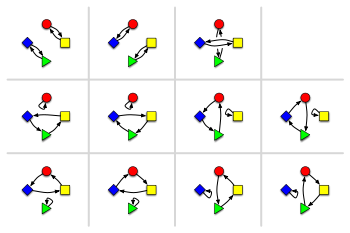
\includegraphics[scale = 0.7]{images/Stirling1.png}
        \caption{Permutations on 4 elements with 2 cycles }
        \label{Fig:StirlingI}
    \end{figure}
\subsection{Stirling numbers of the first kind (${n \brack k}$)} The number of ways of permuting $n$ elements such that the permutations have $k$ cycles is given by the Stirling number of the first kind ${n \brack k}$. Figure \ref{Fig:StirlingI} shows all possible ways of permuting 4 elements with 2 cycles (${4 \brack 2} = 11$). From the definition of ${n \brack k}$, it can clearly be seen that $$n! = \sum_{k=0}^{n} {n \brack k}$$


\Lecture{Jayalal Sarma}{Sept 29, 2020}{10}{Tutte’s Matrix Tree Theorem and counting arborescences}{Raghul}{$\alpha$}{JS}
\section{Introduction}
In this lecture, we will be looking at another application of the Principle of Inclusion-Exclusion(PIE) - Matrix Tree Theorem. We will understand the theorem and then we will cover all the bases required to prove the theorem. The proof of the theorem will be completed in the next lecture.

\section{Kirchoff’s Matrix Tree Theorem} \label{sec:kirchoff's application}
The original theorem for undirected graphs was stated by Kirchoff in the 19th century and the generalised verion for directed graphs was stated by Tutte in the 20th century. This theorem is a classical bridge between combinatorial and algebraic quantities. Let us define few important terms before we jump into the theorems and proofs.\\
\begin{definition}\textbf{Laplacian Matrix for undirected graphs:} 
For any undirected graph $G(V,E)$ with $n$ vertices, let us define a $n$x$n$ matrix $L(G)$ called the \textit{Laplacian matrix} of $G$ as follows.
\[
  L(G)_{ij} = 
  \begin{cases}
    deg(v_i) &\mbox{if }~ i = j\\
    -1 &\mbox{if }~ i \neq j ~\text{and}~(v_i,v_j)\in E\\
    0 &\mbox{otherwise}
  \end{cases}
\]
\end{definition}
\noindent
It can also be noted that for a graph $G(V,E)$ without any self edges (i.e. $\forall i, ~ (v_i,v_i) \notin E$), the Laplacian matrix can also be defined as $L(G) = D - A$ where $D$ is a diagonal matrix with $D_{ii} = ~deg(v_i)$ and $A$ is the adjacency matrix of $G$.
\begin{theorem} Matrix Tree Theorem for undirected graphs by Kirchoff:\\
For any undirected graph $G(V,E)$, the number of different spanning trees rooted at $v_i$ contained in $G$ is given by $det(L_G[i])$ where $L_G[i]$ refers to the matrix obtained by removing the $i^{\text{th}}$ row and the $i^{\text{th}}$ column from $L(G)$ (for any $i \in [n]$).
\end{theorem}
\noindent
Note that the theorem has connected a combinatorial quantity to an algebraic one. It should also be noted that $det(L_G[i])$ is the same for every value of $i$ (since the number of undirected spanning trees does not change with the root $v_i$). The usual proof of this theorem is done using induction on the number of vertices. Instead we will use PIE to prove the generalised version and this theorem will follow as a consequence. Before doing the proof, let us cover few other concepts required for the proof.
\section{Determinant of a Matrix}\label{sec:determinant of a matrix}
From high school mathematics; we all know that for a 2x2 matrix $A$ and a 3x3 matrix $B$, the determinants are given by 
\begin{align*}
  det(A) &= a_{11}a_{22}-a_{12}a_{21}\\
  det(B) &= b_{11}b_{22}b_{33}-b_{11}b_{23}b_{32}-b_{12}b_{21}b_{33}+b_{12}b_{23}b_{31}+b_{13}b_{21}b_{32}-b_{13}b_{22}b_{31}
\end{align*}
It is to be noticed that in the determinant expression of a $n$x$n$ matrix, the subscripts in each term match with one of the $n!$ possible permutations on $[n]$ and there are $n!$ terms in the expression. For example; the first term in the expression for $|A|$ represents the permutation $[1\rightarrow1; ~2\rightarrow2]$ and the other term represents $[1\rightarrow2; ~2\rightarrow1]$. Similarly, the second term in the expression for $|B|$ represents $[1\rightarrow1; ~2\rightarrow3;~3\rightarrow2]$ while the fifth term represents $[1\rightarrow3; ~2\rightarrow1;~3\rightarrow2]$.\\
Thus, each term in determinant expression of a $n$x$n$ matrix represents one of the permutations of $[n]$ and all the permutations are represented exactly once. In other words, given a permutation $\sigma$ on $[n]$, the term $\prod_{i=1}^{n} a_{i\sigma(i)}$ appears exactly once in the expression of the determinant of a $n$x$n$ matrix $A$.\\
Given any permutation $\sigma$ on $[n]$, we can represent it in the point representation as a $n$-tuple as $(\sigma(1),\sigma(2),\sigma(3)\ldots \sigma(n))$. We can define the number of inversions of $\sigma$ ($Inv(\sigma)$) as follows.
$$Inv(\sigma) = |\{(i,j)~|~i<j~\text{and}~\sigma(i)>\sigma(j)\}|$$
For example; for the permutation $\sigma_1 = (1,3,2)$, $Inv(\sigma_1) = 1$ (since (2,3) is the only such $(i,j)$ pair); for $\sigma_2 = (3,1,2)$, $Inv(\sigma_2) = 2$ (since (1,2) and (1,3) are the $(i,j)$ pairs) and for $\sigma_3 = (3,2,1)$, $Inv(\sigma_3) = 3$ (since (1,2), (2,3) and (1,3) are the $(i,j)$ pairs). \\
It can be noticed that the sign of a term representing the permutation $\sigma$ in the determinant expression is given by
$$Sign(\sigma) = (-1)^{Inv(\sigma)}$$
From the inferences done above, one can logically guess the determinant expression for a $n$x$n$ matrix $A$ in terms of
$Sign(\sigma)$ and $\prod_{i=1}^{n} a_{i\sigma(i)}$. However, until proven mathematically, this remains nothing more than a logical guess. So, let us state this as a theorem and prove it.
\begin{theorem}
For any $n \in \N$, the determinant of the $n^{\text{th}}$ order square matrix $A$ is given by
$$det(A) = \sum_{\sigma \in S_n} Sign(\sigma)  \prod_{i=1}^{n} a_{i\sigma(i)}$$
where $S_n$ is the set of all permutations on $[n]$. 
\end{theorem}
\begin{proof}
We know that the determinant of any matrix $A$ follows the following four properties.
\begin{enumerate}
    \item If all the elements in a row of $A$ are 0, then $det(A)=0$
    \item If two rows of $A$ are identical, then $det(A)=0$
    \item If a row of $A$ is a multiple of another row, then $det(A)=0$
    \item Adding the multiple of a row of $A$ to another row, does not change the value of $det(A)$
\end{enumerate}
Though not done as part of the lecture, it can be proven that there is only one expression in terms of $a_{ij}$'s that satisfies all the four properties. Therefore, it is sufficient to prove that the expression given in the theorem satisfies all the four properties stated above to prove the whole theorem. \\
Let us now prove the first property : Let all the elements in row $k$ be 0 i.e. $\forall_{j\in[n]}~ a_{kj} = 0$. It can clearly be seen that each term in the determinant expression stated in the theorem has some $a_{k\sigma(k)}$ in it. So each term will be 0 and hence $det(A)=0$. \\
Proving that the expression stated in the theorem satisfies the other three properties is left as an exercise for the students.
\end{proof}

\section{Applications of PIE} \label{sec:Applications of PIE - lec3}
\subsection{Tutte’s Matrix Tree Theorem} \label{subsec:tutte's application}
 Now, let us continue our journey towards stating and proving Tutte's Matrix Tree Theorem. Firstly, let us define Spanning Arborescences - the directed graphs equivalent for spanning trees and Laplacian matrix for directed graphs.
\begin{definition}\textbf{Spanning Arborescences:} An \textit{Arborescence} is a directed graph in which a vertex $u$ is called the root and for every other vertex $v$ in the graph, there is exactly one directed path from $u$ to $v$. In simpler terms, an arborescence is an directed tree in which all the edges are directed away from the root. A \textit{Spanning Arborescence} $S(V,E)$ of a directed graph $G(V',E')$ is an arborescence such that $V=V'$ and $E\subseteq E'$.
\end{definition}
\noindent\\
\begin{definition}\textbf{Laplacian matrix for directed graphs:} For any directed graph $G(V,E)$ with $n$ vertices, let us define a $n$x$n$ matrix $L(G)$ called the \textit{Laplacian matrix} of $G$ as follows.
\[
  L(G)_{ij} = 
  \begin{cases}
    indeg(v_i) &\mbox{if }~ i = j\\
    -1 &\mbox{if }~ i \neq j ~\text{and}~(v_i,v_j)\in E\\
    0 &\mbox{otherwise}
  \end{cases}
\]
\end{definition}
\begin{theorem} Tutte's Matrix Tree Theorem for directed graphs\\
For any directed graph $G(V,E)$, the number of different spanning arborescences rooted at $v_i$ contained in $G$ is given by $det(L_G[i])$ where $L_G[i]$ refers to the matrix obtained by removing the $i^{\text{th}}$ row and the $i^{\text{th}}$ column from $L(G)$ (for any $i \in [n]$).
\end{theorem}
\noindent
Note that since spanning arborescences are directed, the number of spanning arborecences depend on the chosen root. Hence, unlike the undirected case, $det(L_G[i])$ here depends on the value of $i$. Without loss of generality, we can choose $i = n$ for our proof. Therefore, all we should prove is the number of spanning arborescences rooted at $v_n$ for the directed graph $G$ is given by
\begin{align}
    det(L_G[n]) = \sum_{\sigma \in S_{n-1}}~
    Sign(\sigma)~\prod_{i=1}^{n-1}l_{i\sigma(i)}
    \label{eq:to_prove:Tutte}
\end{align} 
The R.H.S. of the equation is the determinant expression for the $(n-1)$x$(n-1)$ matrix $(L_G[n])$.\\Now let us define another type of directed graphs called Spregs to help with our proof process.\\
\noindent\\
\begin{definition}\textbf{Spregs:} Single prdecessor graphs or \textit{Spregs} with distinguished vertex $v$ of a directed graph $G(V,E)$ is a subgraph $T(V,E')$, $E' \subseteq E$, such that each vertex in $T$ except the vertex $v$ has exactly one predecessor and the vertex $v$ has no predecessors. In other words; in the spreg T, $indeg(v) = 0$ and for every $u \neq v$, $indeg(u)=1$.\\
\end{definition}
\begin{figure}[h]
    \centering
    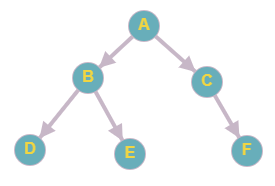
\includegraphics[scale = 0.5]{images/Spreg1.png}
    \caption{Both spreg and arborescence}
    \label{Fig:Spreg1}
\end{figure}
\begin{figure}[h]
    \centering
    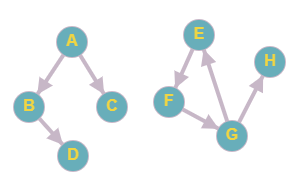
\includegraphics[scale = 0.6]{images/Spreg2.png}
    \caption{Spreg but not arborescence}
    \label{Fig:Spreg2}
\end{figure}
\noindent\\
It is important to distinguish between spregs and spanning arborescences : spregs may contain disconnected components and cycles in them. On the other hand, spanning arborescences are directed spanning trees and hence are single connected components and do not have cycles in them. The directed graph in figure \ref{Fig:Spreg1} is a spreg with distinguished vertex $A$ and an arborescence rooted at $A$. On the other hand, the graph in figure \ref{Fig:Spreg2} is a spreg with distinguished vertex $A$ but not an arborescence. Now let us consider the following lemma and prove it.
\noindent\\
\begin{lemma} If $T(V,E)$ is a spanning arborescence rooted at $v$, then $T$ is a spreg with distinguished vertex $v$.
\end{lemma}
\begin{proof}
Let $T(V,E)$ is a spanning arborescence rooted at $v$. We know from the definition that for every other vertex $u$ in $T$, there is a unique directed path from $v$ to $u$. The underlying undirected graph of $T$ is a tree and does not have any cycles and hence there should not be any cycles (directed/undirected) in $T$.\\
Let us now assume that $indeg(v) \neq 0$. This means that there exists a vertex $u$ in $T$ such that the edge $e = (u,v)\in E$. We know that there is a unique path in $T$ from $v$ to $u$ - let that path be $P$. Now the path $P+e$ is a directed cycle in $T$. A contradiction. Therefore, $indeg(v) = 0$.\\
Let us now assume that for some $u \neq v$ in $T$, $indeg(u) = 0$. This implies that T is not a spanning arborescence.  A contradiction. Therefore, $indeg(u) > 0$. \\
Let us now assume that for some $u \neq v$ in $T$, $indeg(u) \geq 2$. This implies $\exists u_1 \neq u_2$ such that $e_1 = (u_1,u) \in E$ and $e_2 = (u_2,u) \in E$. We know that there exists a unique path $P_1$ from $v$ to $u_1$ and another path $P_2$ from $v$ to $u_2$. Since $u_1 \neq u_2$, $P_1 \neq P_2$. Now, $P_1+e_1$ and $P_2+e_2$ are two distinct paths from $v$ to $u$. A contradiction. Therefore, $indeg(u) = 1$.\\
Therefore,  $indeg(v) = 0$ and for every other vertex $u$, $indeg(u) = 1$. In other words, $T$ is a spreg with distinguished vertex $v$.
\end{proof}
\noindent It is important to note that the converse of the above stated lemma is not true because spregs may contain discconnected components and cycles in them. Now, we will look at another lemma.
\noindent\\
\begin{lemma} If $T(V,E)$ is a spreg with distinguished vertex $v$, then the spreg consists of an arborescence rooted at $v$ and zero or more weakly connected components (the underlying undirected component is connected). Each of these weakly connected components have exactly one directed cycle in them.
\end{lemma}
\begin{proof}
The proof of this lemma is left as an exercise for the students to complete.
\end{proof}
\noindent Thus; (a spreg  with distinguished vertex $v$) = (an arborescence rooted at $v$) + $k$ (weakly connected components with one directed cycle each); where $k \geq 0$. \\
\noindent\\
For proving Tutte's theorem; the idea to count the number of arborescences rooted at $v_n$ is that we would count the number of spregs with distinguished vertex $v_n$ and then remove the number of spregs that are not arborescences - the terms in such a expression would exactly match with that of the R.H.S. of \ref{eq:to_prove:Tutte}.\\
\noindent\\
In the R.H.S. of \ref{eq:to_prove:Tutte}, consider the term for $\sigma =$ identity permutation i.e. $\forall i,~ \sigma(i)=i$. Clearly, $Sign(\sigma)=1$ since $Inv(\sigma)=0$. The term would be $+ \prod_{i=1}^{n-1}l_{ii}$. This is exactly equal to the total number of spregs with distinguished vertex $v_n$ - the reasoning is as follows.\\
Since $v_n$ is the distinguished vertex, ignore all the edges whose end vertex is $v_n$. For every other vertex $u$, choose exactly one of the edges whose end vertex is $u$ ($\prod_{i=1}^{n-1}indeg(v_i)$ ways). Clearly, such a subgraph is a spreg - by definition of spregs. Therefore, the number of distinct spregs is $\prod_{i=1}^{n-1}indeg(v_i) = \prod_{i=1}^{n-1}l_{ii}$ (by the definition of Laplacian matrix). \\
\noindent\\
We have counted all the spregs; now, spregs with cycles have to be removed from the count. This part of the proof involves PIE and will be done in the next lecture.


\Lecture{Jayalal Sarma }{ 2 october, 2020}{More on PIE, PIE -Tuttes-Matrix-Tree-Theorem-Part2}{Shrinidhi Bajpayee}{$\alpha$}{JS}

\section{Introduction}
We finished Tutte's Matrix Tree Theorem in non trivial way.Let's just recall Tutte's Theorem.We have directed graph G(V,E).We have V={v1,v2,....vn}.\\
A $n$x$n$ matrix $L(G)$ called the \textit{Laplacian matrix} of $G$ as follows.
\[
  L(G)_{ij} =
  \begin{cases}
    indeg(v_i) & \mbox{ if } i = j,                                     \\
    $$ $$ -1   & \mbox{ if }~ i \neq j ~\text{and}~(v_i,v_j)\in E$$  $$
    $$ $$ 0    & \mbox{ otherwise (When there is no edge) } $$ $$
  \end{cases}
\]
What theorem says,the number of spanning arborescences rooted at some vertex n is given by exactly equal to $det(L_G[i])$ Here i=n.\\
Quickly Recap Definition of Spanning arborescences :An \textit{Arborescence} is a directed graph in which a vertex $u$ is called the root and for every other vertex $v$ in the graph, there is exactly one directed path from $u$ to $v$. In simpler terms, an arborescence is an directed tree in which all the edges are directed away from the root. A \textit{Spanning Arborescence} $S(V,E)$ of a directed graph $G(V',E')$ is an arborescence such that $V=V'$ and $E\subseteq E'$.\\
One condition is that there is a directed path from V to every vertex in G within E'.\\
Second condition is underlying undirected graph should be a tree. \\ \\
Let's just take away of Last Lecture .\\
One take away is as following:\\
\begin{align}
  det(L_G[n]) = \sum_{\sigma \in S_{n-1}}~
  Sign(\sigma)~\prod_{i=1}^{n-1}L_{i\sigma(i)}
  \label{eq:to_prove:Tutte}
\end{align} \\
$S_(n-1)$ is notation for permutation of $n-1$.\\
This is expression of determinant that we have seen in last lecture.\\
So we want to show it is equal to spanning arborescence we introduce concept called Spreg.So what is Spreg $?$.\\
We quickly define Spreg.\\
\begin{definition}\textbf{Spregs:} Single prdecessor graphs or \textit{Spregs} with distinguished vertex $v$ of a directed graph $G(V,E)$ is a subgraph $T(V,E')$, $E' \subseteq E$, such that each vertex in $T$ except the vertex $v$ has exactly one predecessor and the vertex $v$ has no predecessors. In other words; in the spreg T, $indeg(v) = 0$ and for every $u \neq v$, $indeg(u)=1$.\\
\end{definition}\\
Every vertex other than distinguished vertex must be indegree 1.Subgraph of G is called Spregs.So there are several spregs are possible similar to several spanning arborescence possible.\\
We want to count spanning arborescence using spregs.That will be very nice combinatorial interpretation of this topic,that is plan.\\

1. We want to count the number of spanning arborescence rooted at Vn.\\ \\
2.We want to count the number of spregs distinguished vertex Vn.\\
We associated with last lecture that every spanning arborescence corresponds to spregs .It turns out there are more spregs.There is some structure,Spregs looks like are of the form arborescence $+$ weekly connected component 1 $+$ weekly connected component 2......\\
V can not be part of cycle.V can be vertex in component.Weekly connecetd component has exactly 1 cycle.\\
So what we want to count spregs in inner circle with distinguished vertex Vn.Ok so already know what we have to count.Basic strategy is as follows:\\
Strategy is that count the number of spregs with distinguished vertex Vn which does not have any cycle.So this is what we want to count.We want to use Inclusion Exclusion.In fact we will not only count through Inclusion exclusion but we will go through each term of the determinant expression corresponds to our counting terms.\\
Let's demonstrate by writing down Inclusion exclusion.\\
In order to define Inclusion Exclusion formulation we need to define the \\ \\
1.Universe (Called as X).\\
2.Component $A_i$.\\
To define that Let's consider,notice that we want to count spregs without any cycle.\\
We need to be set of all spregs with distinguished vertex Vn.\\
Let $C_1$,$c_2$,$C_3$,.....$C_n$ be the set of cycles in graph G.We looking at simple cycle.\\
$A_i$ define as spregs which contain the cycle $C_1$.The number of spregs which does not contain any cycle.This what we want to count.So,\\

$|X|$ $-$ $|\bigcup_{i=1}^{n} A_i|$\\
It is same as,
&=$$|X| - \sum_{I \subseteq [n] , I \neq \emptyset} (-1)^{|I|+1}|\bigcap_{i \in I} A_i|$$\\
So already applied Inclusion Exclusion,Now write it as
&=$$ |X| + \sum_{I \subseteq [n] , I \neq \emptyset} (-1)^{|I|+1}|\bigcap_{i \in I} A_i| $$\\
So basically we need to count this.We can say that each term in these expression are exactly same as term used in determinant expression.As number of Spregs are equal to number of spanning arborescence,hence theorem is called.This is strategy.Hence each term is associated with terms of determinant theorem.\\
\textbf{Observation:}Let's consider C1,C2 be two cycles.\\
What can say about $$ A1 \bigcap A2 = \emptyset iff C1
  \bigcap C2 \neq \emptyset.$$\\
Every spregs looks like arborescence + uniquely weekly connected component 1 +uniquely weekly connected component 2.\\
$$ If C1 \bigcap C2 \neq \emptyset then |A1 \bigcap A2| =0.$$\\
Using the observation,\\
The number of spregs with distinguished vertex Vn which is acyclic is nothing but \\
&= $$ |X| + \sum_{I \subseteq [n] ,I \neq \emptyset ,for J,K \belongs I, J \neq K, cj \bigcap ck =\emptyset}       (-1)^{|I|+1}|\bigcap_{i \in I} A_i| $$\\

\textbf{Recall:} We counted |X| =Total number of spregs\\
$$det(L_G[n]) = \sum_{\sigma \in S_n} Sign(\sigma)  \prod_{i=1}^{n} a_{i\sigma(i)}$$\\
This is determinant expression.\\
&= term   corresponds   to   $$ \sigma=id $$\\
&= $$\prod_{i=1}^{n-1} (L_i) = \prod_{i=1}^{n-1} deg_in(L_i) $$\\
Now we count the singleton sized I.\\
Spregs that contain exactly one cycle.\\
Fix,I={1},We are counting spregs which contain only C1.\\
Let  CI be (Vi1,Vi2,Vi3,....Vin)\\
$$\sigma(i1)=i2$$\\
$$\sigma(i2)=i3$$\\
$$\sigma(ik-1)=ik$$\\
$$\sigma(ik)=iI$$\\
$$\sigma \in S_n-1$$\\
$$\forall other  i \in {1...n} $$\\
$$ \sigma(i)=i $$\\
This is permutation which contain one cycle.\\
Now we just able to do following\\
\textbf{Claim:} Term in the determinant expression for\\
$$LG[n] corresponds to \sigma=number of spregs which contain C1$$ \\
Right now we are talking about one circle.\\
Let's see proof of this.\\
Proof of this is very natural.
$$sign(\sigma)\prod_{i=1}^{n-1} L_i,\sigma(i   $$\\
sign of permutation is exactly equal to
$(-1)^{(l-1)} $.Here length is l.\\
Second term is \\
$$ (-1)^{(l-1)} (\prod_i,|\sigma(i)|=i L_i,i)(\prod_i,|\sigma(i)| \neq i L_i,\sigma(i)) $$\\
$$ L_i,\sigma(i) =-1,if V_i,V_\sigma(i) is edge in graph \in E\\ ootherwise  $$\\
If corresponding edge is present then this term is non zero otherwise zero.\\
$$ (-1)^{(l-1)}(\prod_i,|\sigma(i)| deg_in(v_i))*(-1)^{l} $$\\
$$&= (-1)^{(2l-1)} |number of spregs which contain C1|  $$\\
$$&= -|number of spregs which contain C1 | $$\\
Proposition for $$ \sigma \in S_n-1 comsisting of single cycle.   $$\\
$$ \sigma =(i1,i2,.....il)   $$\\
Associate$ C\sigma $ as a cycle corresponds to vertex sequence (Vi1,Vi2,Vi3.....Vil,Vii)\\
Then the term in the determinant corresponds to $\sigma$ satisfies following.\\
$$sgn(\sigma)(\prod_{i=1}^{n-1}L_i,\sigma(i))$$

$$ &= -(\prod_{i,\sigma(i)=i}deg_in(v_i))C_\sigma \subseteq G(V,E) $$\\
$$ 0 if C\sigma \nsubseteq G(V,E) $$ \\
$$-1  if C\sigma \subseteq G(V,E) if \forall i \sigma(i) \neq i     $$\\


\textbf{Corollary:}$$For \sigma,C\sigma as above $$\\
$$ |\prod_{i=1}^{n-1}L_i,\sigma(i)|=number of spregs which contain C_\sigma   $$\\
Now this is case for single cycle.\\Now we will generalise case for multiple cycle.\\
So it is very natural.\\
\textbf{Question:}Suppose $\sigma$ \in $S_n-1$ is the product of K>0 disjoint cycle.\\
$$\sigma=(i11,i12,i13.....iil) (i21,i22,i23....(ikl,ik2,ik3...ikl)    $$
K is number of cycles.\\
So now we are associate \\
$$ C_\sigma = \cup  {j=1}^{k}C_j  where C_j is ()V_ij1....V_ijLj.....VijI)$$\\
Then the term  corresponds to $\sigma$ in $det(L_G[n])$\\
$$sgn(\sigma) = (-1)^{K} \prod_{i|\sigma(i)|}deg_in(V_i) if C_\sigma \subseteq G   $$\\
$$ o if C\sigma \nsubseteq G $$

\textbf{Corollary:}If we look at\\
$$|\prod_{i=1}^{n}L_i,\sigma(i)|=number of spregs which contain C_\sigma = \bigcup_{j=1}^{k}C_j   $$\\
$$ det(L_G[n]) =\sum_{\sigma \in S_n-1}sig(\sigma) \prod_{i=1}^{n} L_i\sigma      $$\\
This is how determinant expression looks like.\\
Number of spanning arborescence rooted at Vn  as distinguished vertex and not containing cycle.\\
$$&=|X| + \sum_{I \subseteq [n] ,I \neq \emptyset, cj \bigcap ck=\emptyset ,j,k \in I}(-1)^I    $$\\
This is strategy.
This lecture is combinatorial application of PIE.

\newpage
WEEK 4 LECTURE 2\\
Algorithmic Application of PIE
\section{Introduction} We talk about counting problem.Its about given a $n*n$ bipartite graph,We want to count the number of perfect matching in it?\\
subset of edges such that every vertex has exactly one edge incident on it from the
subset.\\
Bipartite adjacency matrix is different from adjacency matrix.\\ \\
\textbf{Trivial Algorithm:}Run through all n sized subsets of E.\\
$${n^{2} \choose n } \sim {n^{2} \choose n}^{n}    \sim n^{n} \sim 2^{nlogn}$$\\

$$ {n \choose k}^{k} \leq {n \choose k} \leq {n_e \choose k}^{k} $$\\
e=natural log base \\
\section{Decision Problem:}
\textbf{Binpacking Problem:}
Given a positive integer (bin capacity B),positive integer k\\
We have n item with weight S1,S2,S3.....,Sn\\
partition the items into u1,u2,u3.....,uk\\
Capacity is such that sum of weights of items in each ui is almost B.\\
This is binpacking problem.\\
It is NP-problem.\\
By PIE Time complexity is $O(nB2^{n})$\\
n=number of items\\
B=capacity\\
Now we will reformulate PIE.\\

Given a collection of N combinatorial objects \\
Let p(1),p(2),p(3)...p(n) be properties.\\
$p_i$ is essential function \\
$$ N \to {0,1}   $$\\
It is possible that some object doesn't have properties of that.\\
$$N_i \to Number of objects among N with property P(i).$$\\
$$ {i_1,i_2,....i_r} \subseteq {1,2,3,...N} $$\\
$$N_i_1,i_2,i_3....i_r = Number of objects with properties p(i_1) p(i_2)....p(i_r) $$\\
N(0)=Number of objects not having any of the property.\\
$$ N(0)=N-\sum_{i=1}^{n} N_i_1 +\sum_{i_1<i_2}N_i_1,i_2 -\sum_{i_1 < i_2 <i_3}.......(-1)^{j} \sum_{i_1<i_2<...i_j}N_i_1,i_2...i_j (-1)^{x}N_1...r   $$\\
Restatement (Complementary term)(For the discussion)\\
$$N \to Number of objects.$$\\
$$Q(1),Q(2),....Q(n) $$be properties that some of these objects have.\\
$$W \subseteq {1,2,....n}  $$\\
Let N(W) be the number of objects having none of the properties Q(i).\\
$$i \in W   $$\\
Now what we want to count the other set.\\
$$X \to number of objects which has all the properties.$$\\
$$X = \sum_{W \subseteq [n]}(-1)^{|W|} N(W)   $$\\
\textbf{Pf:}$Define P(i) iff \neg Q(i)$\\
Now the above restatement is applicable.\\
Given a bipartite graph $G(u,v,E)\\
  |u|=|v|=n $\\
count the number of perfect matching.\\
\textbf{I/p:}Bipartite adjacency matrix.\\
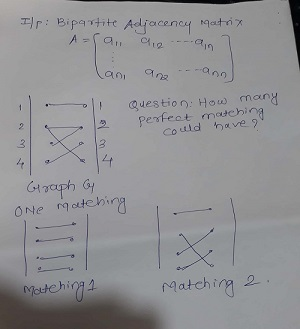
\includegraphics{graph.jpg}\\ \\
There are 2 perfect matching is in these graph.\\
Matching 1: There is bijection.\\
There are 4!=24 permutation.But matching 1 and matching 2 are two permutation for perfect matching.\\
How's the algebric way of writing itself.\\
Let's write $\sigma \in S_n$ \\
Consider,\\
$$ \prod_{i=1}{n} a_i \sigma(i)$$\\
When $a_i \sigma_i$ is non zero value.
When $i\sigma _i$ is true.\\
$$\prod a_ii = a11 .a22 .a33. a44$$\\
$$ &=1 $$\\
What will be product of \\
$$\prod_{i=1}{n} a_i \sigma(i) $$\\
$$ &=a12. a21.a33.a44  $$\\
$$ &=0  $$\\
If corresponding edge is there in graph then value will be 1 otherwise 0.\\
a12=0 since no edge from 1 to 2.\\
Let's write,\\
Permanant of A=\\
$$ \sum_{\sigma \in S_n}  = Number of perfect matching in the graph.$$\\
Given a matrix A,\\
Its two types are:\\
!)permutataion (A) that is per(A): It is number of perfect matching in graph.\\
2)Determinant (A) that is det(A)\\
\\
\textbf{Problem:}Given a matrix A o/p the value of per(A)\\
\textbf{Trivial Algorithm:}Run over all $\sigma \in S_n$ compute the product \\
$$\prod_{i=1}{n}a_i \sigma(i)$$ and add.\\
$$O(n!) \sim O(n ^{n}) \sim 2^{nlogn} $$\\
\textbf{Lemma:}A is bipartite adjacency matrix of a bipartite graph G\\
$$Per(A) = \sum_{W \in {1...n}}(-1)^{|W|} \prod_{i=1}^{n}(\sum_{j \notin W}a_ij)$$\\
Applying Lemma,\\
$2^{n}$ W's and n^{2}=remaining Computation\\
2^{n}n^{2} time algorithm.\\
\textbf{PF:}To apply complementary form PIE.\\
Define N objects: M \in N\\
M \subseteq E such that for  every \\
$\forall i \in {1...n}$ the vertex $X_i$ is the endpoint of some vertex in M.\\
$\forall j \in [n] Q(j)$: Vertex $Y_j$ is the endpoint of some vertex in M.\\
We want to count number of objects from underlined part which satisfies Q(1) .....Q(n)\\
The number of perfect matching=per(A)=number of objects which satisfies all of Q(1) Q(2)....Q(n)\\
Q(1) says first one is matched.\\
Q(2) says second one is matched.\\
Like this etc etc.\\
When all vertex are matched from both side.\\
$$ &= \sum_{W \in {1...n}}(-1)^{|W|}$$\\
N(W)=Number of objects which satisfies none of property in W.\\
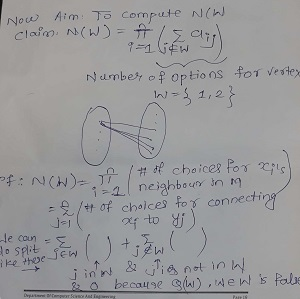
\includegraphics{img.jpg}\\ \\
Per(A)=Number of perfect matching.\\
$$ &=\sum_{W \subseteq {1...n}}(-1)^{|W|}(\prod_{i=1}^{n}(\sum_{j \in w}aij)) $$\\
This completes the proof of the Lemma.\\
This lemma gives O(2^{n}n^{2}) algorithm for computing number of perfect matching in a given bipartite graph.\\
NP complete=Decision Problem.\\
#p(partly)complete=counting complexity.\\
\textbf{Quickly Recap:}\\
\textbf{Binpacking problem:}\\
$Bin capacity B,We have number of bins K,We have n items S1....Sn are sizes.$\\
$Question is Can we partition items to u1....uk[n]such that$\\\
$$\forall_{$i\leq j \leq k}j\sum_{i \in u}Si \leq B$   $$\\
  We want to count this.\\
  \textbf{Algorithm:}\\
  \textbf{Trivial Algorithm:}Run through partition.\\
$$ n \choose k$$\\
  O(nB2^{n}) time space.\\
  A partition of [n] into u1....uk is said to be feasible if the sum of the sizes of item $\leq$ B in uj.\\
  \textbf{Relax:}Items can appear more than once.\\
  \textbf{observation:}A feasible solution with relaxation will remain feasible without relaxation.\\
  \textbf{Relaxed Solution:}ordered set of K lists of items from {1...n}.\\
  1.Each of the elements in {1...n}appears atleast in one list.\\
  2.For each list a1,a2....ap
$$\sum_{h=1}{p}S_ak \leq B $$\\
  To apply PIE,we need to define objects Q1....\\
  \textbf{Objects:}Ordered sets of K list of elements from {1...n} such that for each list (a1...ap) $$\sum_{h=1}{p}S_an \leq B $$\\
  Q(1):=The ordered list of k lists contain 1 in atleast one list in it.\\
  .\\
  .\\
  .\\
  Q(W):=W  is contained in atleast one of the lists in the ordered set of list.\\
  .\\
  .\\
  .\\
  Q(n)\\
  X=Set of objects which satisfy all of the properties Q(1)....Q(n)\\
$$X=\sum_{w \subseteq [n]}(-1)^{|w|} N(W) $$\\
  \textbf{Aim:}To compute N(W)\\
  A(W):=Number of list a1....ap of elements list in W.\\
$$ \sum_{h=1}{p}S(an) \leq B $$\\
$$N(W)=(A(W))^{k}  $$\\
  \textbf{Aim:}Compute A(W)\\
  $P_w(j)$ =number of list a1....ap of which element not in w such that
$$\sum_{h=1}{p}S(ak)=j  $$\\
$$A(w)=\sum_{j=0}{B}P_w(j)$$\\
$$P_w(j)=\sum_{i \notin w}P_W(j-s(w)) $$\\
$$ p_W(j)=0, j<0 $$\\
$$P_w(0)=1 $$\\
Time taken is O(nB2^{n})


% Lecture 3


\Lecture{Jayalal Sarma}{Oct 10, 2020}{13}{From Principle of Inclusion-Exclusions to Mobius Inversion}{Sandip Saha}{$\alpha$}{JS}

% \section{Introduction}
The journey so far has been that we have started with pigeon hole principle and its applications then we used double counting and bijections to establish different identities then we moved to PIE and its different applications.
% Then we came to Principle of Inclusion-Exclusion(PIE) as a consequence of a bijection argument. 
In this lecture, we will look at a more generalized version of PIE and move gradually towards the Mobius Inversion.

\subsection{PIE Revisited}
Previously we have used PIE to compute $\left| \bigcup^n _{i=n} A_i \right|$ as follows,
\[ \left| \bigcup^n _{i=n} A_i \right|=\sum_{\emptyset \neq I \subseteq [n]} (-1)^{|I|+1}\left|\bigcap_{i\in I} A_i\right|\]
Now, we are interested to compute $\left|\bigcap_{i=1}^n  \overline{A_i}\right|$, which can be rewritten as,
\begin{align}
  \left|\bigcap_{i=1}^n  \overline{A_i}\right| & = \left|
  \overline{\bigcup_{i=1}^n  A_i}
  \right| \nonumber \tag{using De-morgan's law}                                                                                                                    \\
                                               & = \left| X \right| - \left| \bigcup^n _{i=n} A_i \right| \nonumber                                                \\
                                               & = \left| X \right| -\sum_{\emptyset \neq I \subseteq [n]} (-1)^{|I|+1}\left|\bigcap_{i\in I} A_i\right| \nonumber \\
                                               & = \sum_{ I \subseteq [n]} (-1)^{|I|}\left|\bigcap_{i\in I} A_i\right|
\end{align}

Note that $\bigcap_{i\in \emptyset} A_i =X$. This thing can also be stated in the following way.

\begin{theorem}
  Let $X$ be a finite set and $P_1,\dots, P_m$ properties. Further define for $S \subseteq [m]$ the set $N(S) = \{x\in X \mid \forall i \in S: x \text{ has property } P_i\}$  then, number of elements in $X$ satisfying none of the properties $P_1,\dots, P_m$ is given by,
  $$ \sum_{S \subseteq [m]} (-1)^{|S|} \left| N(S) \right|$$
\end{theorem}

\subsection{Stronger version of PIE}
The Inclusion-Exclusion Principle has a stronger version which is as follows.

\begin{theorem}[Stronger PIE]
  \label{stronger PIE}
  Let $f,g:2^{[n]}\longrightarrow \mathbb{R}$ are functions assigning real numbers to subsets of $[n]$ with the property that for any $A\subseteq [n]$

  \[ g(A)=\sum_{S\subseteq A} f(S)\]

  Then,
  \[ f(A) = \sum_{S \subseteq A} (-1)^{|A|-|S|}g(S)\]

\end{theorem}


\begin{proof}
  Let $f$ and $g$ are functions from the powerset of $[n]$ to real numbers and for all $A \subseteq [n]$
  \[g(A)=\sum_{S\subseteq A}f(S)\]

  \begin{align}
    \sum _{s\subseteq A}( -1)^{|A|-|S|} g( S) & =\sum _{s\subseteq A}( -1)^{|A|-|S|}\left(\sum _{T\subseteq A} f( T)\right) \nonumber \\
                                              & =\sum _{T\subseteq A} C_{T} f( T)
  \end{align}
  Where $C_T$ is appropriate signed number. Our aim is now to find $C_T$ for different $T$

  \begin{description}
    \item{\textbf{Case 1: }($T=A$)} $C_T=1$, since $f(A)$ is only encountered for $T=S=A$.

    \item{\textbf{Case 2: }($T \neq A$)} choosing a set between $T$ and $A$ is equivalent of choosing a set from $A\setminus T$
          \[C_T=\sum _{T \subseteq S\subseteq A}( -1)^{|A|-|S|}=\sum^k_{i=0}(-1)^{k-1} {k \choose i} =0 \]
  \end{description}
  This proves the claim.
  \[\boxed{\therefore f(A) =  \sum_{S \subseteq A} (-1)^{|A|-|S|}g(S)}\]
\end{proof}

\textbf{Why it is strong version?} it implies PIE.
Assume the strong version, we can derive PIE.
\begin{proof}
  Properties $P_1,\dots, P_m$ of elements of $X$ . $X_1,\dots, X_m$ are the subsets of $X$ satisfying the respective property i.e. $X_i=\{ x\in X \mid x \text{ satisfy } P_i\}$.
  then for $S \subseteq [m]$  we define $f(S)$ to be the number of elements in $X$ having all properties $P_i$ such that $i \notin S$ and none of the properties $P_j$ such that $ j \in S$ i.e.
  \[ f(S) = \left| \bigcap_{i\in [m] \setminus S} X_i \setminus \bigcup_{i\in S} X_i \right| \]
  We are interested in counting the number of elements in $X$ which does not satisfy any property in $P_1,\dots, P_m$ i.e. $f([m])$. We define,

  \begin{align*}
    g(A) & = \sum_{S\subseteq A} f(S)                         \\
         & = \left| \bigcap_{i \in [m] \setminus A}X_i\right| \\
         & = N([m]\setminus A)
  \end{align*}
  $g(A)$ counts $x\in X$ if the property that $x$ does not satisfy forms a subset of $A$. By \ref{stronger PIE}
  \begin{align*}
    f([m]) & = \sum_{S\subseteq [m]}(-1)^{m-|S|} g(S) \\
           & = \sum_{\substack{
    S'\subseteq [m]\setminus S                        \\
        S\subseteq [m]}}
    (-1)^{|S'|} N(S')                                 \\
           & = \sum_{S \subseteq [m]} (-1)^{|S|} N(S)
  \end{align*}
  This concludes the proof.
\end{proof}




\Lecture{Jayalal Sarma}{Oct 5, 2020}{14}{Mobius Inversion and applications}{K Sampreeth Prem}{$\alpha$}{JS}

\section{Introduction}
The focus on this lecture will be if we have two funtions $f$ and $g$ such that g can be expressed as a function of $f$ by a peculiar relation then how can we express $f$ in terms of $g$. We have already seen one such inversion during the discussion of stronger version of PIE where we have two fuctions mapping from sets to numbers. In this lecture we will look at a different setup where we have two functions $f:\{\mathbb{N} \} \to \{\mathbb{N}\}$ and $g:\{\mathbb{N} \} \to \{\mathbb{N} \}$ and if $g$ can be expressed in a peculiar way w.r.t $f$ then we want to invert to express $f$ in terms of $g$.This is called \textbf{Möbius Inversion}.
Before we formally state the theorem and prove it, we will look at two functions namely Euler's function and Möbius function and derive some of their properties.We will then establish a relation between these two functions to prove the Möbius Inversion and then look at an application of the theorem. 

\section{Euler's Function} \label{sec:Euler's Function}
Euler's function, also known as phi-function $\Phi(n)$, counts the number of integers between 1 and n inclusive, which are coprime to n. 
$$
\Phi(n) = |\{k \in \mathbb{N} | 1\leq k \leq n, gcd(n,k)=1\}| \label{fun:euler's}
$$ 
We have already derived the formula for $\Phi(n)$ in \ref{subsec:euler's function application} which is 
\begin{align}
\Phi(n) = n\prod_{i=1}^{k}(1-\frac{1}{p_i}) \textrm{ ~~~where~~  $n = \prod_{i=1}^{k}(p_i)^{a_i} $}\label{for:Euler's formula} 
\end{align}
\subsection{Properties of $\Phi(n)$} \label{subsec:Properties of Euler function}

\begin{property} 
If $gcd(n1,n2)=1 \implies \Phi(n_1)\Phi(n_2) = \Phi(n_1n_2) $  
\end{property} 

\begin{proof}
We have derived this in \ref{subsec:euler's function application}
\end{proof}
                
\begin{property}
$ \sum_{d|n}^{} \Phi(d) = n $
\end{property}

\begin{proof}
Fix $d$ as a divisor of $n$. Consider the following sets $ A = \{x\in\{1,2,..n\} | gcd(x,n)=d\}$ and $B = \{y\in [\frac{n}{d}] | gcd(y,\frac{n}{d})=1\}$. Now we will establish a bijection between these two sets. The cardinality of the second set is $\Phi(\frac{n}{d})$ (by definition of $\Phi$) but instead of counting explicitly we will establish a bijection between A and B. Consider the mapping $x \mapsto \frac{x}{d}$ ,this mapping is well defined because $gcd(x,n) = d$ so $d|x$ and $\frac{x}{d}$ is an integer whose value is at most $\frac{n}{d}$ so it is in the range of B.The mapping is injective because division is injective. Now take any element from $1$ to $\frac{n}{d}$, multiply it with $d$ then we will get a number $p$ such that $gcd(p,n) = d$ because $d$ is the divisor of both $n$ and $p$. So the mapping is also surjective and hence a bijection. 
Observe that the property can be rewritten as, 
$$
\sum_{k = \frac{n}{d}}\Phi(\frac{n}{k})
$$ 
From the bijection established,$$
\sum_{d}|\{x\in\{1,2,..n\}|gcd(x,n)=d\}| = \sum_{k}\Phi(\frac{n}{k})
$$
Notice that the summation on L.H.S will be equal to $n$ that's because every number $l \in [1,n]$ will be counted exactly once in the summation when the variable of summation $d=gcd(x,n)$.\\
So, 
\begin{align*}
n =  \sum_{k}\Phi(\frac{n}{k})\\
\sum_{k}\Phi(\frac{n}{k}) = n
\end{align*}
Hence, the proof.
\end{proof} 

\section{Möbius Function} \label{sec:Möbius Function}
For any positive integer $n$, Möbius Function $\mu(n)$ is defined as, 
53
 
	\[
	\mu(n) = \begin{cases} 
	+1 , & ~if~ ~n~ ~is~ ~a~ ~\href{https://en.wikipedia.org/wiki/Square-free_integer}{square-free} ~positive~ ~integer~ ~with~ ~an~ ~even~ ~number~ ~of~ ~prime~ ~factors~~\\
 	-1 , & ~if~ ~n~ ~is~ ~a~ ~square-free~ ~positive~ ~integer~ ~with~ ~an~ ~odd~ ~number~ ~of~ ~prime~ ~factors~~\\
	0 , & otherwise
	\end{cases}
	\]
\noindent
For example,$15=3*5$ has even number of prime factors which are square-free, hence $\mu(15)=1$. Similarly, $30=2*3*5$ and $20={2^2}*5$ has $\mu$ values equal to $-1$ and $0$. \\
Now, consider the factors of $30$ and their $\mu$ values
\begin{center}
\begin{tabular}{c c c c c c c c c }
 Factors & 30 & 15 & 10 & 6 & 5 & 3 & 2 & 1 \\ 
 $\mu$ & -1 & 1 & 1 & 1 & -1 & -1 & -1 & 1 \\  
\end{tabular}
\end{center}
\noindent
We Observe the sum of $\mu$ values of the factors of $30$ are equal to $0$. This isn't a coincidence and we will formally define this property and prove it.\\

\begin{property} \label{prp:2}
$\sum_{d|n}\mu(d) = \begin{cases} \label{subsec: Properties of Möbius Function }
	1 , & ~if~ n=1\\
	0 , & otherwise
	\end{cases}
	$
\end{property}

\begin{proof}

$$\mu(1) = 1 ~~(~by~ ~definition~)$$
Take $n= \prod_{i=1}^{k}(p_i)^{a_i}$, we will consider only those factors of $n$ whose prime factors have multiplicity $1$ other factors of $n$ which have prime factors multiplicity greater than 1 have $\mu$ value $0$ and does not contribute to the sum.     
\begin{align}
\sum_{d|n}\mu(d) &= \sum_{d|p_1p_2...p_k}\mu(d) \label{pf:pt1} \\
&= \sum_{I\subseteq[k]}{(-1)}^I \label{pf:pt2} \\ 
&= \sum_{i=0}^{k} {k \choose i}{(-1)}^i\nonumber\\
&= 0 \nonumber
\end{align}
Notice that in $\ref{pf:pt1}$ the $\mu$ value depends only on whether we are picking odd number of primes or an even number and not on actual primes themselves so we could rewrite the summation to
$\ref{pf:pt2}$.
\end{proof}
\noindent
Now, we will see a corollary of the above propery that connects the two functions $\mu$ and $\Phi$. \\ 
\begin{corollary} \label{subsec:relation between euler function and mobius function}
$\frac{\Phi(n)}{n} = \sum_{d|n}\frac{\mu(d)}{d} $
\begin{proof}
From \ref{subsec:euler's function application}
\begin{align}
    \Phi(n) &= n\prod_{i=1}^{k}(1-\frac{1}{p_i}) \label{cor:pt1}\\
    &= n\sum_{I \subseteq [k]} (-1)^{|I|}\frac{1}{(\prod_{i \in I}p_i)}\label{cor:pt2}\\
    &= n\sum_{d|p_1...p_k}\frac{\mu(d)}{d} \label{cor:pt3} \\
    &= n\sum_{d|n}\frac{\mu(d)}{d} \label{cor:pt4}
\end{align}
In step \ref{cor:pt2}, $I\subseteq[k]$ can be thought of as those prime indices that are picked which contribute to $d$ so the ${(\prod_{i \in I}p_i)}$ becomes equal to $d$  and the numerator $(-1)^{|I|}$ is exactly $\mu(d)$. The generalisation of step \ref{cor:pt3} to \ref{cor:pt4} is done following the observation that if $d|n$ but $d\nmid\prod p_1..p_k$  then $d$ must have a prime factor whose multiplicity is greater than 1. Therefore, $\mu(d)$ becomes $0$ for such $d$'s.
\end{proof}
\end{corollary}

\section{Möbius Inversion} \label{sec:Möbius Inversion}
$f,g:\mathbb{N} \to \mathbb{R} ~satisfying,$ $\forall n ~g(n) = \sum_{d|n} f(d)  ~~then,$  
$$\forall n ~f(n) = \sum_{d|n} \mu(d)d(\frac{n}{d})$$

\begin{proof}
Consider,
\begin{align}
    \sum_{d|n}\mu(d)g(\frac{n}{d}) &= \sum_{k=\frac{n}{d}}\mu(\frac{n}{d})g(d)  \label{pf:pt1}\\
    &= \sum_{d|n}\mu(\frac{n}{d})g(d) \label{pf:pt2} \\
    &=\sum_{d|n}\mu(\frac{n}{d})(\sum_{d'|d}f(d')\label{pf:pt5} \\
    &=\sum_{d'|n}C_{d'}f(d')  \label{pf:pt3}\\
    &=f(n) \label{pf:pt4}
\end{align}
At \ref{pf:pt3} $C_{d'}$ represents the constant that tells us how many times $f(d')$ is going to appear in the summation. Note that, if $d|n$ then $(\frac{n}{d})|n$ so using a change of variable we were able to reach \ref{pf:pt2} from \ref{pf:pt2}. \\
Now, we have two tasks, first calculate the value of $C_{d'}$ and next to show the summation value of \ref{pf:pt3} is $f(n)$.\\
\item {\textbf{Plan:} Evaluate $(C_{d'})$ for differnet $d'$}
\item \underline{\textbf{Case1:} }\text{~~If $d'=n$ then, $f(n)$ occurs only once in the summation \ref{pf:pt5}}. So, $C_n=1.$ \\

\item \underline{\textbf{Case2:}} $~~d'<n ~~and~~ d'|n.$
\begin{align} 
    C_{d'} &= \sum_{d'|d|n} \mu(\frac{n}{d}) &\label{cs2:p1}\\
    &= \sum_{d|n}\mu(\frac{n}{d}) &\label{cs2:p2}\\
    &= \sum_{d|n}\mu(d) &\label{cs2:p3}\\
    &= 0 \nonumber
\end{align}
In step  $d \neq 1$ so by Property 14.3.1 (\ref{prp:2}) we get the value 0.
Observe that in step \ref{cs2:p1} the summation value doesn't depend on $d'$ so by change of variable we reach step \ref{cs2:p2}.Similarly, we reached step \ref{cs2:p3}  from \ref{cs2:p2} using change of variable that we have seen earlier.\\
Since we have calculated the value of $C_{d'}$ for different $d'$s  we will now show the value of summation in \ref{pf:pt3} is $f(n)$.
\begin{align}
\sum_{d'|n}C_{d'}f(d') &= C_nf(n)~~+~~\sum_{(d'~<~n)|n}C_{d'}f(d')\nonumber\\
&= 1*f(n) + 0 \nonumber\\
&= f(n) \nonumber
\end{align}
Hence, proved. 
\end{proof}
\subsection{Application of Möbius Inversion} \label{Application of Möbius Inversion}
\textbf{Problem Statement:} Count the number of circular sequences/strings of $0$'s and $1$'s of length $n$.\\
\textbf{Solution:} We know that there are $2^n$ possible strings of $0$'s and $1$'s but some of them are clockwise rotations of each other and we consider them equal.So the circular sequences which are clockwise rotations of one another are equivalent. \\
Consider the following example of circular sequences of $0$'s and $1$'s of length 9. In order to represent a circular string in a normal form we fix a starting point and iterate it until it's length.    \\
A = 001011010\\
B = 110100010\\
C = 100100100\\
By our definition of equivalence $A \equiv B \not\equiv C$. \\
Observe that sequence C is periodic, it has a repeating subsequence 100 whereas sequences A and B do not contain any such repeating sub sequence.We call them aperiodic. In general a sequence is said to be aperiodic if it cannot be written as several times of a shorter sequence. \\
For every circular sequence there is a unique aperiodic circular sequence that we can associate with.\\
Instead of proving this claim we will write it as an example \\
For $n=6$,\\
$
000000  \Rightarrow  0 \\
001001  \Rightarrow 001 \\
111111  \Rightarrow  1 \\
010010  \Rightarrow 010 \\
001001  \Rightarrow 001 \\
$
Observe that the last two examples are equivalent and their circular subsequences are also equivalent. So their is an unique association (bijection) of circular sequences and their circular subsequences. \\
Another obvious observation is that the length of the circular subsequence must divide the original sequence. \\
Let, 
\begin{align}
M(d) ~=~ ~no.~ ~of~ ~periodic~ ~circular~ ~sequences~ ~of~ ~length~ ~d~ \nonumber
\end{align}  
Denote, $N_n$ as the number of circular sequences of length n, then \\ 
\begin{equation} \label{eq:circular seq}
    N_n = \sum_{d|n}M(d) 
\end{equation}
Since we don't know the values of $d$ we are summing up over all values of $d$ that divides $n$. \\
Now we need to compute $M(d)$ as a function of $d$.
\textbf{Aim:} Compute $M(d)$ as a function of $d$.
\textbf{Solution:} Consider,the query how many aperiodic sequences of length d. Observe, that we have removed circular so equivalent ones are counted different. So, for every aperiodic circular sequence of length $d$, every shift of it is counted different hence, there are $dM(d)$ aperiodic sequences of length d. \\
We know that there are $2^n$ sequences(not circular) of length $n$ each one uniquely corresponds to an aperiodic sequence.\\
Hence, 
\begin{align}
    2^n &= \sum_{d|n}dM(d) 
\end{align}

Now, this is of the form $g(x) = \sum_{d|n}f(d)$ where, $g(x) = 2^n$ and $f(d)=d.M(d)$. \\
Using Möbius Inversion, 

\begin{align}
    f(n) &= nM(n) \nonumber \\
    &= \sum_{d|n}\mu(d)g(\frac{n}{d}) \nonumber\\
    &= \sum_{d|n}\mu(d)2^{\frac{n}{d}}  \nonumber\\
From~ \ref{eq:circular seq},  \nonumber\\
    N_n &= \sum_{d|n}M(d)  \nonumber\\
    &= \sum_{d|n} \frac{1}{d}(\sum_{l|d}\mu(l)~2^{\frac{d}{l}}) \nonumber\\
    &= \sum_{d|n} \frac{1}{d}~\sum_{l|d}\mu(\frac{d}{l})~2^l \nonumber\\
    &= \sum_{l|n}(\sum_{l|d|n}\frac{1}{d}\mu(\frac{d}{l})2^l \nonumber\\
     &= \sum_{l|n}\sum_{1|{\frac{d}{l}}|{\frac{n}{l}}}\frac{1}{d}~\mu(\frac{d}{l})~2^l\nonumber \nonumber\\
    Substituting ~d~=~k~l, \nonumber \\
     &= \sum_{l|n}\sum_{k|{\frac{n}{l}}}\frac{2^l}{kl}~\mu(k)\nonumber\\
    &= \sum_{l|n}\frac{2^l}{l}\sum_{k|{\frac{n}{l}}}\frac{\mu(k)}{k} \nonumber\\
    &= \sum_{l|n}\frac{2^l}{l}~\frac{\Phi(\frac{n}{l})}{\frac{n}{l}}\nonumber\\
    &= \sum_{l|n}\frac{2^l~\Phi(\frac{n}{l})}{n} \nonumber\\
    N_n &= \frac{1}{n}\sum_{l|n}2^l~\Phi(\frac{n}{l}) \nonumber
\end{align}







































\Lecture{Jayalal Sarma}{Oct 5, 2020}{15}{Generating Functions}{Simran}{$\alpha$}{JS}
\section{Introduction}
In this lecture, we will see a new tool for solving counting problems, namely generating functions method. To get an intuition of this method, let's think about a counting problem with parameter $n$ and say, we are interested in counting the number of objects of size $n$, denoted  by $a_n$. We can view $a_n$ as an infinite sequence of integers $(a_0,a_1,a_2,\dots)$, where we write down  the first few terms of sequence explicitly . Next we try to match it up with some known integer sequence, say Maclaurin sequence or fabonacci sequence . \\
If we find some initial matching, say first 4 or 5 terms, then we try for a bijection between matching sequence and the corresponding problem to our setting.\\
The overall idea of this method is to view the counting problem as infinite sequences and then encode these sequences using the algebraic expression (namely power series) and then do some power series manipulation to recover some meaningful things corresponding to the counting problem we are interested in .
\section{Generating Functions}
\begin{definition}\textbf{Generating Functions}
The generating function for a sequence of non-negative integers $(a_n)_{n\in \mathrm{N}}=(a_0,a_1,a_2,\dots)$ is given by $$F(x)=\sum_{n=0}^{\infty}a_nx^n$$
\end{definition}
\textbf{Remarks:}
\begin{itemize}
    \item[1] We are not going to evaluate the power series for any random value of $x$, say $F(100)$, as the series may not even be convergent . 
\item[2] We think of $x$ in the expression $F(x)$ as a formal variable
\end{itemize}
We will indirectly use these expression in order to achieve our combinatorial goals without actually worrying about the convergence of the expression.

\noindent Let's look at an example to get more flavour of the idea introduced.

Consider a sequence with the first few terms as $a_0=1,a_1=42,a_2=23,\dots$.
The series corresponding to it is given by $A(x)=1+42x+23x^2+\dots$.
\\The advantage with this translation is that we can manipulate sequences in useful ways with simple algebra. 
 
\noindent For the given $A(x)$, let's look at what happens when we multiply it by $x$.

We have $xA(x)=x+42x^2+23x^3+\dots$.
So we get, $a_0=0, a_2=42, a_3=23, \dots$ as the coefficient of the series $xA(x)$.
Hence we see that multiplying by $x$ corresponds to shifting the sequence to the right by 1. 

\subsection{Operations on Generating Functions}
\noindent Let us look at other algebraic operations that can be easily and more naturally performed on the given generating functions, $F(x)=\sum_{n=0}^{\infty}a_nx^n$ and $G(x)=\sum_{n=0}^{\infty}b_nx^n$ 
\begin{itemize}
    \item[1] \textbf{Addition:} $$F(x)+G(x)=\sum_{n=0}^{\infty}(a_n+b_n)x^n$$
    \item[2] \textbf{Multiplication by a scalar $\lambda \in \mathbb{R}$} $$\lambda F(x)=\sum_{n=0}^{\infty}\lambda a_nx^n$$
    \item[3] \textbf{Differentiation } $$\frac{d}{d(x)}(F(x))= F'(x)=\sum_{n=1}^{\infty}(nx^{n-1})a_n$$
    Substituting $n$ with $n+1$, we get $$F'(x)=\sum_{n=0}^{\infty}(n+1)a_{n+1}x^n$$
   Suppose the sequence corresponding to  $F(x)$ is $(a_0,a_1,a_2,\dots)$ , then the sequence corresponding to  $F'(x)$ is clearly $(a_1,2a_2,3a_3,\dots)$
   \item[4] \textbf{Multiplication}
   $$F(x)G(x)=\sum_{n=0}^{\infty}(\sum_{k=0}^n a_nb_{n-k})x^n$$
\end{itemize}
\paragraph{Remark:} Note that the coefficients resulting after applying differentiation or multiplication to the generating function may sometimes not always be meaningful, but as we proceed we will look at few examples where the coefficients from multiplication will help us in countings.
\subsection{A Quick Example: Maclaurin Series}
The Maclaurin series is given by  $1+x+x^2+\dots$ which corresponds to the sequence $(1,1,1,\dots)$. The shorthand algebraic expression corresponding to this series is given by  $$F(x)=\frac{1}{1-x}$$  To see this note that 
 $$(1-x)F(x)=F(x)-xF(x)=(1+x+x^2+\dots)-(x+x^2+x^3+\dots)=1$$
  Hence we have a neat shorthand algebraic expression for the Maclaurin Series . We will always think of this expression  as a formal power series and never going to substitute the value for $x$.
Now, let us demonstrate few of the discussed algebraic operations on the generating function of Maclaurin Series and use it or manipulate it to reach some new generating functions and the corresponding sequence
\begin{itemize}
    \item Differentiating $F(x)=\frac{1}{1-x}$ with respect to $x$,
    $$F'(x)=\sum_{n=0}^{\infty}(n+1)a_{n+1}x^n=\frac{1}{(1-x)^2}$$
    So, we can say that $F'(x)$ is the generating function for the sequence $b_n=(n+1)=(1,2,3,\dots)$
    \item Substituting $x=-y$ in the generating function $F(x)$ gives us a new generating function $G(y)$ corresponding to the alternating sequence $(1,-1,1,-1,\dots)$.\\ Formally, we have $G(y)=F(-y)=\frac{1}{1+y}$.
\end{itemize}
\section{Applying Generating Functions To Counting Problems}
In this section we will look at  the ways to use generating functions to solve the counting problems.

\paragraph{Example 1:} Consider the situation where we need to distribute $n$ votes to $k$ candidates such that every candidate gets atleast one vote. 

\noindent \textbf{Note:}  In this example, we will see the correspondence of the multiplication of two generating functions to our counting problem.

\noindent Let $a_n^{(k)}$ denote the number of ways of distributing $n$ votes to $k$ candidates with each candidate getting atleast one vote and Let $B^{(k)}=\sum_{n=0}^{\infty}a_n^{(k)}x^n$, be the generating function corresponding to $a_n^{(k)}$.\\
Let us look at the case where we have only candidate, i.e $k=1$, we have:
\[
  a_n^{(1)} = 
  \begin{cases}
   0, & \text{for } n=0 \\
    1, & \text{for }n\ge 1
  \end{cases}
\]
So, $a_n^{(1)}=(0,1,1,\dots)$, which is shifted version of Maclaurin Series. So the corresponding generating function is given by $B^{(1)}(x)=x\frac{1}{1-x}$

\noindent \textbf{Observation:} Let there be $s$ male candidates and $t$ female candidates. So $a_n^{(s+t)}$ can be thought as distributing $n$ votes to $s+t$ candidates. Suppose male candidates got $l$ votes and female candidates got $n-l$ votes. Also, each candidate gets 1 vote. So,
$$a_n^{(s+t)}=\sum_{l=0}^n a_l^{(s)}a_{n-l}^{(t)}$$

Using the observation, we get $$B^{(s+t)}(x)= B^{(s)}B^{(t)}$$
Note that $$a_n^{(s+t)}x^{s+t}=\left(\sum_{l=0}^n a_l^{(s)}a_{n-l}^{(t)}\right)x^{s+t}$$
So, the product of two generating function has a meaning in this context, hence we can use it. We are interested in $B^{(k)}(x)$ and we have $B^{(1)}(x)$. Hence, $$B^{(k)}(x)=\left(B^{(1)}(x)\right)^k=\left(\frac{x}{1-x}\right)^k$$
Now, we have a generating function for the count we wanted. Our next step is to recover the count from this generating function.\\

\noindent \textbf{Aim:} To write down the Generating Function in the form of individual coefficient and then read off $a_n^{(k)}$\\
We have $B^{(k)}(x)=\frac{x^k}{(1-x)^k}$
Observe that, $$\frac{d^{k-1}}{dx^{k-1}}\left(\frac{1}{1-x}\right)=(k-1)!\left(\frac{1}{(1-x)^k}\right)$$
Using the observation, we have 

\begin{align*}
    B^{(k)}(x) & = \frac{x^k}{(k-1)!}\left(\frac{d^{k-1}}{dx^{k-1}}\left(\frac{1}{1-x}\right)\right)\\
    & = \frac{x^k}{(k-1)!}\left(\frac{d^{k-1}}{dx^{k-1}}(1+x+x^2+\dots)\right)\\
    &= \frac{x^k}{(k-1)!}\left(\sum_{n=k-1}^\infty n(n-1)\dots (n=k+2)x^{n-k+1}\right) \\
    & =\sum_{n=k-1}^\infty \frac{n(n-1)\dots (n=k+2)}{(k-1)!} x^{n+1}
\end{align*}
Using the expansion of ${n \choose k-1}$, we get
\begin{align*}
     B^{(k)}(x) & =\sum_{n=k-1}^\infty {n \choose k-1} x^{n+1}\\
     & =\sum_{n=k}^\infty {n-1 \choose k-1} x^{n}\\
     &= \sum_{n=0}^\infty {n-1 \choose k-1} x^{n}
\end{align*}
Hence by reading off the coefficient of $x^n$, we have $a_n^{(k)}={n-1 \choose k-1}$.

\paragraph{} To summarise the above example,
 we had a Counting problem, from the counting world we went to generating functions world and then manipulated it to get the power series of the required count and then we recovered $a_n^{(k)}$.

\paragraph{Example 2:} Suppose  Count the number of non negative solutions to $a+b+c=n$, such that, \begin{itemize}
    \item $a$ is an even integer
\item $b$ is a non negative integer
\item $c\in \{0,1,2\}$
\end{itemize}
Intuitively, we can think of this as having  $n$ votes and 3 candidates where the first candidate, $a$, should receive an even number of votes and $b,c$ receives at 
most 2 votes.\\
The idea here is to use generating functions to split the problem nicely.\\
Let us consider three simpler settings ,
\begin{itemize}
    \item[1] Suppose we have only one candidate $a$.\\ So, our equation reduces to $a=n$ and $a$ should get even votes. So we have, \begin{itemize}
        \item if $n$ is odd, there is no solution
        \item if $n$ is even, there is exactly one solution
    \end{itemize}
    Hence the corresponding sequence for this case looks like $(1,0,1,\dots)$ and the generating function is given by
    $$A(x)=\sum_{n=0}^\infty x^{2n}=\sum_{n=0}^\infty (x^2)^n=\frac{1}{1-x^2}$$
    \item[2] Suppose we have $b$ as the only candidate.\\ So, our equation reduces to $b=n$ and $b$ should get non-negative number of votes. So, whatever the value of $n$ is there exists a unique solution for the equation $b=n$.\\  Hence the corresponding sequence for this case looks like $(1,1,1,\dots)$ and the generating function is given by
    $$B(x)=\sum_{n=0}^\infty x^n=\frac{1}{1-x}$$
    \item[3] Suppose we have $c$ as the only candidate.\\ So, our equation reduces to $c=n$ and $c\in \{0,1,2\}$. Clearly,
    \begin{itemize}
        \item the number of solution is unique for $n \in \{0,1,2\}$
        \item the number of solutions is 0 for $n>2$.
    \end{itemize} Hence, the generating function for this function is given by $$C(x)=1+x+x^2$$
\end{itemize}
\textbf{Observation :} We are looking for non negative solutions of $a+b+c=n$, satisfying the three conditions discussed above.The coefficient of $x^n=x^{a+b+c}$  gives us the required number of solutions in the cases, where the coefficient of $x^a,x^b$ and $x^c$ will give us the number of solutions where $a$ is even, $b$ is non-negative integer and $c\in \{0,1,2\}$ respectively. 

\noindent Using these the generating function of the count we are interested in  is given by multiplying the generating functions of the cases discussed. Hence we have, $$F(x)=A(x)B(x)C(x)=\frac{1+x+x^2}{(1-x^2)(1-x)}$$
Now we want to write $F(x)$ as sum of terms where we will have the well known Maclaurin Series equation, to simplify our work \\
Using the method of partial fraction we have
\begin{align}
    F(x) &= \frac{R}{1+x}+\frac{S}{1-x}+\frac{T}{(1-x)^2} \nonumber\\
    & \implies \frac{1+x+x^2}{(1-x^2)(1-x)}=\frac{R}{1+x}+\frac{S}{1-x}+\frac{T}{(1-x)^2}
\end{align}
Multiplying both sides by $(1-x^2)(1-x)$, we get
\begin{align*}
    1+x+x^2 &=R(1-x)^2+S(1-x)(1+x)+T(1+x)\\
    &= (R+S+T)+(T-2R)x+(R-S)x^2
\end{align*}
Equating the coefficients and solving we get,
$$R=1/4,S=-3/4,T=3/2$$
Finally substituting the values of $R,S$ and $T$ we have 

$$F(x)=\frac{1}{4}\left(\sum_{n=0}^\infty (-1)^nx^n\right)-\frac{3}{4}\left(\sum_{n=0}^\infty x^n\right)+\frac{3}{2}\left(\sum_{n=0}^\infty (n+1)x^n\right)$$
Reading off the coefficients of $x^n$, the number of solutions of $a+b+c=n$ satisfying the properties specified is given by $$ a_n=\frac{(-1)^n}{4}-\frac{3}{4}+\frac{3(n+1)}{2}$$
\section{Catalan numbers using generating functions}
 We already have come across Catalan numbers in Week3 lectures and seen that $$C_n=\frac{1}{n+1}{2n \choose n }$$
In this section we will derive this count using generating functions. Here we interpret Catalan Numbers $C_n$ as number of ways of forming well formed paranthesised expression with n pairs of brackets. In this example we will also see the notion of recurrence relation.
\paragraph{Recurrence Relation for Catalan numbers}
Basically, the recurrence relation for a sequence $(a_0,a_1,a_2,\dots,a_n,\dots)$, tries to figure out the relation between $a_n$ and the previous $a_i$'s.\\
Let $(a_0,a_1,a_2,\dots)$ denote the sequence for the given counting problem, where we use $a_n$ to denote the number of ways of forming well formed paranthesised expression with $n$ pairs of brackets.\\
To count $a_n$, we approach in the following steps:
\begin{itemize}
    \item[1] Place one pair of bracket $($ and $)$
    \item[2] Place $k$ pairs of brackets inside the already placed pair of brackets
    \item[3] Place the remaining $n-k-1$ pairs of brackets adjacent to this placed bracketing
\end{itemize}
With this conditioning on $k$, we can write 
$$a_n=\sum_{k=0}^{n-1}a_k a_{n-k-1}$$
So, generating function for $a_n$
$$F(x)=\sum_{n=0}^\infty a_n x^n=a_0+\sum_{n=1}^\infty a_n x^n$$
Here $a_0$ is the  number of ways of forming well formed paranthesised expression with 0 pairs of brackets, which is unique.
\\ So, $$F(x)=1+\sum_{n=1}^\infty a_n x^n$$
Substituting for $a_n$ using the recurrence relation obtained, we get
\begin{align*}
    F(x) & = 1+\sum_{n=1}^\infty\left(\sum_{k=0}^{n-1} (a_k a_{n-k-1})x^n\right)\\
    &= 1+x\left(\sum_{n=0}^\infty\left(\sum_{k=0}^n (a_k a_{n-k-1})x^n\right)\right)\\
    & =1+x(F(x)F(x))
\end{align*}
So, we get
\begin{align}
    F(x)&=1+x(F(x)^2) \nonumber \\
    & \implies x(F(x))^2-F(x)+1=0
\end{align}

Solving the quadratic equation, we get
$$F(x)=\frac{1-\sqrt{1-4x}}{2x}$$
Now, to simplify  $F(x)$ into some known power series form, we need to simply the $\sqrt{1-4x}$ term in the function. For this we need a separate tool, informally the generalisation of the binomial theorem.

\paragraph{Binomial Theorem :} For every $n,k \in \mathbb{N}$, we have 
$$(1+x)^n=\sum_{k=0}^n {n \choose k}x^k= \sum_{k=0}^\infty {n \choose k}x^k $$

Now, we will see the extended version of the Binomial Theorem, known as Newton's Binomial Theorem, where we consider any $n \in \mathbb{R}$
\begin{theorem}\text{Newton's Binomial Theorem} \\ For all non-zero $n \in \mathbb{R}$, we have $$(1+x)^n= \sum_{k=0}^\infty {n \choose k}x^k$$
Proof Omitted
\end{theorem}

\noindent So, for any $n \in \mathbb{R}, n \ne 0$, we can compute the value of ${n \choose k}$ by using the expression $${n \choose k}=\frac{n(n-1)\dots (n-k+1)}{k!}$$.

\paragraph{Example:} Take $n=-7/2$ and $k=5$, so we have
$${-7/2 \choose 5}=\frac{(-7/2)(-9/2)(-11/2)(-13/2)(-15/2)}{5!}=-\frac{9009}{256}$$

\noindent Now, getting back to the generating function for the catalan numbers
\begin{equation} \label{gen fn}
    F(x)=\frac{1-\sqrt{1-4x}}{2x}=\frac{1-(1-4x)^{1/2}}{2x}
\end{equation}
Let us look at a lemma which will help us simplify the square root term.
\begin{lemma} \label{Lemma1}
For $ n \in \mathbb{N}$, we have $${1/2 \choose n}=(-1)^{n+1}{2n-2 \choose n-1}\frac{1}{2^{2n-1}}\cdot \frac{1}{n}$$
\end{lemma}
\begin{proof}
Left as an exercise to the readers. \textit{Hint}: Use induction on $n$

\end{proof}
\noindent Applying \ref{Lemma1} to $\sqrt{1+x}=(1+x)^{1/2}$, we have
\begin{align} \label{Simplifying Sqrt}
    \sqrt{1+x} &=\sum_{n=0}^\infty {1/2 \choose k}x^n \nonumber \\
    &= 1+ \sum_{n=1}^\infty (-2){2n-2 \choose n-1}\frac{1}{2^{2n}}\cdot \frac{1}{n}(-1)^{n+1}
\end{align}

Substituting \ref{Simplifying Sqrt} in \ref{gen fn} we get,
\begin{align*}
    F(x) &= \frac{1}{2x}\sum_{n=1}^\infty 2{2n-2 \choose n-1}\frac{(-1)^n(-4x)^n}{2^{2n}n} \\
    & = \frac{1}{x}\sum_{n=1}^\infty {2n-2 \choose n-1}\frac{1}{n}x^n\\
    & = \sum_{n=0}^\infty {2n \choose n}\frac{1}{n+1}x^n
\end{align*}
Hence the generating function for the catalan numbers is,
$$F(x)=\sum_{n=0}^\infty {2n \choose n}\frac{1}{n+1}x^n$$
and the coefficient $a_n={2n \choose n}\frac{1}{n+1}$ denotes the catalan numbers.

\section{Live Discussion Session, Oct 8}

Consider a standard dice with $(1,2,3,4,5,6)$ as the number on it's faces. Let us look at the sum values that can be obtained when two standard dice are rolled together and number of different ways in which the pair of standard  dice results to the sum value . Note that the minimum sum that can be obtained is $2$ (when  $1$ appears on each dice) and the maximum sum that a pair of standard dice can yeild is $12$ (when  $6$ appears on each dice).

\begin{center}
\begin{tabular}{c c c c c c c c c }
 Sum Value & 2 & 3 & 4 & \dots & 12   \\ 
 \# of pairs & 1 & 2 & 3 & \dots & 1  \\  
\end{tabular}
\end{center}

Now, let's compute the value $\text{Pr[Sum value} = 8]$. We know that there are $36$ different pairs as an outcome when we two standard dice are rolled together. The pairs that result in $8$ are $(2,6),(3,5),(4,4),(5,3),(6,2)$. So we get
$$\text{Pr[Sum value} = 8]=\frac{5}{36}$$
\subsection{Crazy Dice Problem and Generating Functions}
The question of interest here is can we find a pair of dice with
$(a_1,a_2,a_3,a_4,a_5,a_6)$ and $(b_1,b_2,b_3,b_4,b_5,b_6)$ as their faces, such that throwing the two dice in sequence gives us the same sum distribution as a standard dice.
Let's try to figure it out using the generating functions method.
First, we try to relate a standard dice with $(1,2,3,4,5,6)$ as the number on it's faces to a sequence and then using the sequence we can figure out it's generating function. 
\paragraph{Generating Function for a Standard Dice} Let $a_n$ denote the number of ways in which a dice when rolled can produce the number $n$. So for the standard dice ($1\le n \le 6$) we know there is a unique way to get each face $\{1,2,\dots,6\}$. So, the infinite sequence representing it is $(1,1,1,1,1,1,0,0,\dots)$ and the corresponding generating function is $$F(x)=x+x^2+x^3+x^4+x^5+x^6$$
The generating function for the sum value when two dice are thrown in a sequence can be given by multiplying the respective generating function of each die. 

So, for two standard dice thrown in a sequence, the generating function for the sum of the values appeared on each die is given by
\begin{align} \label{Gen fnc: sum standard dice}
    f(x)=(x+x^2+x^3+x^4+x^5+x^6)^2
\end{align}
\paragraph{Observation:} For two dice with  $(a_1,a_2,a_3,a_4,a_5,a_6)$ and $(b_1,b_2,b_3,b_4,b_5,b_6)$ as their faces such that they fit in the requirement of our question, the product of their generating functions must be equal to \ref{Gen fnc: sum standard dice} 

Let $p(x)=x^{a_1}+x^{a_2}+\dots+x^{a_6}$ and $p(x)=x^{b_1}+x^{b_2}+\dots+x^{b_6}$ denote the generating function of the two dice considered respectively.

So, from the observation we have that
\begin{align} \label{Eq1}
    p(x)q(x)=(x+x^2+x^3+x^4+x^5+x^6)^2
\end{align}
Using few algebraic manipulation we get $$x+x^2+x^3+x^4+x^5+x^6 = x(1+x)(1+x+x^2)(1-x+x^2)$$. Substituting this in \ref{Eq1}, we have 
\begin{align} \label{Eq2}
    p(x)q(x)&=(x(1+x)(1+x+x^2)(1-x+x^2))^2\nonumber\\
    & = x^2(1+x)^2(1+x+x^2)^2(1-x+x^2)^2
\end{align}
An additional constraint on $p(x)$ and $q(x)$ is that $p(1)=q(1)=6$, since the sequence corresponding to both these must have 6 terms.

Now our task is to distribute the factors of $x^2(1+x)^2(1+x+x^2)^2(1-x+x^2)^2$ to $p(x)$ and $q(x)$ such that the \ref{Eq2} and the constraint $p(1)=q(1)=6$ is satisfied.
One such valid distribution of the factors is $p(x)=x(1+x)(1+x+x^2)$
and $q(x)=x(1+x)(1+x+x^2)(1-x+x^2)^2$. Simplifying these gives us 
\begin{align}\label{eqn 3}
    p(x)=x + 2x^2 + 2x^3 + x^4
\end{align}
\begin{align}\label{eqn 4}
    q(x)=x + x^3 + x^4 + x^5 + x^6 + x^8
\end{align}
Using \ref{eqn 3}, we get $(a_1,a_2,a_3,a_4,a_5,a_6)=(1,2,2,3,3,4)$ and from \ref{eqn 4}, we get $(b_1,b_2,b_3,b_4,b_5,b_6)=(1,3,4,5,6,8)$.

So, we were able to get two dice with  faces $(1,2,2,3,3,4)$ and $(1,3,4,5,6,8)$ such that throwing these two dice in sequence gives us the same sum distribution as throwing a pair of standard dice.

\Lecture{Jayalal Sarma}{Oct 5, 2020}{16}{Recurrence relation for Derangements}{K Sampreeth Prem}{$\alpha$}{JS}

\section{Introduction}
We were looking at the tool named generating functions and towards the end of last lecture we have seen recurrence relation for catalan numbers.The idea was to express the $n^th$ term of the sequence as a function of the previous terms and along with the generating functions obtain a closed form expression for the generating function, then use the series expansion to get the $n^th$ term of the infinite sequence.
In this lecture we will focus on getting a recurrence relation for Derangements. 

\section{Derangements}\label{Derangements}
A Derangement is a permutation in which none of the objects appear in their "natural" (i.e., ordered) place.
$$
D_n = | \{\sigma ~\in~ S_n | \forall i ~\sigma(i)\neq i\}|
$$
We have already seen the expression for $D_n$ using P.I.E in \ref{subsec:derangements application}
which is,
$$
(\sum_{k=0}^{n} \frac{(-1)^k}{k!})n!
$$
Now we will try to obtain this expression using recurrence relations. 
\subsection{Recurrence relations for Derangements}
Before we state the recurrence relations, let's fix the initial conditions. \\
$D_0 = 1~$ because there are no elements out of their natural position so we take it as $1$  and $D_1=0~$ since, we cannot have a derangement on one element.
\begin{recurrence relation} \label{rel:1}
\begin{align}
    D_n ~=~ (n-1)~(D_{n-1}~+~D_{n-2})
\end{align}
\end{recurrence relation}
\begin{proof}
We will use a double counting argument to prove this.\\
On \textbf{L.H.S} it's the number of derangements on n elements. \\
On \textbf{R.H.S}, let $\sigma\in S_n$ denote the derangement. So, $\sigma(n)~\neq~n$.\\
Let $\sigma(n)=k$, now there are two cases, \\
\textbf{Case 1:} $\sigma(k)=n$ \\
So, we can remove  $n$ and $k$ from the set $\{1,...,n\}$ and by appropriate renaming the new $\sigma$($say~ \sigma'$) corresponds to a derangement $S_n-2$.Since there are $n-1$ ways of choosing $k$\\
\textbf{Case 2:} $\sigma(k)\neq n$ \\
Consider the following bijection to a derangement in $S_{n-1}$.\\
Swap $\sigma(k)$ and $\sigma(n)$ in the permutation. In the resulting permutation($say~ \sigma'$) $\sigma'(n)=j (j \neq n)$ and $\sigma'(k)=k$. This isn't a derangement because $\sigma'(k)=k$. So remove $k$ and by appropriate renaming $\sigma'$ gives a derangement in $S_{n-1}$. \\
So from \textbf{Case 1} and \textbf{Case 2} we conclude by fixing $k$ there are $(D_{n-1}~+~D_{n-2}~)$ derangements possible. Since, $k$ is arbitrary and there are $n-1$ ways of choosing $k$ we get number of derangements possible as,   $(n-1)~(D_{n-1}~+~D_{n-2})$.
\end{proof}
\begin{recurrence relation} \label{rel:2}
\begin{align}
    D_n ~=~ nD_{n-1}~+~(-1)^n  
\end{align}
\end{recurrence relation}
\begin{proof}
From \ref{rel:1}, 
\begin{align}
     D_n ~&=~ (n-1)~(D_{n-1}~+~D_{n-2}) \nonumber \\
     D_n~-~nD_{n-1}~&=~-(D_{n-1}~-~(n-1)D_{n-2}) \nonumber
     \end{align}
     Substitute $A_n = D_n - nD_{n-1}$ \label{rpf:1},\\
    \begin{align}
     A_n~&=~-A_{n-1} \nonumber\\
     A_n~&=~(-1)^n \nonumber\\ 
     D_n~-~nD_{n-1}~&=~(-1)^n \nonumber
\end{align}
\end{proof}
\begin{recurrence relation} \label{rel:3}
\begin{align}
    D_n ~=~ n! - \sum_{k=0}^{n-1} {n \choose k}~D_k   
\end{align}
\end{recurrence relation}
\begin{proof}
\begin{align}
    D_n ~&=~ n! - \sum_{k=0}^{n-1} {n \choose k}~D_k \nonumber \\
         n! ~&=~ D_n + \sum_{k=0}^{n-1} {n \choose k}~D_k \nonumber \\
     n! ~&=~ \sum_{k=0}^{n} {n \choose k}~D_k \label{rpf:1} 
\end{align}
Now we will argue \ref{rpf:1} using double counting argument.\\
On \textbf{L.H.S} it's the number of permutations on $n$ numbers. \\
On \textbf{R.H.S}, observe that each permutation has some points which are in their natural position i.e., $\sigma(i)~=~i$ and others are derangements on the remaining elements.Now we condition on number of fixed points and there are ${n\choose k }$ ways of fixing $k$ points and remaining form derangements.Notice that we are not over counting across sums because once we fix the number of fixed points one permutation cannot have two different number of fixed points.   
\end{proof}
\noindent
We have stated and proved the recurrence relations associated with derangements.
Now, we will derive the formula for Derangements using the recurrence relations.\\
Consider \ref{rel:2},  \\
\begin{align}
    D_n ~&=~ nD_{n-1}~+~(-1)^n \nonumber\\
    D_n ~-~ nD_{n-1} ~&=~ (-1)^n \nonumber
    \end{align}
    Divide throughout by $n!$  
    \begin{align}
    \frac{D_n}{n!} ~-~ \frac{D_{n-1}}{{n-1}!}  ~&=~ \frac{(-1)^n}{n!} \nonumber\\
      Substitute~B_n~&=~\frac{D_n}{n!} \nonumber \\
    B_{n}~-~B_{n-1} ~&=~ \frac{(-1)^n}{n!} \nonumber 
    \end{align}
    \begin{align}
    B_{n} ~&=~ B_{n-1}~+~\frac{(-1)^n}{n!} \nonumber \\
    B_{n} ~&=~ B_{n-1}~+~\frac{(-1)^n}{n!} \nonumber \\
     B_{n} ~&=~ B_{n-2}~+~\frac{(-1)^{n-1}}{{n-1}!}~+~\frac{(-1)^n}{n!} \nonumber 
\end{align}
By repeatedly expanding the terms on \textbf{R.H.S},we get
\begin{align}
    B_{n} ~&=~ \sum_{k=0}^{n}\frac{(-1)^k}{k!} \nonumber \\
    D_{n} ~&=~ n!(\sum_{k=0}^{n} \frac{(-1)^k}{k!}) \nonumber
\end{align} 
\newcommand{\RN}[1]{%
  \textup{\uppercase\expandafter{\romannumeral#1}}%
}

\Lecture{Jayalal Sarma}{Oct 19, 2020}{17}{Generating Functions(continued)}{Lalithaditya}{$\alpha$}{JS}

\section{Quick Recap of Previous Two Lectures}
 
\begin{itemize}
	\item We represented the sequence of non-negative integers in the form of a formal power series.
	\item Operations on power series corresponding to combinatorial meanings.
	\item We used the concept of Generating Functions for the following examples:
		\begin{enumerate}
			\item Distributing 'n' votes to 'k' candidates such that every candidate gets atleast one vote.
			\item Count the number of non-negative solutions for the equation $a+b+c=n$
			\item Derving the expression for Catalan numbers.
		\end{enumerate}		 
\end{itemize}

\section{Recurrence Relations}

There are three types of recurrence relations,that are being discussed in this lecture. There are Linear Recurrence Relations, Degree Recurrence Relations and Homogenous Recurrence Relations.\\ \ Before getting into examples,lets discuss about these relations.

\begin{itemize}
	\item \textbf{Linear Recurrence Relation:}\\ \\A Linear Recurrence Relation is a equation that defines  $n\textsuperscript{th}$ in a sequence in terms of the $k$ previous terms in the sequence. The recurrence relation is in the form:\\$$a_n = c_1.a_{n-1}~+~c_2.a_{n-2}~+~c_3.a_{n-3}~+~\dots~+~ c_k.a_{n-k}$$ $$ =\sum_{i=1}^{k} c_i*a_{n-i}$$ $where~c_i's~are~constants~independent~of~n$,\\ $c_1,c_2,c_3,\dots,c_k \in \mathbb{R} $ and $c_k \neq 0$.
	
	\item \textbf{Degree Recurrence Relation:}\\ \\A recurrence relation of degree d is said to be Degree Recurrence Relation where $a_n$ depends only on $a_{n-d}$.
	
	\item \textbf{Homogenous Recurrence Relation:}\\ \\ A recurrence relation where each term of the right hand side of the equation has the same degree.
		
	\item \textbf{Some examples on recurrence relations:}
	\begin{enumerate}
		\item $a_n = 5.a_{n-1}~+~a_{n-2}.a_{n-3}$ : This is neither linear nor homogenous.
		\item $a_n = a_{n-1}.a_{n-2}~+~a_{n-3}.a_{n-4}$ : This is not linear but homogenous of degree 4.
		\item $a_n = 5.a_{n-2}~+~10^n$ : This is linear but not homogenous of degree 2.
	\end{enumerate}
\end{itemize}

\section{Using Generating Functions to solve recurrence relations}

In this section, we will look how to solve recurrence relations using generating functions.
\\ \\
\textbf{Example 1:}\\
In the previous lectures,we can calculated the number of binary strings of length n, which have even number of $0$'s. It turned out to be $2^{n-1}$.\\
Similarly, calculate the number of decimal strings of length n, which contain even number of $0$'s.\\ \\
\textbf{Solution:}\\
Let the $a_n$ be the number of decimal strings,which satisfy the given condition.\\
By convention,lets take that when $n=0$, the number of such strings is 1.\\
If $n=1$,then the number of such strings will be 9.\\
$\implies a_0=1$ and $a_1=9$.\\ \\
\textbf{Forming the recurrence relation:}
Let's take a n-length decimal string, and let $d_n$ be the last digit in the string. There are two cases for this type of situation i.e. if $d_n=0$ and $d_n \neq 0$.\\
\underline{\textbf{Case-\RN{1}:}} \\If the last digit is 0, then the remaining string must have odd number of zeroes.Then the number of such strings will be $(10^{n-1} - a_{n-1})$.\\ \\
\underline{\textbf{Case-\RN{2}:}}\\
If the last digit is not zero, then the remaining string must have even number of zeroes,which is equal to number of such strings of length $n-1$ i.e. $a_{n-1}$. The last digit can vary from $1,2,3, \dots,9$. Therefore, the number of such strings will be $(9a_{n-1})$.\\ \\
The resultant recurrence relation for $a_n$ is,\\
$$\implies a_n~=~(10^{n-1}-a_{n-1}+9a_{n-1})$$
$$\implies a_n~=~(10^{n-1}+8a_{n-1})$$
The generating function for this problem will be,
\begin{equation}
G(x) = \sum_{n \geq 0} a_n.x^n
\end{equation}
$$ G(x)~=~a_0~+~\sum_{n \geq 1}a_n.x^n $$
$$ G(x)~=~a_0~+~\sum_{n \geq 1}.(10^{n-1}+8a_{n-1})x^n$$
$$ G(x)~=~1~+~\sum_{n \geq 1} 8.a_{n-1}.x^n~+~\sum_{n \geq 1}10^{n-1}.x^n $$

$$ G(x)~=~1~+~8.x ~\sum_{n \geq 1} a_{n-1}.x^{n-1}~+~x~ \sum_{n \geq 1}10^{n-1}.x^{n-1} $$

Let $n-1~=~h$.Then,

$$ G(x)~=~1~+~8.x ~\sum_{h \geq 0} a_{h}.x^{h}~+~x~ \sum_{h \geq 0}10^{h}.x^{h} $$

After renaming the variable, we have

$$ G(x)~=~1~+~8.x ~\sum_{n \geq 0} a_{n}.x^{n}~+~x~ \sum_{n \geq 0}10^{n}.x^{n} $$

From the equation (17.72), we can see that $G(x) = \sum_{n \geq 0} a_n.x^n$

$$ G(x)~=~1~+~8.x.G(x)~+~x~ \sum_{n \geq 0}10^{n}.x^{n} $$

$$ G(x)~=~1~+~8.x.G(x)~+~x~ \sum_{n \geq 0}{(10.x)}^{n} $$

From the summation of infinte geometric progression, we have

$$\sum_{n \geq 0}{(10.x)}^{n} = \frac{1}{1-10.x}$$

$$ G(x)~=~1~+~8.x.G(x)~+~x.\left(\frac{1}{1-10.x}\right) $$

After rearranging the terms, we finally $G(x)$ as,

$$G(x)~=~\frac{\left(1-9.x\right)}{(1-8.x).(1-10.x)}$$

By using the concept of partial fractions, let's split the above into two fractions,

$$\frac{\left(1-9.x\right)}{(1-8.x).(1-10.x)} ~=~ \frac{A}{(1-8.x)}~+~\frac{B}{(1-10.x)}$$

$$=~\frac{A+B-(10.A.x)-(8.B.x)}{(1-8.x).(1-10.x)}$$

$$\implies A+B=9~and~10.A+8.B=9$$

After solving for A and B, we get $A=\frac{1}{2}$ and $B=\frac{1}{2}$

\begin{equation}
	G(x)~=~\frac{\frac{1}{2}}{(1-8.x)}~+~\frac{\frac{1}{2}}{(1-10.x)}
\end{equation}

Our aim was to find the number $a_n$,which is nothing but the coefficient of $x^n$ in $G(x)$.

$$\implies Coefficient~of~x^n~in~G(x)~=~ \left(\frac{1}{2}.8^n\right) + \left(\frac{1}{2}.10^n\right)$$
$$\hspace{1ex}=~\frac{8^n+10^n}{2}$$

$\therefore$ Number of decimal strings with even number of zeroes is $\left(\frac{8^n+10^n}{2}\right)$.
\\ \\
\textbf{Example 2:}\\
In this example, we are not using any recurrence relations. We are proving combinatorial equations using generating functions.
\\ \\
For $n \geq k$, prove that 
\begin{equation}
	\sum_{m=k}^{k}{m \choose k}~=~{n+1 \choose k+1}
\end{equation}
\textbf{Solution:}\\

For a fixed $k$, lets assume that $$a_n~=~\sum_{m=k}^{n}{m \choose k} $$

The generating function for this problem will be,

\begin{equation}
 S(x)~=~ \sum_{n \geq k}a_n.x^n
\end{equation}

We can observe that in the above summation, n starts from k. It can also start from n = 0, but it is the same, as $k \geq 0$. \\ \\
Lets introduce a new function $\sigma$,

$$ \sigma = \left\{
\begin{array}{ll}
      1 & if~k\leq m\leq n \\
      0 & otherwise \\
\end{array} 
\right. $$

From equation (17.74),

$$ S(x)~=~ \sum_{n \geq k}a_n.x^n$$

$$ S(x)~=~ \sum_{n \geq k}~\sum_{m=k}^{n}{m \choose k}.x^n$$

$$ S(x)~=~ \sum_{n \geq k}\left(~\sum_{m \geq k}{m \choose k}.x^n\left(\sigma \right) \right)$$

After rearranging the summations,

$$ S(x)~=~ \left(~\sum_{m \geq k}\sum_{n \geq k}{m \choose k}.x^n\left(\sigma \right) \right)$$

Since ${k \leq m}$ and ${k \leq n}$ the new function $\sigma$ becomes $1$.\\ \\
Also ${k \leq m}$ and ${k \leq n}$, $\implies m \leq n$.

$$\implies~S(x)~=~ \left(~\sum_{m \geq k}\sum_{n \geq m}{m \choose k}.x^n \right)$$

Since, ${m \choose k}$ is independent of $n$,

$$S(x)~=~ \left(~\sum_{m \geq k}{m \choose k}. \sum_{n \geq m}x^n \right)$$

$$S(x)~=~\sum_{m \geq k}{m \choose k}.\left(x^m \sum_{n \geq m}x^{n-m} \right) $$

We can observe that the second summation is the sum of an infinite geometric progression.

$$S(x)~=~\sum_{m \geq k}{m \choose k}.\left( \frac{x^m}{1-x} \right)$$

\begin{equation}
	S(x)~=~\frac{x^k}{1-x} \left(\sum_{m \geq k} {m \choose k}.x^{m-k} \right)
\end{equation}

We know that,
$$\frac{1}{1-x} = 1+x+x^2+\dots + \dots$$

and also,

$${\left(\frac{1}{1-x}\right)}^{k+1} = {(1+x+x^2+\dots+\dots)^{k+1}} $$

$${(1+x+x^2+\dots+\dots)^{k+1}} = (1+x+x^2+\dots).(1+x+x^2+\dots).\dots $$

Let $d_1,d_2,d_3,\dots,d_{k+1}$ be the degree of each x terms in the product.\\
Our aim is to get the coefficient of $x^{m-k}$ in the above product, this is equivalent to the question \\ \\
\emph{In how many ways can we pick $d_1,d_2,\dots,d_{k+1}$ such that} $$\sum_{i=1}^{k+1}d_i = (m-k)$$\\
This is an example of multichoosing. As discussed in the previous lectures, the number of solutions to this question is $${{k+1+m-k-1} \choose {m-k}} = {m \choose m-k}$$

and also,

$${m \choose m-k} = {m \choose k} $$

From the equation (17.76), we can replace ${m \choose k}.x^{m-k}$ with ${\left(\frac{1}{1-x}\right)}^{k+1}$

$$S(x)~=~\frac{x^k}{1-x}{\left(\frac{1}{1-X} \right)}^{k+1} $$

\begin{equation}
 S(x)~=~\frac{x^k}{{\left(1-x \right)}^{k+2}}
\end{equation}

Our aim is to find the number $a_n$, which is nothing but the coefficient of $x^n$ in the generating function $S(x)$.\\ \\

We can observe that the,

$$Coefficient~of~x^n~in \frac{x^k}{{\left(1-x \right)}^{k+2}}~~=~~Coefficient~of~x^{n-k}~in~{\left(\frac{1}{1-x}\right)}^{k+2}$$

As we proved earlier in this example, that the coefficient of $x^{n-k}$ in the right hand side, is equivalent to the sum of degrees of x terms by expanding $\left(\frac{1}{1-x}\right)$ equal to $(k+2)$.
\\
As proved in earlier lectures, this sum is equal to 

$$a_n = {{k+2+n-k-1} \choose {n-k}}$$

$${{k+2+n-k-1} \choose {n-k}} = {n+1 \choose n-k} $$

$${n+1 \choose n-k} = {n+1 \choose k+1}$$

$$\boxed{\therefore a_n = {n+1 \choose k+1}}$$

\Lecture{Jayalal Sarma}{Oct 20, 2020}{18}{Two Variable Generating Functions}{Lalithaditya and Pragnya}{$\alpha$}{JS}

Till now we had discussed Generating Functions with one variable. In this lecture, we are going to discuss Generating Functions with two variables. Such type of Generating functions are known as \textbf{Bivariate Generating Functions}.\\ \\

The general form of the Bivariate Generating functions is,$$G(x,y) = \sum_{n,k \geq 0} a_{n,k}.x^n.y^k$$

These type of generating functions are useful, when dealing combinatorial problems with two variables.\\
Lets try out some examples, to get an idea on how to use Generating Functions with two variables.

\section{Examples based on Bivariate Generating Functions}
\textbf{Example 1:}\\ Prove the binomial theorem in single variable using the two variable generating functions.\\
Binomial Theorem in single variable:
$${\left(1+x\right)}^{n} = \sum_{k=0}^{n}{n \choose k}.x^k$$
\textbf{Solution:}\\

We know that the number of ways of choosing a k-sized subset from n-sized set is equal to ${n \choose k}$.\\

Let the number be $b_{n,k}$.
\\
When $n=0$ , $b_{0,k}~=~0$ and when $k=0$, $b_{n,0}~=~1$.\\
\\
As discussed in previous lectures, we can choose a k-sized subset from n-1 elements or from n elements.
\\
\textbf{Recurrence relation:}
$$b_{n,k} = b_{n-1,k-1} + b_{n-1,k} $$

The generating function for this problem is,
\begin{equation}
B(x,y) = \sum_{n,k \geq 0}b_{n,k}.\left(x^n.y^k \right)
\end{equation}


$$B(x,y) = \sum_{n \geq 0,k=0}b_{n,0}x^n + \sum_{n=0,k \geq 0}b_{0,k}.y^k + \sum_{n,k \geq 1}b_{n,k}.\left(x^n.y^k \right) $$

We know that $b_{0,k} = 0~and~b_{n,0}=1$.

$$B(x,y) = \sum_{n \geq 0,k=0}1. \left( x^n \right) + \sum_{n=0,k \geq 0}0. \left( y^k \right) + \sum_{n,k \geq 1}b_{n,k}.\left(x^n.y^k \right) $$

$$B(x,y) = \sum_{n \geq 0,k=0} \left( x^n \right) + \sum_{n,k \geq 1}b_{n,k}.\left(x^n.y^k \right)$$

By using the recurrence relation,

$$B(x,y) = \sum_{n \geq 0,k=0} \left( x^n \right) + \sum_{n,k \geq 1}b_{n-1,k-1}.\left(x^n.y^k \right) + \sum_{n,k \geq 1}b_{n-1,k}.\left(x^n.y^k \right)$$

We know that,
$$\sum_{n \geq 0}x^n = \frac{1}{1-x} $$

$$B(x,y) = \frac{1}{1-x} + \sum_{n,k \geq 1}b_{n-1,k-1}.\left(x^n.y^k \right) + \sum_{n,k \geq 1}b_{n-1,k}.\left(x^n.y^k \right)$$

$$B(x,y) = \frac{1}{1-x} + \left(x.y\right)\sum_{n,k \geq 1}b_{n-1,k-1}.\left(x^{n-1}.y^{k-1} \right) + x.\sum_{n,k \geq 1}b_{n-1,k}.\left(x^{n-1}.y^k \right)$$

$$B(x,y) = \frac{1}{1-x} + \left(x.y\right)\sum_{n,k \geq 1}b_{n-1,k-1}.\left(x^{n-1}.y^{k-1} \right) + x.\sum_{n,k \geq 1}b_{n-1,k}.\left(x^{n-1}.y^k \right)$$

Let $(n-1)=h~and~(k-1)=p$

$$B(x,y) = \frac{1}{1-x} + \left(x.y\right)\sum_{h,p \geq 1}b_{h,p}.\left(x^{h}.y^{p} \right) + x.\sum_{n,k \geq 1}b_{n-1,k}.\left(x^{n-1}.y^k \right)$$

After renaming of variables,

$$B(x,y) = \frac{1}{1-x} + \left(x.y\right)\sum_{n,k \geq 1}b_{n,k}.\left(x^{n}.y^{k} \right) + x.\sum_{n,k \geq 1}b_{n-1,k}.\left(x^{n-1}.y^k \right)$$

$$B(x,y) = \frac{1}{1-x} + \left(x.y\right)\sum_{n,k \geq 1}b_{n,k}.\left(x^{n}.y^{k} \right) + x.\left(\sum_{n,k \geq 0}b_{n,k}.\left(x^{n}.y^k \right) - \sum_{n \geq 0,k=0}x^n \right)$$

$$B(x,y) = \frac{1}{1-x} + \left(x.y\right)\sum_{n,k \geq 0}b_{n,k}.\left(x^{n}.y^{k} \right) + x.\left(\sum_{n,k \geq 0}b_{n,k}.\left(x^{n}.y^k \right) - \sum_{n \geq 0,k=0}x^n \right)$$

From the equation (18.78),

$$B(x,y) = \frac{1}{1-x} + \left(x.y\right).B(x,y) + x.\left(B(x,y) - \frac{1}{1-x} \right)$$

After rearranging the terms,

$$B(x,y) = 1+x.\left(y+1\right).B(x,y)$$

$$B(x,y) = \frac{1}{1-x.\left(y+1\right)}$$

$\therefore$ The generating function $B(x,y)$ is,

\begin{equation}
	\boxed{B(x,y) = \frac{1}{1-x.\left(y+1\right)}}
\end{equation}

Coefficient of $x^n$ in the Left hand side of the above equation is equal to the coefficient of $x^n$ in the right hand side of the above equation.

Coefficient of $x^n$ in the left hand side $= \sum_{k \geq 0}b_{n,k}.y^k~(\because From~equation~(18.78))$ 
\\

\textbf{Note:} Coefficient of $x^n$ in $\left(\frac{1}{1-ax}\right)$ is $a^n$.\\

$\implies$ Coefficient of $x^n$ in the right hand side $= {\left(1+y \right)}^{n}$\\

Hence,

$$\sum_{k \geq 0}b_{n,k}.y^k = {\left(1+y \right)}^{n} $$

After renaming of variables,

$${\left(1+x \right)}^{n} = \sum_{k \geq 0}b_{n,k}.x^k $$

At the beginning of the proof, we assumed that $b_{n,k} = {n \choose k}$

\begin{equation}
	\boxed{\therefore {\left(1+x \right)}^{n} = \sum_{k \geq 0}{n \choose k}.x^k}
\end{equation}

which completes our proof.
\\ \\
\textbf{Example 2 (Delannoy Numbers):}\\
Consider a nxn grid. Delannoy number D counts the number of paths from the left-bottom corner (0,0) to any other point on the grid (n,m). \\
The path can be reached by only three paths i.e Upward edges(U), Rightward edges(R) and upward forward diagonals(F). Find the Delannoy Number. \\ \\
\textbf{Solution:}\\
Let $d_{n,m}$ be the number of Delannoy paths from (0,0) to (n,m), by using the above edges only.
\\ \\
For example,When n=3 and m=3, then the number of Delannoy paths is 63.

	\begin{figure}[H]
		\centerline{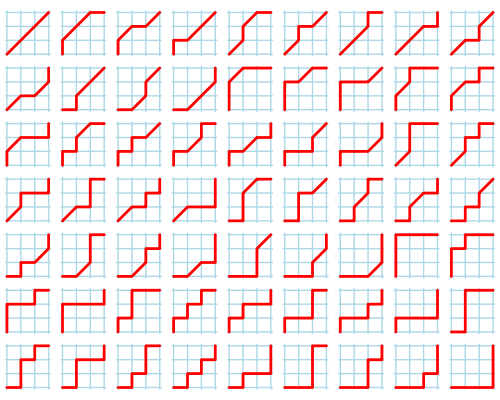
\includegraphics[width=0.5\textwidth,height=0.5\textwidth]{images/DelannoyNumbers.png}}
	\end{figure}
	
\textbf{\underline{Aim}:} To find $d_{n,m}$ \\ 

\textbf{Recurrence Relation:}\\ \\
Lets find a recurrence relation for $d_{n,m}$.
\\ 
A point (n,m) can be reached from three ways i.e. from (n-1,m), from (n-1,m-1) and from (n,m-1).
\\
Hence, the recurrence relation for $d_{n,m}$ will be,
\begin{equation}
\boxed{d_{n,m} = d_{n,m-1} + d_{n-1,m} + d_{n-1,m-1}}
\end{equation}

\textbf{Generating Function:}\\ \\
The generating function for this problem is,
\begin{equation}
\boxed{D(x,y) = \sum_{n,m \geq 0}d_{n,m}.x^n.y^m}
\end{equation}

We can observe that $d_{n,0}=d_{0,m}=1$.

$$D(x,y) = \sum_{n \geq 0,m=0}d_{n,0}.x^n + \sum_{n=0,m \geq 1}d_{0,m}.y^m + \sum_{n \geq 1,m \geq 1}d_{n,m}.x^n.y^m$$

$$D(x,y) = \sum_{n \geq 0,m=0}1.x^n + \sum_{n=0,m \geq 1}1.y^m + \sum_{n \geq 1,m \geq 1}d_{n,m}.x^n.y^m$$

We know that,
$$\sum_{n \geq 0}x^n = \frac{1}{1-x}$$

$$D(x,y) = \frac{1}{1-x} + \sum_{n=0,m \geq 1}y^m + \sum_{n \geq 1,m \geq 1}d_{n,m}.x^n.y^m$$

$$D(x,y) = \frac{1}{1-x} + y.\sum_{n=0,m \geq 1}y^{m-1} + \sum_{n \geq 1,m \geq 1}d_{n,m}.x^n.y^m$$


Let $(m-1)=h$,

$$D(x,y) = \frac{1}{1-x} + y.\sum_{n=0,h=0}y^h + \sum_{n \geq 1,m \geq 1}d_{n,m}.x^n.y^m$$

After renaming the variables,

$$D(x,y) = \frac{1}{1-x} + y.\sum_{n=0,m=0}y^m + \sum_{n \geq 1,m \geq 1}d_{n,m}.x^n.y^m$$

$$D(x,y) = \frac{1}{1-x} + y.\left(\frac{1}{1-y}\right) + \sum_{n \geq 1,m \geq 1}d_{n,m}.x^n.y^m$$

Using the recurrence relation from equation (18.81),

$$D(x,y) = \frac{1}{1-x} + \frac{y}{1-y} + \sum_{n \geq 1,m \geq 1}(d_{n,m-1} + d_{n-1,m} + d_{n-1,m-1}).x^n.y^m$$

$$D(x,y) = \frac{1}{1-x} + \frac{y}{1-y} + \sum_{n \geq 1,m \geq 1}d_{n,m-1} + \sum_{n \geq 1,m \geq 1}d_{n-1,m} + \sum_{n \geq 1,m \geq 1}d_{n-1,m-1}.x^n.y^m$$

$$D(x,y) = \frac{1}{1-x} + \frac{y}{1-y} + x.y.\sum_{n \geq 1,m \geq 1}d_{n-1,m-1}.x^{n-1}.y^{m-1} + \sum_{n \geq 1,m \geq 1}d_{n,m-1} + \sum_{n \geq 1,m \geq 1}d_{n-1,m}$$

Let $(n-1)=h~and~(m-1)=p$,
$$D(x,y) = \frac{1}{1-x} + \frac{y}{1-y} + x.y.\sum_{h \geq 0,p \geq 0}d_{h,p}.x^{h}.y^{p} + \sum_{n \geq 1,m \geq 1}d_{n,m-1} + \sum_{n \geq 1,m \geq 1}d_{n-1,m}$$

After renaming the variables,
$$D(x,y) = \frac{1}{1-x} + \frac{y}{1-y} + x.y.\sum_{n \geq 0,m \geq 0}d_{n,m}.x^{n}.y^{m} + \sum_{n \geq 1,m \geq 1}d_{n,m-1}.x^{n}.y^{m} + \sum_{n \geq 1,m \geq 1}d_{n-1,m}.x^{n}.y^{m}$$

From the equation (18.82),
\begin{equation}
D(x,y) = \frac{1}{1-x} + \frac{y}{1-y} + x.y.D(x,y) + \sum_{n \geq 1,m \geq 1}d_{n-1,m}.x^{n}.y^{m} +\sum_{n \geq 1,m \geq 1}d_{n,m-1}.x^{n}.y^{m}
\end{equation}

Consider the fourth term in the above equation,
$$\sum_{n \geq 1,m \geq 1}d_{n-1,m}.x^{n}.y^{m} = x.\sum_{n \geq 1,m \geq 1}d_{n-1,m}.x^{n-1}.y^{m}$$

Let $(n-1)=h$
$$x.\sum_{n \geq 1,m \geq 1}d_{n-1,m}.x^{n-1}.y^{m} = x.\sum_{h \geq 0,m \geq 1}d_{h,m}.x^h.y^m$$
After renaming the variables,

$$x.\sum_{h \geq 0,m \geq 1}d_{h,m}.x^h.y^m = x.\sum_{n \geq 0,m \geq 1}d_{n,m}.x^n.y^m$$

$$x.\sum_{n \geq 0,m \geq 1}d_{n,m}.x^n.y^m = x.\left(\sum_{n \geq 0,m \geq 0}d_{n,m}.x^{n}.y^{m} - \sum_{n \geq 0,m = 0}d_{n,0}.x^{n} \right)$$

$$x.\left(\sum_{n \geq 0,m \geq 0}d_{n,m}.x^{n}.y^{m} - \sum_{n \geq 0,m = 0}d_{n,0}.x^{n} \right) = x.\left(D(x,y)-\frac{1}{1-x} \right) $$ 
\\ \\
Substituting the above value in the equation (18.83),then

$$D(x,y) = \frac{1}{1-x} + \frac{y}{1-y} + x.y.D(x,y) + x.\left(D(x,y)-\frac{1}{1-x} \right) +\sum_{n \geq 1,m \geq 1}d_{n,m-1}.x^{n}.y^{m}$$

After rearranging the terms,

\begin{equation}
D(x,y) = 1 + \frac{y}{1-y} + x.y.D(x,y) + x.D(x,y) + \sum_{n \geq 1,m \geq 1}d_{n,m-1}.x^{n}.y^{m}
\end{equation}

Consider the last term of the above equation,

$$\sum_{n \geq 1,m \geq 1}d_{n,m-1}.x^{n}.y^{m} = y.\sum_{n \geq 1,m \geq 1}d_{n,m-1}.x^{n}.y^{m-1} $$

Let $p=(m-1)$,then 

$$y.\sum_{n \geq 1,m \geq 1}d_{n,m-1}.x^{n}.y^{m-1} = y.\sum_{n \geq 1,p \geq 0}d_{n,p}.x^{n}.y^{p}$$

After renaming the variables,

$$y.\sum_{n \geq 1,m \geq 0}d_{n,m}.x^{n}.y^{m} = y.\left(\sum_{n \geq 0,m \geq 0}d_{n,m}.x^n.y^m - \sum_{n=0,m \geq 0}d_{0,m}.y^{m} \right) $$

$$y.\left(\sum_{n \geq 0,m \geq 0}d_{n,m}.x^n.y^m - \sum_{n=0,m \geq 0}d_{0,m}.y^{m} \right) = y.\left(D(x,y) - \frac{1}{1-y} \right) $$

Substitute the above value in the equation (18.84),

$$D(x,y) = 1 + \frac{y}{1-y} + x.y.D(x,y) + x.D(x,y) + y.\left(D(x,y) - \frac{1}{1-y} \right)$$

$$D(x,y) = 1 + x.y.D(x,y) + x.D(x,y) + y.D(x,y) $$

After rearranging the terms,

$$D(x,y) = \frac{1}{1-x-y-xy} $$

$$D(x,y) = \left(\frac{1}{1-y}\right).\left(\frac{1}{1-\left(\frac{1+y}{1-y}\right).x}\right) $$

We know that,
$$\frac{1}{1-a.x} = \sum_{n \geq 0}a^n.x^n $$

$$D(x,y) = \left(\frac{1}{1-y}\right).\left(\sum_{n \geq 0}{\left(\frac{1+y}{1-y} \right)}^n.x^n \right) $$

The generating function is,
\begin{equation}
\boxed{D(x,y) = \left(\sum_{n \geq 0}{\frac{{(1+y)}^n}{{(1-y)}^{n+1}}}.x^n \right)}
\end{equation}

The required number $d_{n,m}$ is,\\

$$d_{n,m}~=~Coefficient~of~x^n.y^m~in~D(x,y)$$

$$d_{n,m}~=~Coefficient~of~y^m~in~{\frac{{(1+y)}^n}{{(1-y)}^{n+1}}}$$

$$d_{n,m}~=~Coefficient~of~y^m~in~ {(1+y)}^n.\left(\frac{1}{1-y}.\frac{1}{1-y}. \dots (n+1) times\right)$$

We know that,

$$\frac{1}{1-y} = 1+y+y^2+ \dots$$

$$d_{n,m}~=~Coefficient~of~y^m~in~{(1+y)}^n.\left((1+y+y^2+\dots).(1+y+y^2+\dots). \dots (n+1) times\right)$$

Let's say that a number $k \geq 0$ is taken, such that the term along with its coefficient $y^k$ comes from ${(1+y)^n}$ and the remaining term along with its coefficient $y^{m-k}$ comes from the (n+1) term product.\\

The coefficient of $y^k$ in ${(1+y)^n}$ is ${n \choose k}$.\\

Let $c_1,c_2,\dots,c_{n+1}$ be the degrees of x from the (n+1)-term product.\\

Finding out the coefficient of $y^{m-k}$ from the (n+1) term product is equivalent to count the number of ways of picking $c_i$'s such that $c_1+c_2+\dots+c_{n+1}=m-k$\\

The number of such pickings = ${{n+1+m-k-1} \choose {m-k}}$ = ${n+m-k} \choose {m-k}$ = ${n+m-k} \choose {n}$.\\

Therefore, the required number $d_{n,m}$ is,

$$d_{n,m} = \sum_{k \geq 0}{n \choose k}.{{n+m-k} \choose n}$$

Hence,
\begin{equation}
\boxed{Delannoy~Number~(D) = \sum_{k \geq 0}{n \choose k}.{{n+m-k} \choose n}}
\end{equation}























 

\Lecture{Jayalal Sarma}{Oct 21, 2020}{17}{Generating Functions(continued)}{Pragnya}{$\alpha$}{JS}

\section{Introduction}
In this section we'll see some examples of ordinary generating functions and get introduced to exponential generating functions.

\subsection{Example 3 : }
To show two combinatorial qualities are equal it sufficies to show that they have same generating functions. Consider the following,
$$ B_n(m) = \{(x_1, x_2, \dots x_n) ~|~ \forall i ~ x_i \in \Z , \sum |x_i| \leq m \}$$
let $b_{n,m} = |B_n(m)|$. Let's see properties of  $b_{n,m}$ :
\begin{enumerate}
    \item $b_{n, m} = \sum_{k=0}^n {n \choose k}{m \choose k} 2^k$.
    \item $b_{n, m} = b_{m, n}$. This can also be proved using bijection.
    \item $b_{n, m} = d_{m, n}$. 
\end{enumerate}
We'll prove property $3$ by showing they have same generating functions.
\begin{align*}
    B_{x,y} &= \sum_{n,m \geq 0} b_{n, m} x^n y^m\\
    &= \sum_{n,m \geq 0} (\sum_{k=0}^n {n \choose k}{m \choose k} 2^k) x^n y^m \\
    &= \sum_{n,m,k \geq 0}{n \choose k}{m \choose k} 2^k x^n y^m \\
    &= \sum_{k \geq 0} 2^k \sum_{n,m \geq 0} {n \choose k}{m \choose k} x^n y^m \\
    &= \sum_{k \geq 0} 2^k (\sum_{n \geq 0} {n \choose k} x^n)(\sum_{m \geq 0} {m \choose k} y^m) \\
B_{x, y}&= \sum_{k \geq 0} 2^k (x^k \sum_{n \geq 0} {n \choose k} x^{n-k})(y^k \sum_{m \geq 0} {m \choose k} y^{m-k})
\end{align*}
Consider $\frac{1}{(1-x)^{k+1}}$ : 
$$\frac{1}{(1-x)^{k+1}} = \frac{1}{(1-x)}.\frac{1}{(1-x)}. \dots \frac{1}{(1-x)} ~(k+1 ~times)$$
Coefficient of $x^{n-k}$ in $\frac{1}{(1-x)^{k+1}}$ is equivalent to no.of solutions of $a_1 + a_2 + \dots + a_{k+1} = n-k$ which is $ = {(n-k) + (k+1) -1 \choose n-k} = {n \choose k}$.
Hence
$$ \sum_{n \geq 0} {n \choose k} x^{n-k} = \frac{1}{(1-x)^{k+1}} $$
Similarly 
$$ \sum_{m \geq 0} {m \choose k} y^{m-k} = \frac{1}{(1-y)^{k+1}} $$
Substituting them in the above derived $B_{x, y}$ - 
\begin{align*}
    B_{x, y} &= \sum_{k \geq 0} 2^k x^k y^k \frac{1}{(1-x)^{k+1}} \frac{1}{(1-y)^{k+1}} \\
    &= \sum_{k \geq 0} (2xy)^k \frac{1}{(1-x)^{k+1}} \frac{1}{(1-y)^{k+1}} \\
    &= \frac{1}{(1-x)(1-y)} \sum_{k \geq 0} \frac{(2xy)^k}{(1-x)^k(1-y)^k} \\
    &= \frac{1}{(1-x)(1-y)} \sum_{k \geq 0} (\frac{(2xy)}{(1-x)(1-y)}) ^k \\
    &= \frac{1}{(1-x)(1-y)} \frac{1}{1- \frac{2xy}{(1-x)(1-y)}} \\
    &= \frac{1}{(1-x)(1-y) - 2xy} \\
    B(x, y) &=  \frac{1}{1 - x - y - xy} = D(x, y)
\end{align*}
Since $b_{n, m}$ and $d_{n, m}$ have same generating functions, $b_{n, m} = d_{n, m}$. Hence $b_{n, m}$ also satisfies recurrence relation of $d_{n, m}$ - 
$$ b_{n, m} = b_{n-1, m} + b_{n, m-1} + b_{n-1, m-1}$$


\subsection{Example 4 : Stirling number of second kind} 
As discussed in previous lectures, number of ways to partition set $\{1, 2, 3 \dots n \}$ into $k$ non-empty parts is called stirling number of second kind. Let's represent by $S_{n,k}$. It's recurrence relation is given by -  
$$S_{n, k} = S_{n-1, k-1} + k S_{n-1, k} $$
LHS : number of ways to partition set $\{1, 2, 3 \dots n \}$ into $k$ non-empty parts $ = S_{n, k}$ \\
RHS : \begin{enumerate}
\item If element $1$ occurs in a singleton set. No.of ways to partition remaining $n-1$ elements to $k-1$ sets $= S_{n-1, k-1}$.
\item If element $1$ doesn't occur in a singleton set. Then we can partition remaining $n-1$ elements to $k$ sets and add element $1$ to one of these $k$ sets $=  k S_{n-1, k}$
\end{enumerate}
We can also see that $S_{0,0} = 1 ,~ S_{n, 0} = 0 ,~ S_{0, k} = 0$.
%$S_{x, y} = {\sum_{n, k \geq 0} ^ {\infty} S_{n,k} x^n y^k}$ \\
%\begin{equation}
\begin{align*}
 S(x, y) &= {\sum_{n, k \geq 0} ^ {\infty} S_{n,k} x^n y^k} \\
&= S_{0,0}~x^0y^0 + {\sum_{n = 0, k \geq 1}^ {\infty} S_{0,k}~x^0y^k} + {\sum_{n \geq 1, k = 0}^ {\infty} S_{n,0}~x^n y^0} + {\sum_{n \geq 1, k \geq 1}^ {\infty} S_{n,k}~x^n y^k}  \\
 &= 1 + \sum_{n \geq 1 , k \geq 1} ^ {\infty} S_{n,k} ~ x^n y^k  \\
 &= 1 + \sum_{n \geq 1 , k \geq 1} S_{n-1, k-1}~ x^n y^k + \sum_{n \geq 1, k \geq 1} k S_{n-1, k}~ x^n y^k \\
 &= 1 + xy \sum_{n \geq 1, k \geq 1} S_{n-1, k-1} x^{n-1} y^{k-1} + x\sum_{n \geq 1, k \geq 1} k S_{n-1, k}~ x^{n-1} y^k \\
 &= 1 + xy~ S(x, y) + x \sum_{n \geq 0, k \geq 1} k S_{n, k}~ x^{n} y^k \\
 &= 1 + xy~ S(x, y) + \frac{\partial}{\partial y} S(x,y)
\end{align*}
Note : $\frac{\partial}{\partial y} S(x, y) = \sum_{n \geq 0, k \geq 1} k S_{n,k}~x^n y^{k-1}$ 


Consider $y^k$ coefficients on both sides : 
\begin{equation}
  \begin{split}
    LHS &= \sum_{n \geq 0} S_{n, k} x^n \\
    RHS &= x\sum_{n \geq 0} S_{n, k-1} x^n + xk \sum_{n \geq 0} S_{n, k}x^n
\end{split}  
\end{equation}
Equating LHS and RHS :
\begin{align*}
\sum_{n \geq 0} S_{n, k}~ x^n &= x\sum_{n \geq 0} S_{n, k-1} ~x^n + xk \sum_{n \geq 0} S_{n, k}~x^n \\
\sum_{n \geq 0} S_{n, k} ~x^n &= \frac{x}{1-xk}  \sum_{n \geq 0} S_{n, k-1}~ x^n   \\
&= \frac{x}{1-xk} \frac{x}{1-x(k-1)} \sum_{n \geq 0} S_{n, k-2}~ x^n \\
&= \frac{x}{1-xk} \frac{x}{1-x(k-1)} \dots \frac{x}{1-x(k-(k-1))}
\sum_{n \geq 0} S_{n, 0}~ x^n \\
&= \frac{x^k}{(1-x)(1-2x)\dots (1-kx)} \times 1 ~( Note : S_{0,0} = 1, S_{n, 0} = 0) \\
\sum_{n \geq 0} S_{n, k}~ x^n &= x^k \times (\frac{A_1}{1-x} + \frac{A_2}{1-2x} + \dots +  \frac{A_k}{1-kx})
\end{align*}
Solving for $A_1, A_2, \dots A_k $ we'll get $A_r = (-1)^{k-r} \frac{r^{k-1}}{(r-1)! (k-r)!}$. \\
$S_{n,k}$ is the coefficient of $x^n$ in RHS. i.e., 
\begin{align*}
S_{n,k} &= coeff~ of ~x^n ~in~ x^k \times (\frac{A_1}{1-x} + \frac{A_2}{1-2x} + \dots +  \frac{A_k}{1-kx}) \\
&= coeff ~ of ~ x^{n-k} ~ in ~ \sum_{r=1}^k \frac{A_r}{1-rx}
\end{align*}
Coefficient of $x^{p}$ in $\frac{1}{1-rx} = r^p$. hence,
\begin{align*}
S_{n,k} &= \sum_{r=1}^k A_r r^{n-k} \\
&= \sum_{r=1}^k (-1)^{k-r} \frac{r^{k-1}}{(r-1)! (k-r)!} ~ r^{n-k}\\
S_{n,k} &= \sum_{r=1}^k (-1)^{k-r} \frac{r^{n}}{(r-1)! (k-r)!}
\end{align*}
The above expression is Stirling number of second kind
%\end{equation}
%$$ = S_{0,0}~x^0y^0 + {\sum_{n = 0, k \geq 1}^ {\infty} S_{0,k}~x^0y^k} + {\sum_{n \geq 1, k = 0}^ {\infty} S_{n,0}~x^ny^0} + {\sum_{n \geq 1, k \geq 1}^ {\infty} S_{n,k}~x^ny^k} $$ \\
%$&= 1 + \sum_{\substack{n \geq 1 \\ k \geq 1}} ^ {\infty} S_{n,k} ~ x^n y^k$

\section{Exponential generating functions}
In ordinary generating functions we associate sequence, ${(a_n)}_{n \geq 0}$ with $G(x) = \sum_{n \geq 0} a_n x^n$. In $G(x)$ we chose basis $\{ 1, x, x^2, x^3 \dots\}$ for set of all polynomials in one variable. But there are many other basis for set of polynomials, like $\{1, x, x(x-1), x(x-1)(x-2), \dots\}$. We chose basis $\{ 1, x, x^2, x^3 \dots\}$ because it has combinatorial meaning. Other such meaning full basis are $\{\frac{x^n}{n!}\}_{n \in \N}$, $\{e^{-x} \frac{x^n}{n!}\}_{n \in \N}$ and $\{\frac{1}{n^x}\}_{n \in \N}$. In this lecture we'll explore exponential generating functions which use basis $\{\frac{x^n}{n!}\}_{n \in \N}$ . \\
So  ${(a_n)}_{n \geq 0}$ is associated with $E(x) = \sum_{n \geq 0} a_n \frac{x^n}{n!}$ . Let's see a few examples - 
\begin{align*}
(1, 1, 1, \dots ) &\xrightarrow[generating function]{exponential} \sum_{n \geq 0} \frac{x^n}{n!} = e^x    \\
&\xrightarrow[generating function]{ordinary} \sum_{n \geq 0} x^n = \frac{1}{1-x} \\
(1!, 2!, 3!, \dots) &\xrightarrow[generating function]{exponential} \sum_{n \geq 0} n! \frac{x^n}{n!} = \sum_{n \geq 0} x^n = \frac{1}{1-x}
\end{align*}
$\frac{1}{1-x}$ is ordinary generating function(ogf) of $(1, 1, 1, \dots )$ and exponential generating function(egf) of $(1!, 2!, 3!, \dots )$.\\
\\
\textbf{\Large {Operations of EGF}}
\begin{enumerate}
\item{\textbf{Addition :} } It's similar to ogf.
    \begin{align*}
        \{a_n\}_{n \geq 0} &\xrightarrow[]{egf} E(x) \\
        \{b_n\}_{n \geq 0} &\xrightarrow[]{egf} F(x) \\
        \{a_n + b_n \}_{n \geq 0} &\xrightarrow[]{egf} E(x) + F(x) \\
    \end{align*}
\item {\textbf{Shifting :} } Multiplying ogf by $x$ shifts the sequence to left as seen in earlier lectures.  
    \begin{align*}
        \{a_0, a_1, a_2 \dots \} &\xrightarrow[]{egf} E(x) \\
        \{0, a_0, a_1, a_2 \dots \} &\xrightarrow[]{egf} xE(x) \\
    \end{align*}
Differentiating egf function will shift the sequence to right.
\begin{gather*}
    \{a_0, a_1, a_2 \dots \} \xrightarrow[]{egf} ~~ E(x) \endline
        \{a_1, a_2, a_3 \dots \} \xrightarrow[]{egf} \frac{d}{dx} E(x) \\
        \frac{d}{dx} E(x) = \sum_{n \geq 1} a_n~ \frac{n. x^{n-1}}{n!} = \sum_{n \geq 1} a_n~ \frac{x^{n-1}}{(n-1)!} =  \sum_{n \geq 0} a_{n+1}~ \frac{x^{n}}{n!}
\end{gather*}
\item {\textbf{Multiplication :} }   EGFs are used if the sequence counts labelled structures like permutations, derangements and partitions. Let $(a_n)_{n \geq 0}$, $(b_n)_{n \geq 0}$ count arrangements  of type $A$ and type $B$ respectively using $n$ labelled objects. If we want to count type $C$ arrangements, that can be obtained by a unique split of $n$ objects into two sets and then arranging first set according to type $A$ and second set according to type $B$ - \\
 No.of arrangements of type $C$ of size $n, c_n = \sum_{k=0}^n {n \choose k} a_k b_{n-k}$.\\
 Now Let's see how multiplication of $A(x)$(egf of $A$) and $B(x)$(egf of $B$) is useful 
 \begin{align*}
     A(x).B(x) &= (\sum_{n=0}^{\infty} a_n \frac{x^n}{n!})(\sum_{n=0}^{\infty} b_n \frac{x^n}{n!}) \\
     &= \sum_{n=0}^{\infty}(\sum_{k=0}^{n} \frac{a_k}{k!}.\frac{b_{n-k}}{(n-k)!}) x^n \\
     &= \sum_{n=0}^{\infty}(\sum_{k=0}^{n} \frac{n!}{k!(n-k)!} a_k b_{n-k}) \frac{x^n}{n!} \\
     &= \sum_{n=0}^{\infty}(\sum_{k=0}^{n} {n \choose k} a_k b_{n-k}) \frac{x^n}{n!} \\
     &= \sum_{n=0}^{\infty} c_n \frac{x^n}{n!} \\
     A(x).B(x) &= C(x)
 \end{align*}
 
 Now Let's see few examples of egf 
 \subsection{Derangements } Recall that we've discussed derangements in PIE and recurrence relations. Now let's derive it using egf. Let $D_n$ represent set of derangements of $n$ objects and let $d_n = |D_n|$. we can see that $d_0 = 1 ,~ d_1 = 0,~ d_2 = 1$. Recall the recurrence relation : $$ d_{n+2} = (n+1)(d_{n+1} + d_n)$$
 \begin{align*}
     D(x) &= \sum_{n=0}^{\infty} d_n \frac{x^n}{n!} \\
     D'(x) &= \sum_{n=0}^{\infty} d_{n+1} \frac{x^n}{n!} ~(by ~shifting ~operation)\\
     &= \sum_{n=1}^{\infty} n(d_n + d_{n-1}) \frac{x^n}{n!} \\
     &= \sum_{n=1}^{\infty} nd_n \frac{x^n}{n!} + \sum_{n=1}^{\infty} nd_{n-1} \frac{x^n}{n!} \\
     &= x \sum_{n=1}^{\infty} d_n \frac{x^{n-1}}{(n-1)!} + x \sum_{n=1}^{\infty} d_{n-1} \frac{x^{n-1}}{(n-1)!} \\
     &= x \sum_{n=0}^{\infty} d_{n+1} \frac{x^n}{n!} + x \sum_{n=0}^{\infty} d_n \frac{x^n}{n!} \\
     D'(x) &= xD'(x) + xD(x) \\
     (1-x)D'(x) &= xD(x) \\
     \frac{D'(x)}{D(x)} &= \frac{x}{1-x} = \frac{1}{1-x} - 1
 \end{align*}
Integrating on both sides
     $$\ln{D(x)} = \ln{(1-x)} - x + c$$
Since $D(0) = d_0 = 1 \implies c=0$.
    $$\ln{D(x)} = \ln{(1-x)} - x$$
    $$D(x) = \frac{e^{-x}}{1-x} = \sum_{n=0}^{\infty} d_n \frac{x^n}{n!}$$
To get $d_n$ we need coefficient of $\frac{x^n}{n!}$ in LHS.
$$e^{-x} \frac{1}{1-x} = (\sum_{n=0}^{\infty} (-1)^n \frac{x^n}{n!})(\sum_{n=0}^{\infty} n! \frac{x^n}{n!})$$
Coefficient of $\frac{x^n}{n!}$ by multiplication property = $\sum_{k=0}^{n} {n \choose k} a_k b_{n-k}$
\begin{align*}
    d_n = \sum_{k=0}^{n} {n \choose k} (-1)^{n-k} k!  
    = \sum_{k=0}^{n} (-1)^{n-k} k! {n \choose k}
\end{align*}
$d_n$ is count of derangements of $n$ objects.

\subsection{Bell Numbers}
Let $S_{n,k}$ represent number of ways of partitioning \{$1, 2 ,3 \dots n $\} into $k$ non empty blocks and $B_n$ represent number of ways of partitioning \{$1, 2 ,3 \dots n $\} ($B_0 = 1$). By definitions, 
$$B_n = \sum_{k=0}^n S_{n,k}$$
Equivalent intrepretation :  Consider a number whose prime factorization is square free i.e., $k \in \N$ such that $k = p_1p_2 \dots p_n$ where $\{p_1, p_2, \dots p_n\}$ are distinct primes. Number of ways of writing $k$ as product of natural numbers $\geq 2 = $ number of ways of partitioning  $\{p_1, p_2, \dots p_n\}$  $= B_n$. \\
Recurrence Relation : 
 $$ B_n = \sum_{k=0}^{n-1} {{n-1} \choose k} B_k $$ 
% LHS : Number ways of partitioning  \{$1, 2 ,3 \dots n $\}. \\
% RHS : \begin{parts}
% \item If $1$ occurs in singleton set. No.of such partitions  = $B_{n-1}$
% \item If $1$ occurs in set with two elements. No.of ways element can be chosen $ = n-1$.No.of such partitions  = ${{n-1} \choose 1}B_{n-2}$.
% \item $1$ occurs in set with $k+1$ elements. No.of ways elements in this set can be chosen $ = {n-1 \choose k}$. No.of such partitions  = ${{n-1} \choose k}B_{n-(k+1)}$.
% \end{parts}
% Hence total $= \sum_{k=0}^{n-1} {{n-1} \choose k} B_{n-k-1}  = \sum_{k=0}^{n-1} {{n-1} \choose n-k-1} B_{n-k-1} = \sum_{n-k-1=0}^{n-1} {{n-1} \choose k} B_{k} = \sum_{k=0}^{n-1} {{n-1} \choose k} B_{k} $ \\
 Let's derive closed form expression for $B_n$ :
 \begin{align*}
     B(x) &= \sum_{n=0}^{\infty} B_n \frac{x^n}{n!} \\
     B'(x) &= \sum_{n=0}^{\infty} B_{n+1} \frac{x^n}{n!} ~(by ~ shifting ~rule) \\
     &= \sum_{n=0}^{\infty} (\sum_{k=0}^{n} {n \choose k} B_k) \frac{x^n}{n!} \\
     &= \sum_{n=0}^{\infty} (\sum_{k=0}^{n} {n \choose k}. ~1 B_k) \frac{x^n}{n!} \\
     &= (\sum_{n=0}^{\infty} B_n \frac{x^n}{n!})(\sum_{n=0}^{\infty} 1 \frac{x^n}{n!}) ~(by ~ multiplication ~rule) \\
     B'(x) &= B(x) . e^x \\
     \frac{B'(x)}{B(x)} &= e^x
 \end{align*}
 Integrating on both sides 
 $$\ln{B(x)} = e^x + c$$
 Since $B(0) = B_0 = 1 \implies c = -1$. Hence,
 %$$ B(x) = e^{e^x - 1} = \frac{e^{e^x}}{e}$$
 \begin{align*}
     B(x) &= e^{e^x - 1} \\
     &= \frac{e^{e^x}}{e} \\
     &= \frac{1}{e} (\sum_{k=0}^{\infty} \frac{(e^x)^k}{k!}) \\
     &= \frac{1}{e} (\sum_{k=0}^{\infty} \frac{e^{kx}}{k!}) \\
     &= \frac{1}{e} (~\sum_{k=0}^{\infty} \frac{1}{k!}~ (\sum_{n=0}^{\infty} \frac{(kx)^n}{n!})~) \\
     &= \frac{1}{e} (~\sum_{n=0}^{\infty} \frac{x^n}{n!}~ (\sum_{k=0}^{\infty} \frac{k^n}{k!})~)\\
B(x)&= \sum_{n=0}^{\infty} \frac{1}{e} (\sum_{k=0}^{\infty} \frac{k^n}{k!}) \frac{x^n}{n!} \\
    B_n &= \frac{1}{e} (\sum_{k=0}^{\infty} \frac{k^n}{k!})
 \end{align*}
 We've derived closed form expression for bell number. Above expression for $B_n$ is also called as Dobinski's formula.
 
\end{enumerate}

\Lecture{Jayalal Sarma}{Oct 19, 2020}{18}{Introduction to Ramsey Numbers}{Shivlal Gangesh}{$\alpha$}{JS}
\section{Introduction}
Till now we have seen advanced versions of the discrete mathematics topics we already know. Now we are going to get into Extremal combinatorics. Here we are interested in questions of the form 
\begin{itemize}
\item \textit{If this structure appears, then what is the minimum/maximum size of the object?}
\item \textit{If the size is at least this much , then what kind of structures appear in the object?}
\item \textit{What is the minimum size of the collection such that it is guaranteed to have certain property?}
\end{itemize}
In general we are interested in the extreme behaviors in combinatorics. The classic example we start with is an extension to an example that we have done in the beginning of the course as an Application of Pigeon Hole Principle.
\section{Starting Point} \label{R(3,3)}
\begin{theorem}
Six people meet in a party. Then either there exist three people who are friends with each other or there exist three people who are strangers with each other.(Note : Any two people can either be friends or strangers)
\end{theorem}
We are interested in proving the above statement. Lets look into two different approaches
\subsection{Model 1 (Using Cliques and Independent Sets)}
\begin{description}
   \item[Model] Let us represent the problem as a $6$ vertex graph $G(V,E) $with each person corresponding to a vertex. $(u,v) \in E$ if and only if person $u$ is a friend of person $v$.
In this Model the original statement can be reformulated as
\item[Statement]
\textit{Any graph on $6$ vertices must either have a clique on $3$ vertices or an independent set on $3$ vertices.
\item}
\begin{proof}
 Consider any vertex $v$ in the graph G, without loss of generality we can assume that the degree of $v$ is greater than or equal to $3$  because suppose it is not the case then consider $\overline{G}$ ; as $\textrm{Cliques in }G \leftrightarrow \textrm{Independent Sets in } \overline{G} $.\\
 Let the $3$ neighbours of $v$ be $a$, $b$ and $c$. Consider the two exhaustive cases :
 \begin{description}
    \item[Case 1 : There are no edges among $a$, $b$ and $c$]
    $ $ \newline
    Here we have $\{a, b, c\}$ as the 3-Independent Set
    \item[Case 2 : There is at least one edge among $a$, $b$ and $c$ ]
    $ $ \newline
    Let $(a,b) \in E$ be that edge, then we have $\{v, a, b\}$ as the 3-clique
 \end{description}
Therefore the given statement holds true.
\end{proof}
\item[Proof for tightness]
To prove that this is tight we need to show there is a graph with $5$ vertices such that it does not have 3-clique and 3-Independent Set. Given below is one such  example
\begin{figure}[h!]
    \centering
    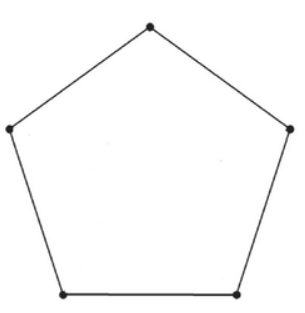
\includegraphics[width=0.2\linewidth]{images/r33counter_example.png}
    \caption{5-vertex graph with no 3-clique and no 3-Independent Set}
\end{figure}
\end{description}
\subsection{Model 2 (Using Graph Edge colouring)}
\begin{description}
   \item[Model]
   Let us represent the problem as 2-edge coloring of a $K_6$ graph with each vertex corresponding to a person. Color the edge $(u,v)$ with \textit{red} if $u$ and $v$ are friends, color it with \textit{blue} if $u$ and $v$ are strangers.
In this Model the original statement can be reformulated as
\item[Statement]
\textit{For any 2-edge colouring of $K_6$, there must exist either  a red $K_3$  or a blue $K_3$ }
\item
\begin{proof}
 Consider any Red,Blue-edge coloring of $K_6$. Consider any vertex $v$, the degree of $v$ is $5$ as the graph is a complete graph. By Pigeon Hole Principle , $v$ must have either $3$ red edges incident on it or $3$ blue edges incident on it. Consider the case when $v$ is incident on with $3$ red edges. Let the 3 neighbours of $v$ be $a$, $b$ and $c$.  Now there are 2 cases :
 \begin{description}
    \item[Case 1 : There is no red colored edge among $(a,b)$, $(b,c)$ and $(c,a)$ ]
    $ $ \newline
    Then all the three edges $(a,b)$, $(b,c)$ and $(c,a)$ are colored blue. Therefore $\{a, b, c\}$ forms a blue $K_3$
    \item[Case 2 : There is at least one red colored edge among $(a,b)$, $(b,c)$ and $(c,a)$ ]
    $ $ \newline
    Let $(a,b)$ be the red colored edge, then $\{v, a, b\}$ forms a red $K_3$
 \end{description}
 Therefore the given statement holds true.
\end{proof}
\item[Proof for tightness]
To prove that this is tight we need to show there is a 2-edge coloring of $K_5$ Such that it does not have red $K_3$ and blue $K_3$. Given below is one such  example
\begin{figure}[h!]
    \centering
    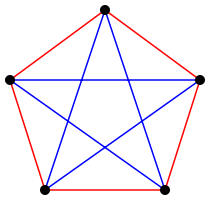
\includegraphics[width=0.2\linewidth]{images/k5counter_example.png}
    \caption{2-edge coloring of $K_5$ with no red $K_3$ and no blue $K_3$}
\end{figure}
\end{description}

Generalizing the above problem with arbitrary red $k_p$ and blue $k_q$ has been extensively studied by Ramsey and has led to the definition of Ramsey numbers.
\section{Ramsey numbers}
\begin{definition}[Ramsey number]
The Ramsey number denoted by $R(p,q)$ is the minimum number of vertices say $n$ such that any 2-edge coloring of $K_n$ must have either a red $K_p$ or a blue $K_q$.\\
(\textbf{Or equivalently as})\\
The minimum number of vertices ($n$) such that any graph on $n$ vertices must either have a clique on $p$ vertices or an independent set on $q$ vertices.
\end{definition}

\subsection{Some Observations}
\begin{property}
$R(3,3)=6$
\end{property}
This is the direct formulation of the example we have done previously in \ref{R(3,3)}
\begin{property}
$R(p,q) = R(q,p)$
\end{property}
The colors \textit{red} and \textit{blue} are just placeholders for two colors, thus swapping the colors will still preserve the Ramsey number property. Therefore $R(p,q) = R(q,p)$.
\begin{property}
$\forall l \geq 1 \quad R(l,1) = 1$
\end{property}
The existence of a blue $K_1$ is nothing but the presence of single vertex and any graph with a single vertex satisfies this property. Therefore $R(l,1) = 1$


\section{Existence of R(p,q)}
The Proof for the existence of $R(p,q)$ is due to Erdős–Szekeres. The existence was proved by providing an upper bound as a recurrence relation as follows :
\begin{theorem}
$$\forall p,q \geq 2 \quad R(p,q) \; \leq \; R(p,q-1) + R(p-1,q) $$
\end{theorem}
\begin{proof}
 Let us prove this by mathematical induction on $n$ where $n=p+q$.
 \begin{description}
    \item[Idea] To show the upper bound for $R(p,q) \leq n$ , we must argue that for any 2-edge coloring of $K_n$ there exist a red $K_p$ or blue $K_q$

   \item[Base case] $p=q=2$
$$R(2,2) \leq  R(2,1) + R(1,2)  $$
$$2 \leq 1+1$$
Hence it holds true for the base case.
   \item[Induction Hypothesis]
Assume the recurrence relation is true for $n<l$. Then we need to prove it for $n=l$. Let $n=R(p-1,q)+R(p,q-1)$. Let $w$ be any vertex in $G$ ($K_n$) and consider any $2$ -edge coloring of $G$. Let $H_1$ be the subgraph of $G$ formed from the vertices sharing a red-edge with $v$ and $H_2$ be the the subgraph of $G$ formed from the vertices sharing a blue-edge with $v$.
\begin{description}
   \item[Case 1 : There are at least $R(p-1,q)$ many red edges incident on vertex $w$]
   $ $ \newline
   $H_1$ is a complete graph on $R(p-1,q)$ vertices with 2-edge coloring. By definition and Induction Hypothesis we have that there exist a red $K_{p-1}$ or blue $K_q$ in $H_1$. So in graph $G$ (along with vertex $w$) there exist a red $K_p$ or blue $K_q$
   \item[Case 2 : There are at least $R(p,q-1)$ blue edges incident on vertex $w$]
      $ $ \newline
      $H_2$ is a complete graph on $R(p,q-1)$ vertices with 2-edge coloring. By definition and Induction Hypothesis we have that there exist a red $K_p$ or blue  $K_{q-1}$ in $H_2$. So in graph $G$ (along with vertex $w$) there exist a red $K_p$ or blue $K_q$.
\end{description}
   \end{description}
   
\end{proof} 
   
\Lecture{Jayalal Sarma}{Oct 21, 2020}{19}{Computing Ramsey Numbers and Multidimensional Ramsey numbers}{Shivlal Gangesh \& Reetwik Das}{$\alpha$}{JS}
\section{Generalizing Ramsey numbers}
\begin{definition}[3-dimensional Ramsey numbers]
$R_3(p,q,r)$ is the minimum number $n$, such that any 3-edge coloring $K_n$ must have either a red $K_p$ or a blue $K_q$ or a green $K_r$
\end{definition}
\begin{definition}[$k$-dimensional Ramsey numbers]
$R_k(s_1,s_2,\cdots ,s_k)$ is the minimum number of vertices $n$ such that for any $k$-edge coloring of $K_n$  there must exist an $i$ such that there is a $K_{s_i}$ of colour $i$
\end{definition}

\section{Some Observations}
\begin{property}
$R(2,p)=p$
\end{property}
\begin{proof}
$ $ 
 \begin{description}
    \item[Case1 : $R(2,p) \leq p$]
    $ $ \newline
    Any 2-coloring of $K_p$ must have either a red $K_2$ or blue $K_p$. This is true because either there can exist a red edge (red $K_2$) or no red edge (blue $K_p$) in $K_p$
    \item[Case 2 : $R(2,p) \geq p$]
    $ $ \newline
    There exist a 2-coloring of edges of $K_{p-1}$ such that no red $K_2$ exists and no blue $K_p$ exists. Coloring all the edges of $K_{p-1}$ with blue will result in no red $K_2$ and no blue $K_p$ in $K_{p-1}$
 \end{description}
\end{proof}
\begin{claim}
$$ R(p,q) \leq {p+q-2 \choose p-1} $$
\end{claim}
\begin{proof}
 \begin{align*}
     R(p,q) &\leq  R(p,q-1) + R(p-1,q) && \textrm{(Erdos-Szekeres recurrence relation)} \\
     &\leq {p+(q-1)-2 \choose p-1} + {p-1+q-2 \choose p-2} \\
     &\leq {p+q-3 \choose p-1} + {p+q-3 \choose p-2} \\
     &\leq {p+q-2 \choose p-1}  && ({n+1 \choose k+1} = {n \choose k+1} +{n \choose k})
 \end{align*}

\end{proof}
\section{Explicit Computation of R(3,4)}
We don't know the exact values of Ramsey numbers for higher values as their computation becomes very hard. There is this famous saying by Paul Erdos on the difficulty of computing Ramsey numbers that
\begin{description}
   \item[Paul Erdos on Ramsey numbers] 
   $ $ \newline
\textit{   "Suppose aliens invade the earth and threaten to obliterate it in a year's time unless human beings can find the Ramsey number for red five and blue five. We could marshal the world's best minds and fastest computers, and within a year we could probably calculate the value. If the aliens demanded the Ramsey number for red six and blue six, however, we would have no choice but to launch a preemptive attack."}
\end{description}
 So let us now try to calculate the value of $R(3,4)$. 
 \begin{claim}
 $$ R(3,4) = 9 $$
 \end{claim}
 \begin{proof}
 $ $
 Consider any 2-coloring of $K_9$ and call it as $G$. We need to prove that $G$ has either a red $K_3$ or a blue $K_4$. Any vertex in $G$ can have it's incident edges as one of the three cases below
  \begin{itemize}
  \item \textbf{Case 1 : }There are at least $4$ red edges going out of the vertex
  \item \textbf{Case 2 : }There are at least $6$ blue edges going out of the vertex
  \item \textbf{Case 3 : }There are exactly $3$ red edges and $5$ blue edges going out of the vertex
  \end{itemize}
 However note that not all vertices in $G$ come under \textbf{Case 3} because, if so then the total sum of degrees of all vertices becomes odd which is not possible. So let $v$ be a vertex in $G$ which does not fall under \textbf{Case 3}. Then
 \begin{description}
    \item[Case 1 : There are at least 4 red edges going out of $v$ ]
    $ $ \newline
    Let $H_1$ be the subgraph of $G$ formed from the four vertices which are sharing the red edge with $v$.  Since we know that $R(2,4)=4$, $H_1$ with 4 vertices must have a red $K_2$ or a blue $K4$, So along with vertex $v$, $G$ must have a red $K_3$ or a blue $K_4$.
    \item[Case 2 :There are at least 6 blue edges going out of $v$]
    $ $ \newline
    Let $H_2$ be the subgraph of $G$ formed from the six vertices which are sharing the blue edge with $v$. Since we know that $R(3,3)=6$, $H_2$ with 6 vertices must have a red $K_3$ or a blue $K3$, So along with vertex $v$, $G$ must have a red $K_3$ or a blue $K_4$.
    \item[Proof for tightness]
    $ $ \newline
    To prove that $9$ is tight, we need to show that there is a 2-coloring of $K_8$ such that it does not have red $K_3$ or blue $K_4$. Given below is one such  example
\begin{figure}[h!]
    \centering
    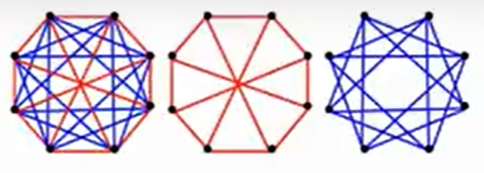
\includegraphics[width=0.5\linewidth]{images/R34counter_example.png}
    \caption{2-coloring of $K_8$ with no red $K_3$ and no blue $K_4$}
\end{figure}
 \end{description}
  
 \end{proof}
 As the values $p$, $q$ increases we can only calculate the range of the Ramsey number. The following is a table with value or range of Ramsey numbers for the first few natural numbers.
 \begin{figure}[h!]
    \centering
    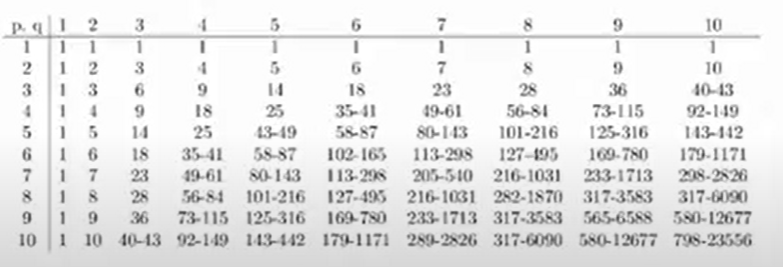
\includegraphics[width=1\linewidth]{images/RamseyTable.png}
    \caption{Table for $R(p,q)$}
\end{figure}

% Reetwik Started from here

\section{Multidimentional Ramsey numbers}
\begin{definition}
$R_k(S_1,S_2,..S_k)$ is mininum number $n$ such that any $k$-edge coloring of $K_n$ must have $K_{S_i}$ of color $i$ for some $i \in \{1,2..k\}$
\end{definition}
We need to show that why should exist $R_k(S_1,S_2,..S_k)$.
\begin{claim}
$$R_k(S_1,S_2,..S_k) \leq R_{k/2}(R(S_1,S_2), R(S_3,S_4).... R(S_{k-1},S_k))$$
\end{claim}
\begin{proof}
Let $n =  R_{k/2}(R(S_1,S_2), R(S_3,S_4).... R(S_{k-1},S_k))$\\
Consider $K_n$ and any K-edge coloring of the edges of $K_n$\\

We need to show that $\exists S_1$ clique of color 1 or $S_2$ clique of color 2.\\
Consider colors paired up and rename them $\{1,2\} = 1, \{3,4\} = 2, ... \{k-1,k\} = k/2$ \\
By the definition of $R_{k/2}$ we are guaranteed $\exists i$ such that $\exists$ a clique of size $R(S_{2i-1},S_{2i})$ of color $i$.\\

After we uninterpret the color $i$ as the original pair of colors we get a 2-coloring of the clique that we have $R(S_{2i-1},S_{2i})$\\
By the definition of $R_2$ we know that $\exists$ a $S_{2i-1}$ clique of color $2i-1$ or $S_{2i}$ clique of color $2i$.
\end{proof}

\section{Fermat's last theorem}
We know from Pythagoras theorem that $x^2 +y^2 = z^2$ has integral solutions. But we want to know if this equation has any integral solutions for any power greater than $2$.
\begin{theorem}
$x^n +y^n = z^n$ doesn't have any integral solutions $\forall n>2$.
\end{theorem}

\Lecture{Jayalal Sarma}{Oct 22, 2020}{20}{Finite fields}{Reetwik Das}{$\alpha$}{JS}

\subsection{Finite fields}
$x^n +y^n = z^n$ does have integeral solutions for finite fields such as for $Z_p$.\\
$Z_p = \{0,1,....p-1\}$ and addition and multiplication are $modulo$ $p$ within this field.\\

\begin{definition}
$Z_p^*$ is a cyclic group $\{1,2,3....p-1\}$
\end{definition}

\begin{claim}
If $p$ is a prime then $Z_p^*$ is generated by a single element, and the element is known as the generator.
\end{claim}

Fermat's last theorem is completely algebraic to connect it to coloring we need a tool.
\begin{theorem}
\textbf{Schur's theorem :} If $r \geq 0$ positive integer then. $\exists$ integer $S(r)$ such that if we color $\{1,2,....S(r)\}$ vertices with $r$ colors then $\exists x,y,z$ in the set and $x+y =z$
\end{theorem}
\begin{proof}
Given an $r$, Let $S(r) = R_r(3,3,3,...3)$\\
Consider $K_n$, $n = S(r)$ by the definition if we color the edges of $K_n$ using $r$ colors then we are guaranteed a monochromatic $K_3$.\\
We are given a coloring $\{1,2,...S(r)\}$\\
Define a coloring for edges in $K_n$.\\
Associate vertices of $K_n$ with elements in $\{1,2,...S(r)\}$ \\
$\forall a,b\in V$ the color of edge $(a,b) $ = color of $|a-b|$\\

Let $\{\alpha, \beta,\gamma\}$ be the vertices of the monochromatic triangle.
Let $x = \alpha - \beta$, $y = \beta - \gamma$ and $z = \alpha - \gamma$ then $x,y,z$ have the same color.
It also satifies the equation $x+y =z$.
 
\end{proof}

\begin{theorem}
$\forall m \exists q$ such that $\forall p\geq q$ in $Z_p$ ($p$ is a prime) \\
$x^m +y^m = z^m$ has a solution.
\end{theorem}
\begin{proof}
Given $m$ from $ x^m +y^m = z^m$\\
$p=q=S(m)+1$ by Schur's theorem any coloring of $\{1,2...q\}$ must have a triplet $a+b = c$.\\
$Z_p = {0,1,2...q-1}$\\
Let $g$ be the generator of $Z_p$ then every non-zero element in $Z_p = g^k$ for some $k$.\\

Assign the coloring $\{1,2...q\}$ as follows :\\
$\forall x \in Z_p^*,  x=g^{mi+j}$ and $color(x)= j = k (mod m)$\\

By Schur's theorem, $\exists a,b,c$ such that $a+b=c$ and all have the same color.\\
$$g^{mi_a+j} + g^{mi_b+j} = g^{mi_c+j}$$
$$(g^{i_a})^m + (g^{i_b})^m = (g^{i_c})^m$$
and we have the solution for $x^m +y^m = z^m$. 
\end{proof}

\subsection{Lower bounds for Ramsey numbers}
\begin{claim}
$$\forall k, R(k,k) > 2^{k/2}$$
\end{claim}
\begin{proof}
Suffices to show that $n = 2^{k/2}$, $\exists$ a 2-coloring of the edges of $K_n$ such that there is no monochromatic $K_k$ in it.\\

Fix $m = 2^{k/2}$ there are $n\choose 2$ many edges.\\
A coloring is said to be bad if $\exists$ no monochromatic $K_k$ in it.\\

\textbf{Probabilistic method :}\\
For every edge, assign red/blue color with probability 1/2 each.\\
if we show that the probability[coloring is bad]$ > 0$ then this means $\exists$ a bad coloring.\\

Suffices to show that the Pr[coloring is good] $<1$\\
Pr[$\exists K_k$ which is monochromatic] $\leq \Sigma_{S \subseteq K_k,|S|=k}$ Pr[S is monochromatic]\\
$ = {n\choose k}$ Pr[S is monochromatic]
$$ = {n\choose k} \frac{2}{2^{k\choose 2}}$$
$$= {n\choose k} 2^{1-{k\choose2}}$$
$$ =\frac{n(n-1)...(n-k+1)}{k!} \frac{2^{1+k/2}}{2^{k^2/2}}$$
$$ \leq \frac{n^k}{k!} \frac{2^{1+k/2}}{2^{k^2/2}}$$
$$= \frac{2^{1+k/2}}{k!} < 1$$
\end{proof}

\Lecture{Jayalal Sarma}{Oct 26, 2020}{23}{Extremal Problems In Graphs-Three Proofs,Mantels Theorem}{Praharsh Allada}{$\alpha$}{JS}
\section{Introduction}
This week we are going to look at some extremal problems in graphs.The techniques we use to Solve the problems are more important than the problems themselves.In fact we will look at multiple ways of proving the same statement using different techniques to prove.\\
\textbf{Example 1:-}\\
Suppose an Undirected Graph G ,does not have triangle(no $k_3$), what is the maximum number of edges the graph G can have?\\
(OR)\\ 
What is the minimum number of edges that a graph G with n vertices should have so that it always contains at least 1 triangle?\\
\textbf{Solution:-}\\
The graph can be divided Into 2 sets of vertices of size $\frac{n}{2}$ and from all the possible edges from one set to another.In this case we put in $\frac{n^2}{4}$ edges.(From a little thought and AM$ \geq $GM we can see that the highest number of edges are produced when each set contains $\frac{n}{2}$ vertices).The answer to the question is this the best we can do is yes,this is the best that we can do, we can not have more than $\frac{n^2}{4}$ edges with no triangle in the graph.
\begin{theorem}
\textbf{Mantel's theorem:-}\\
Any graph G on n vertices having more than $\frac{n^2}{4}$ edges must contain a triangle
\end{theorem}
\begin{proof}
Let us prove Mantel's theorem using three simple techniques and shifting argument.Let us look at the three different techniques in this lecture and then look at shifting argument in the next.Later let us also look at generalisation of Mantel's theorem.The three techniques  we will be using are double counting argument(we will be using cauchy schwarz inequality),Arithmetic Mean-Geometric Mean Inequality,An application of P.H.P.\\
\textbf{Proof1:-Double Counting argument}\\
We define a mathematical quantity and find its upper and lower bound using two different methods thus calculating an inequality for the parameters involved.\\
Let m be the number of edges in a graph G that does not have any triangles we have to show that $m \le \frac{n^2}{4}$\\
Let, x,y $\in$ V and G contains the edge between x and y the x and y cannot have an edge with a common vertex.(i.e, adjacent vertices can not have common neighbours).
In other words d(x)+d(y)$\le$ n (Since,they cannot have any other common neighbours d(x)+d(y) $\leq$ n-2 without counting edge (x,y) and then we add 2 for the edge (x,y))\\
Now the quantity we are going to double count is $\sum_{x \in V} d(x)^2$
First let us find the Upper bound for this.Now the above quantity can be thought as d(x) being summed d(X) times\\
$$\implies \sum_{x \in V}d(x)^2=\sum_{(x,y) \in E}(d(x)+d(y)) \leq m*n(Since,\sum_{(x,y)\in E} \leq n)$$
Now we will calculate the lower bound on the above quantity in terms of m so that the upper and lower bounds to gather w=might give us a bound on m
Now for this let us first take a look at cauchy schwarz inequality.\\
\begin{theorem}
\textbf{cauchy schwarz inequality:-}\\
let u,v $\in R^n, $$< u,v >=\sum_{i=1}^n
u_i*v_i$, $||u||=< u,u >=\sum_{i=1}^n u_i^2$\\
$$|< u,v >|^2 \leq ||u||*||v||$$
$$i.e,(\sum_{i=1}^n u_i*v_i)^2 \leq (\sum_{i=1}^n u_i^2)(\sum_{i=1}^n v_i^2)$$
\begin{proof}
let us assume $u \neq 0$ and $\lambda \in \mathbb{R}$\\
$0\leq <\lambda u-v ,\lambda u-v >=\lambda^2 <u,u> -\lambda <u,v> -\lambda <v,u> +<v,v>\\
=\lambda^2 <u,u> -2\lambda <u,v>+<v,v>$\\
Choose $\lambda=\frac{<u,v>}{<u,u>} $ substituting in the equation yields 
$$\frac{<u,v>^2}{<u,u>}-2\frac{<u,v>^2}{<u,u>}+<v,v> \geq 0$$
$$\implies <u,v>^2 \leq <u,u><v,v>$$
\end{proof}
Now let us use the cauchy schwarz inequality to obtain the lower bound.
Let $V={x_1,x_2,....x_n}$ now let us define $u=(d(x_1),d(x_2),.....d(x_n),v=(1,1,1,...,1)$\\
$u_iv_i=d(x_i)\\
\implies \sum (u_i*v_i)^2=(\sum d(x))^2 \implies \sum (d(x)^2) \geq \frac{(\sum d(x)^2)}{n}=\frac{(2m)^2}{n}=\frac{4m^2}{n} \implies \frac{4m^2}{n}\leq mn \implies m \leq \frac{n^2}{4}$
\end{theorem}

\newpage
\textbf{Proof 2:- AM-GM Inequality}\\
Neighbours of any vertex x $\in$ V can not have any edges among themselves.(i.e, they must form an independent set). Let A be the largest independent set in the graph, then we have $\forall x$
d(x) $\leq |A|$ .If we consider B=V-A then every edge has at least one end point in B(since we can not have edges between the vertices of A from definition).Sets such as B are vertex covers.If A is the largest Independent Set then B is the smallest vertex cover.Anyway, $|E| \leq \sum_{x \in B} d(x) \leq |B|*|A|\leq (\frac{|A|+|B|}{2})^2=\frac{n^2}{4}$\\
\textbf{Proof 3:- Using P.H.P}\\
Let us consider a graph with 2*n vertices and every such graph with more than $n^2+1$ edges must have a triangle.\\
Let us prove by Induction on n,\\
\textbf{Base case n=1}\\
If 2 vertex graph has $1^2+1=2$ vertices has edges from A to B and B to A making it a triangle with a 0 edge as the 3rd side\\
\textbf{Induction step}\\
Assume it is true for n=k and try to prove for n=k+1,
number of vertices =2*(k+1)=2k+2 and the number of edges =$(k+1)^2+1=k^2+2k+2$
Now let us consider an edge (x,y) $\in$ E and call the remaining graph and the edges among themselves as H.\\
\textbf{Case1:-}\\
If H has more than $k^2+1$ edges then since we know that the statement is true for k by induction and now since H has a triangle G also has a triangle and hence the statement is true for n=k+1
\textbf{Case1:-}\\
If H has less than $k^2+1 $ edges therefore number of edges between the vertices x,y to H are 
total edges-(edges in H)-edge (x,y)$\geq (k+1)^2+1-k^2-1=2k+1$.Now if we consider each of the vertex in H as a Hole and the number of pigeons in a given hole as number of edges it has with vertices x,y  now since there are 2n holes (2k vertices in H) and at least 2k+1 pigeons (each pigeon represents a distinct edge) there exists a hole with more than 1 pigeon which means there exists a vertex with more than one edge to x,y which makes it a common neighbour to both x and y  (making (x,z) $\in$ E and (y,z) $\in$ E)thus forming a triangle and hence the statement is true for k+1
\textbf{conclusion} any graph with 2*n vertices and more than $n^2+1$ edges must have a triangle for all values of n.
\end{proof}

\Lecture{Jayalal Sarma}{Oct 28, 2020}{24}{The Shifting technique}{Praharsh Allada}{$\alpha$}{JS}

\section{Introduction}
In the last lecture we have seen 3 different techniques for mantel's theorem based on Double counting,AM-GM Inequality and Pigeon Hole principle.In this lecture we are going to look at a new technique to prove the existence of things in general.This technique is based on a principle called averaging principle which is like a cousin to pigeon hole principle.\\

\section{ proving existence using shifting technique}
\textbf{Averaging Principle}
The averaging principle states that every set of numbers contain at least one number which is as large as the average and one number which is as small as the average .\\
To Prove some Good object exist\\
* Assign weights to objects such that Objects with large weights are good\\
* Show that the average weight is large enough for it to be a good object 
and hence there exists at least one object with as much weight as average and hence proved that at least one good object exists\\
Shifting would be used in computing the sum and finding the average.

\section{Some examples using Shifting technique}
\textbf{Example 1:-}\\
Let $n\leq m \leq 2n$ where m is the number of pigeons and n is number of hole.For any distribution where no hole is left empty there can be at most 2*(m-n) pigeons which are happy (Happy pigeons are not alone)\\
\textbf{Proof}\\
let us try to maximise the number of happy pigeon,consider any distribution of pigeons such that no hole is empty.if some hole contains grater than 2 pigeons then shift one of the pigeons from that hole to another hole with an unhappy pigeon.(thus increasing the number of happy pigeons by 1).Therefore the distribution which maximises the number of happy pigeons must necessarily have less than or equal to 2 pigeons in each hole.which  naturally gives the configuration which can be obtained bu putting one pigeon in each hole and then putting the remaining (m-n) pigeons in different holes thus making the total number of happy pigeons per filled hole as 2 and thus making the maximum number of happy pigeons as 2*(m-n)\\
\textbf{Example2:-}\\
\textbf{Graham and kleitman} Trail of a graph  is a walk in a graph without repeating edges.If the edges of a complete graph $k_n $ is labelled with distinct numbers ${1,2,3,....,{n\choose 2}}$,with no repetition then there is a trail of length n-1 with an increasing sequence of edge labels.\\
For n=3, take a triangle ABC  let us try to label the edges to avoid a trail of length 2 (n-1=2). If AB=1, in both the cases of BC=2 and CA=2 we will clearly have a trail of increasing edge labels.\\
For n=4, take a square ABCD with diagonals AC and BD and label the edges from 1 to 6 by trying to avoid 3 length trails of increasing length let us start with BD=1 and AC=2 to keep it disconnected then AD=3 because where ever we put 3 tail length will increase by 1 DC  cant be 4 because ADCA will form a trail of length 3 and also AB cant be 4 because in that case BCAB will from a trail of length 3 hence let us put BD=4.But now we cant get put CD=5 since CBDC will form a trail of length 3 with increasing labels  and also we cant put AB=5 since ACBA will form a trail of length 3 with increasing labels hence a trail of length 3 with  increasing labels is unavoidable.\\
\textbf{Proof}\\
We assign a weight to each vertex,x $\in$ v $->$ $W_x$ is it's weight.Where $W_x$ is the length of the longest increasing trail ending at x.Now, it suffices to argue $\exists x \in V,$such that $W_x\geq n-1$. Now we have to find argue the average weight,if we prove $\frac{1}{n}\sum_{x \in V} W_x \geq n-1$
the by averaging principle we have show the existence.This is equivalent to proving $\sum_{x \in V} W_x \geq n*(n-1)$.Shifting algorithm is problem dependent so in this case let us consider building the graph by adding edges one after the other.Let us add the edges in the order of increasing labels which keeps modifying the weights of vertices.
Initially $W_x = 0 \forall x$ we add edges in the increasing label order.\\
At some later instant let us say (x,y) is the edge being added now.So already some edges have been added so let us say there is a path ending at x and y the length of which is the weight of x and y respectively. SO now we update $W_x and W_y$.
\textbf{Case1:-} if
$W_x=W_y$  and all the already existing edges have smaller labels since edges are added in that order. Increase both $W_x and W_y by 1$.$W'_x=W_x+1 and W'_y=W_y+1$
\textbf{Case2:-}
if $W_x<W_y$ since now edge (x,y) is present the trail previously ending at y plus the edge (x,y) forms a new trail of length $W_y+1 >W_x$  ending at x and hence $W'_x=W_y+1 and W'_y=W_y$
\textbf{Case3:-}
if $W_x>W_y$ since now edge (x,y) is present the trail previously ending at x plus the edge (x,y) forms a new trail of length  $W_x+1 >W_y$ ending at y and hence $W'_y=W_x+1$ and $W'_x=W_x$\\
\newpage
\textbf{Observation}\\
The value of $W_x+W_y$ increase by 2 in case one and in case 2 it increased by $W_y-W_x+1$ and in case 3 it increased by  $W_x-W_y+1$ which are grater than or equal to 2 therefore for each edge added the value of $\sum_{x \in V} W_x$ increased by at least 2. Therefore by the time we add ${n \choose 2}$ edges the value of  $\sum_{x \in V} W_x \geq 2*{n \choose 2} \geq n*(n-1) $.Hence,Graham and kleitman has been proved

%\input{problemsets.tex}

\newpage
\chapter{Supplementary Material}

\section{Curiosity Collection}

Here we list down all the "out of curious" questions that we discussed (sometimes even not discussed) in the class (and hence in this document).
\includecollection{curious.tmp}

\newpage
\section{Exercises}
\setcounter{excount}{0}
\includecollection{ex.tmp}

\newpage

%% Convention : Call all problem set collection names with psXX.tmp This helps in managing the auxillary files created by collect package.Give back reference to problems in lectures.
%\def\psetbackref{0}

\section{Problem Sets}

\subsection{~Problem Set \#1}
\begin{enumerate}[(1)]
  \includecollection{ps1.tmp}
\end{enumerate}

%\newpage
%\section{~Problem Set \#2}
%
%\begin{enumerate}[(1)]
%\includecollection{ps2.tmp}
%\end{enumerate}
%
%\newpage
%\section{~Problem Set \#3}
%
%\begin{enumerate}[(1)]
%\includecollection{ps3.tmp}
%\end{enumerate}
%
%\newpage
%\section{~Problem Set \#4}
%
%\begin{enumerate}[(1)]
%\includecollection{ps4.tmp}
%\end{enumerate}

\bibliographystyle{apalike}
\bibliography{references}

\end{document}

